    \documentclass[hidelinks,a4paper]{report}
\usepackage[utf8]{inputenc}
\usepackage[danish]{babel}
\title{P3 - Sædvanlige differentialligninger}
\author{Thomas Dam}
\date{\today}
\usepackage[most]{tcolorbox}
\usepackage{etoolbox}
\let\bbordermatrix\bordermatrix
\patchcmd{\bbordermatrix}{8.75}{4.75}{}{}
\patchcmd{\bbordermatrix}{\left(}{\left[}{}{}
\patchcmd{\bbordermatrix}{\right)}{\right]}{}{}
\usepackage{tcolorbox}
\tcbuselibrary{theorems}
\usepackage{tkz-graph}
\usepackage{tikz}
\usepackage{tocbibind}
\usepackage[hypcap=false]{caption}
\usepackage[algo2e]{algorithm2e} 
\usepackage[colorinlistoftodos]{todonotes}
\usepackage{float}
\usepackage{mathtools}
\usepackage[numbers]{natbib}
\usepackage{amsfonts}
\usepackage{amsthm}
\usepackage{color,amsmath,amssymb}
\usepackage{framed}
\usepackage{graphicx}
\graphicspath{ {Images/} }
\usepackage{enumitem}
\usepackage{blkarray}
\usepackage[T1]{fontenc}
\usepackage{fancyhdr}
\usepackage{lastpage}
\usepackage{hyperref}
\usepackage{pgfplots}
\usepackage{amsmath}
\hypersetup{
    pdftitle={Your title here},
    pdfauthor={Your name here},
    pdfsubject={Your subject here},
    pdfkeywords={keyword1, keyword2},
    bookmarksnumbered=true,     
    bookmarksopen=true,         
    bookmarksopenlevel=1,       
    colorlinks=false,            
    pdfstartview=Fit,           
    pdfpagemode=UseOutlines,
    pdfpagelayout=TwoPageRight
}
\usepackage{bookmark}
\usepackage{tcolorbox}
\tcbuselibrary{theorems}
\newtcbtheorem[number within=section]{mytheo}{S\ae tning}%
{colback=blue!5,colframe=blue!35!black,fonttitle=\bfseries}{th}
\renewenvironment{proof}{{\bfseries Bevis}}{\qed}
\renewcommand\qedsymbol{$\blacksquare$}
\newlength{\drop}
\newtheorem{theorem}{Theorem}
\newtcbtheorem[number within=section]{prop}{Proposition}%
{colback=blue!5,colframe=blue!35!black,fonttitle=\bfseries}{th}
\newtcbtheorem[number within=section]{lemma}{Lemma}%
{colback=blue!5,colframe=blue!35!black,fonttitle=\bfseries}{th}
\newtcbtheorem[number within=section]{koro}{Korollar}%
{colback=blue!5,colframe=blue!35!black,fonttitle=\bfseries}{th}
\numberwithin{theorem}{chapter}
\makeatletter
\newdimen\errorsize \errorsize=0.2pt
% Frame with a label at top
\definecolor{FrameColor}{rgb}{0.0,0.0,0.0}
\definecolor{TitleColor}{rgb}{1.0,1.0,1.0}
\usepackage{lastpage}
\usepackage{fancyhdr}
\pagestyle{fancy}
\fancyhf{}
\rhead{G4-107}
\lhead{Sædvanlige Differentialligninger}
\cfoot{Side \thepage \enspace af \pageref{LastPage}}
\renewcommand{\headrulewidth}{1pt}
\renewcommand{\footrulewidth}{1pt}
\fancyheadoffset{0.5cm}
\newcommand{\mLabel}[1]{\mbox{$\scriptstyle{#1}$}}
\newdimen\errorsize \errorsize=0.2pt
% Frame with a label at top
\newcommand\LabFrame[2]{%
    \fboxrule=\FrameRule
    \fboxsep=-\errorsize
    \textcolor{FrameColor}{%
    \fbox{%
      \vbox{\nobreak
      \advance\FrameSep\errorsize
      \begingroup
        \advance\baselineskip\FrameSep
        \hrule height \baselineskip
        \nobreak
        \vskip-\baselineskip
      \endgroup
      \vskip 0.5\FrameSep
      \hbox{\hskip\FrameSep \strut
        \textcolor{TitleColor}{\textbf{#1}}}%
      \nobreak \nointerlineskip
      \vskip 1.3\FrameSep
      \hbox{\hskip\FrameSep
        {\normalcolor#2}%
        \hskip\FrameSep}%
      \vskip\FrameSep
    }}%
}}
\definecolor{FrameColor}{rgb}{0.0,0.0,0.0}
\definecolor{TitleColor}{rgb}{1.0,1.0,1.0}
\newenvironment{contlabelframe}[2][\Frame@Lab\ (cont.)]{% 
  % Optional continuation label defaults to the first label plus
  \def\Frame@Lab{#2}%
  \def\FrameCommand{\LabFrame{#2}}%
  \def\FirstFrameCommand{\LabFrame{#2}}%
  \def\MidFrameCommand{\LabFrame{#1}}%
  \def\LastFrameCommand{\LabFrame{#1}}%
  \MakeFramed{\advance\hsize-\width \FrameRestore} 
}{\endMakeFramed} 
\newcounter{definition}
\newenvironment{definition}[1][Title]{%
  \par
  \refstepcounter{definition}%
  \begin{contlabelframe}{Definition \thedefinition:\quad #1}
     \noindent\ignorespaces}
    {\end{contlabelframe}} 
\makeatother
\numberwithin{definition}{chapter}

%beginexample defineres:
\numberwithin{definition}{chapter}
\usepackage[framemethod=tikz]{mdframed}
\newmdtheoremenv[
hidealllines=true,
innertopmargin=0pt,
linewidth=4pt,
linecolor=black!40,
singleextra={
  \draw[line width=3pt,black!50,line cap=rect] (O|-P) -- +(1cm,0pt);
  \draw[line width=3pt,black!50,line cap=rect] (O|-P) -- +(0pt,-1cm);
  \draw[line width=3pt,black!50,line cap=rect] (O-|P) -- +(-1cm,0pt);
  \draw[line width=3pt,black!50,line cap=rect] (O-|P) -- +(0pt,1cm);
  },
firstextra={
  \draw[line width=3pt,black!50,line cap=rect] (O|-P) -- +(1cm,0pt);
  \draw[line width=3pt,black!50,line cap=rect] (O|-P) -- +(0pt,-1cm);
},
secondextra={
  \draw[line width=3pt,black!50,line cap=rect] (O-|P) -- +(-1cm,0pt);
  \draw[line width=3pt,black!50,line cap=rect] (O-|P) -- +(0pt,1cm);
}
]{Example}{Eksempel}

\setcounter{MaxMatrixCols}{20}
\usepackage{incgraph,tikz}
\usepackage{graphics}
\usepackage{fix-cm}
\makeatletter
\def\thickhrulefill{\leavevmode \leaders \hrule height 1.2ex \hfill \kern \z@}
\def\@makechapterhead#1{
  \vspace*{10\p@}%
  {\parindent \z@ \centering \reset@font
        \thickhrulefill\quad 
        \scshape\bfseries\textit{\@chapapp{}  \thechapter}  
        \quad \thickhrulefill
        \par\nobreak
        \vspace*{10\p@}%
        \interlinepenalty\@M
        \hrule
        \vspace*{10\p@}%
        \Huge \bfseries #1 \par\nobreak
        \par
        \vspace*{10\p@}%
        \hrule
        \vskip 100\p@
  }}
\usepackage[a4paper]{geometry}  
\usepackage[final]{pdfpages}
\setlength\parindent{0pt}
\makeatletter
\newcommand\HUGE{\@setfontsize\Huge{33.7}{40}}
\makeatother
\usepackage{tikz}
\definecolor{doc}{RGB}{0,60,110}
\usepackage{titletoc}
\contentsmargin{0cm}
\titlecontents{Chapter}[0pc]
{\addvspace{30pt}%
\begin{tikzpicture}[remember picture, overlay]%
\draw[fill=doc!30,draw=doc!30] (-4,-.1) rectangle (-1,.5);%
\pgftext[left,x=-3.7cm,y=0.2cm]{\color{white}\Large\sc\bfseries chapter\ \thecontentslabel};%
\end{tikzpicture}\color{doc!40}\large\sc\bfseries}%
{}
{}
{\;\titlerule\;\large\sc\bfseries Page \thecontentspage
\begin{tikzpicture}[remember picture, overlay]
\draw[fill=doc!25,draw=doc!20] (2pt,0) rectangle (6,0.1pt);
\end{tikzpicture}}%
\titlecontents{section}[2.4pc]
{\addvspace{0pt}}
{\contentslabel[\thecontentslabel]{2.4pc}}
{}
{\hfill\small \thecontentspage}
[]
\titlecontents{subsection}[2.4pc]
{\addvspace{1pt}}
{\contentslabel[\thecontentslabel]{2.4pc}}
{}
{\hfill\small \thecontentspage}
[]
\makeatletter
\renewcommand{\tableofcontents}{%
\chapter*{%
\vspace*{-20\p@}%
\begin{tikzpicture}[remember picture, overlay]%
\pgftext[right,x=15cm,y=0.2cm]{\color{black}\Huge\sc\bfseries \contentsname};%
\draw[fill=black,draw=black] (13,-.75) rectangle (20,1);%
\clip (13,-.75) rectangle (20,1);
\pgftext[right,x=15cm,y=0.2cm]{\color{white}\Huge\sc\bfseries \contentsname};%
\end{tikzpicture}}%
\@starttoc{toc}}
\makeatother
\usetikzlibrary{calc}
\usepackage{keyval}
\usepackage{silence}
\usepackage{mdframed}

\WarningFilter{mdframed}{You got a bad break}

\makeatletter

\mdf@PackageWarning{You got a bad break because the last box will be empty you have to change it manually by changing the text, the space or something else}
\usepackage{algorithm} 
\usepackage{algorithmic}
\usepackage{xcolor}
\usepackage{tkz-berge}
\thispagestyle{empty}
\usetikzlibrary{fit,shapes}
\usepackage{etoolbox}
\patchcmd{\chapter}{\thispagestyle{plain}}{\thispagestyle{fancy}}{}{}
\pgfplotsset{compat=1.8}
\begin{document}
\begin{titlepage}

\newcommand{\HRule}{\rule{\linewidth}{0.5mm}}

\center

\textsc{\LARGE}\\[1cm]

\textsc{\LARGE Aalborg Universitet}\\[1cm]

\textsc{\LARGE Matematik Statestik}\\[0.5cm]

\HRule \\[0.4cm]
{ \huge \bfseries Rovdyr-byttedyr modellen}\\[0.4cm] 
\HRule \\[1.5cm]

\begin{figure} [H]
    \centering
    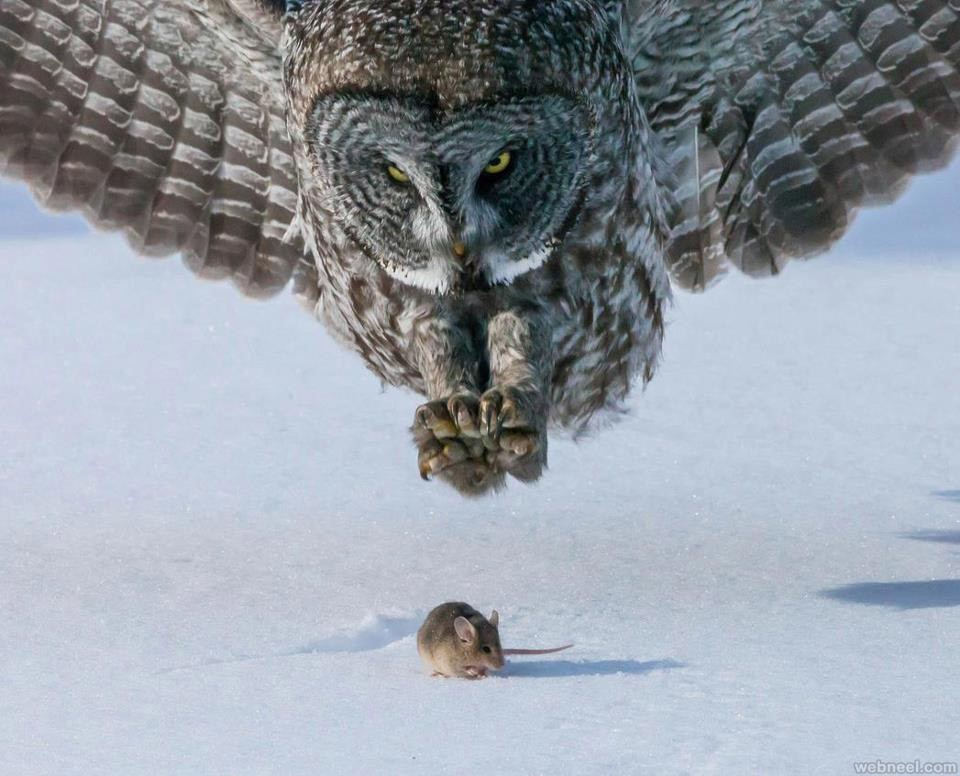
\includegraphics[scale=0.5]{Images/prepre.jpg}
\end{figure}

\end{titlepage}

\newlength{\realparindent}
\newlength{\realparskip}
\setlength{\realparindent}{\parindent}
\setlength{\realparskip}{\parskip}



\begin{nopagebreak}
{
\begin{center}
    \samepage
    \begin{tabular*}{\textwidth}{@{} l @{\extracolsep{\fill}}r@{}}
        \parbox[b]{11cm}{
            {\LARGE Aalborg Universitet} \\
            {\large Det Teknisk-Naturvidenskabelige Fakultet}\\
            {\large Instituttet For Matematiske Fag}
        }
        & 
\includegraphics[width=4cm]{aau_logo} \\
        \hline
    \end{tabular*}
    \vspace{0.4cm}

    \begin{tabular*}{\textwidth}{@{}l@{\extracolsep{\fill}}r@{}}
        \multicolumn{2}{@{}l@{}}{
            \begin{minipage}[t]{1.0\textwidth}
                \begin{description}
                    \item[Titel:]~\\
                    Rovdyr-byttedyr
                    \vspace{0.5cm}
                \end{description}
            \end{minipage}
        }\\
        \begin{minipage}[t]{0.49\textwidth}
            \begin{description}
                \item[Tema:]~\\
                Sædvanlige differentialligninger
                \vspace{0.5cm}
                \item[Projektperiode:]~\\
                P3, 2. september - 21. december 2016
                \vspace{0.5cm}

                \item[Projektgruppe:]~\\
                Gruppe G4-107
                \vspace{0.5cm}  
                \item[Gruppemedlemmer:]~\\
                Amalie Rhode Høgh Nielsen 

                Bue Juul Poulsgaard
                
                Emil Egekvist
                
                Mikkel Højlund Larsen
                
                Nicklas Søndergaard Pedersen
                
                Terkel Haar Jakobsen
                
                Thomas Dam Petersen
             
                \vspace{0.5cm}
                \item[Vejledere:]~\\
                Jon Johnsen
                \vspace{0.5cm}
                
                \item[Sideantal:]
                ?
                \item[Bilagsantal:]
                ?
                \item[Afsluttet den:]
                19/12-2016
            \end{description}
        \end{minipage}
        &
        \fbox{
            \begin{minipage}[t]{0.45\textwidth}
                \textbf{Synopsis:}\\
                % Der skal være normale afsnits-indryk,
                % selv om teksten står i en minipage:
                \setlength{\parindent}{\realparindent}
                \setlength{\parskip}{\realparskip}
                {\small 
                    bla bla
                }
            \end{minipage}
        }
        \\
    \end{tabular*}
\end{center}
}

\tiny{Rapportens indhold er frit tilgængeligt, men offentliggørelse (med kildeangivelse) må kun ske efter aftale med forfatterne.}
\end{nopagebreak}
\newpage
\tableofcontents
\newpage
\chapter*{Forord}
Tekst\\
\hfill \break

\makebox[2.5in]{\hrulefill} \hspace {1.0in}\makebox[2.5in]{\hrulefill} \\
Amalie Rhode Høgh Nielsen \makebox[3.1in][r]{Bue Juul Poulsgaard} \\

\vspace{.2in}
\makebox[2.5in]{\hrulefill} \hspace {1.0in}\makebox[2.5in]{\hrulefill} \\
Emil Egekvist \makebox[4.1in][r]{Mikkel Højlund Larsen} \\

\vspace{.2in}
\makebox[2.5in]{\hrulefill} \hspace {1.0in}\makebox[2.5in]{\hrulefill} \\
Nicklas Søndergaard Pedersen \makebox[3.05in][r]{Terkel Haar Jakobsen} \\

\vspace{.2in}
\makebox[2.5in]{\hrulefill}  \\
Thomas Dam Petersen \\
\chapter{Indledning}

%I dette projekt vil differentialligningssystemer blive bearbejdet, hvor der tages udgangspunkt i en case, hvor disse anvendes. Den udvalgte case for projektet omhandler Lotka-Volterra's rovdyr-byttedyr model.

%Rovdyr-byttedyr modellen er med til at beskrive en udvikling i et isoleret system, hvor man antager, at der ikke forekommer nogle ukendte variable. Der antages altså, at systemet er en akkurat afbildning af sammenhængen mellem rovdyr og byttedyr populationen under optimale forhold. Lotka-Volterra modellen er derfor et system, der kan udvides med flere variable for at gøre systemet mere virkelighedsnært. For eksempel kan man se på det udvidede system, der tager forbehold for, flere forskellige rovdyr, der konkurrerer om det samme byttedyr, eller en begrænset fødemængde til byttedyrene. I dette projekt vil der tages udgangspunkt i sidstnævnte variation af Lotka-Volterra's model, hvor modelleringsproblemet drastisk ændrer form til at være en differentialligningssystem, der inderholder logistisk vækst som en hovedingrediens (hvilken rolle den spiller kan uddybes senere).

%\textbf{Ovenstående er et alternativt forslag til midlertidig indledning :P (Systemet skal indsættes deroppe et sted)}


Dette projekt omhandler hvordan differentialligninger benyttes til modellering af fysiske og biologiske systemer. Intuitivt kunne man forestille sig, at i et isoleret system vil populationerne af rovdyr og byttedyr påvirke hinanden således, at hvis antallet af rovdyr stiger, vil antallet af byttedyr falde. Hvis antallet af byttedyr falder, vil rovdyrene ikke have nok at spise og dermed vil populationen af disse falde. Når populationen af rovdyr er tilstrækkeligt lav, vil antallet af byttedyr stige igen. 
Dette system kan modelleres matematisk ved brug af differentialligninger. Dette gjorde Vito Volterra og Alfred J. Lotka uafhængigt af hinanden i starten af 1900-tallet \citep{wikiLV}. De udarbejdede følgende model, som senere blev kendt som Lotka-Volterra-modellen:

\begin{equation}\label{byttedyr}
    \dfrac{db}{dt}(t) = (A-Br(t)) b(t), 
\end{equation}

\begin{equation}\label{rovdyr}
    \dfrac{dr}{dt}(t) = (Cb(t)-D) r(t),
\end{equation}

\hfill \break
hvor $A$, $B$, $C$ og $D$ betegner positive konstanter. Den første ligning beskriver, hvordan byttedyrspopulationen udvikler sig over tid, og den anden beskriver, hvordan rovdyrspopulationen udvikler sig over tid.\\ \hfill \break
Funktionen $b(t)$ er et udtryk for hvor mange byttedyr, der er til tiden $t$. Ligeledes er $r(t)$ et udtryk for hvor mange rovdyr, der er til tiden $t$. Det ses, at konstanten $A$ ganges på $b(t)$ i ligning \eqref{byttedyr}. Det vil sige at $A$ er et udtryk for hvor hurtigt byttedyrsbestanden vil stige uafhængigt af rovdyrsbestanden. Med andre ord, er det et udtryk for, i hvilken grad byttedyrene reproducerer. Konstanten $B$ ganges med $b(t)$ og $r(t)$, og er et udtryk for, i hvilken grad byttedyr bliver ædt af rovdyr. Der bliver således ædt flest byttedyr, hvis der både er mange rovdyr og mange byttedyr, hvilket intuitivt giver god mening. Betragtes hele ligning \eqref{byttedyr}, ses det, at ændringen i antallet af byttedyr er lig med antallet af nye byttedyr, $Ab(t)$, minus antallet af byttedyr, som bliver ædt, $Br(t)b(t)$.\\ \hfill \break
I ligning \eqref{rovdyr} ses det, at leddet som beskriver tilvæksten i rovdyr er $Cb(t)r(t)$. Dermed er $C$ et udtryk for, i hvilken grad rovdyrene reproducerer. I modellen antages det altså, at rovdyrenes reproduktion er proportional med antallet af byttedyr. Konstanten $D$ ganges på $r(t)$ og er et udtryk for hvor mange rovdyr der dør. Antallet af rovdyr, der dør, er således højere jo flere rovdyr, der er. \\ \hfill \break
I modellen er der taget en række antagelser om systemet, for at kunne modellere det. Disse antagelser er \citep{wikiLV}:
\begin{enumerate}
    \item Byttedyrene finder altid rigeligt føde.
    \item Rovdyrenes forsyning af føde afhænger udelukkende af størrelsen af bytterdyrspopulationen.
    \item Hastigheden hvormed en populations størrelse ændrer sig er proportional med populationens størrelse.
    \item Miljøet ændrer sig ikke til fordel for en af populationerne, og genetisk tilpasning har ingen konsekvenser.
    \item Rovdyr har uendelig appetit.
\end{enumerate}
I dette projekt beskæftiger vi os ikke med punkterne 2-5, men vi vil undersøge, hvilken indflydelse det har på systemet, hvis mængden af føde til byttedyrene er begrænset. Derudover vil vi beskrive systemet i ligninger \eqref{byttedyr} og \eqref{rovdyr} i lyset af teorien om differentialligninger.
\hfill \break
\section{Problemformulering} 
Hvordan bruges et system af differentialligninger til at modellere et byttedyr-rovdyr system, og hvilken indflydelse har det på systemet, hvis mængden af føde til byttedyrene er begrænset?
%Hvordan vil en begrænset mængde føde til byttedyrene influere systemets stabilitet?



\newpage
\chapter{Differentialligninger}
I det følgende kapitel vil teorien for differentialligninger og løsninger dertil blive gennemgået, da en forståelse af denne er nødvendig for at kunne udvide Lotka-Volterra's model og vurdere denne. 

\section{Sædvanlige differentialligninger}
Først defineres en sædvanlig differentialligning, hvori $I$ er et interval i $\mathbb{R}$:
\begin{definition}[Sædvanlig differentialligning (ODE)]
En sædvanlig differentialligning er en ligning på formen: \hfill \break
$$G(t,y(t),y'(t), \hdots , y^{(n)}(t))=0,$$
hvor:
\begin{itemize}
    \item $t \in I \subseteq \mathbb{R}$ er en uafhængig variabel.
    \item $y(t) = y, \ y \in \mathbb{R}$ er en afhængig variabel.
    \item $G:A \to \mathbb{R}$ er en funktion, hvor $A \subseteq \mathbb{R}^{n+2}$ er en åben delmængde af $\mathbb{R}^{n+2}$.
\end{itemize}.
\end{definition}

Ordenen, $n$, af en ODE angiver, at den $n$'te afledte af den afhængige variabel $y(t)$ er den højest afledte. 
Sædvanlige differentialligninger kan løses ved at bestemme en løsning til disse:

\begin{definition} [Løsning til ODE]
En løsning til en ODE af $n$'te orden, er en funktion, $\phi: I\to \mathbb{R}$ som opfylder
\begin{itemize}
    \item $\phi(t)$ er $n$ gange differentiabel
    \item $\forall t\in I: (t,\phi(t),\phi'(t),\hdots,\phi^n(t))\in A$
    \item $\forall t\in I: G(\phi(t),\phi'(t),\hdots,\phi^n(t))=0$
\end{itemize}

En partikulær løsning er en bestemt løsning, mens den fuldstændige løsning er familien af alle løsninger til ODE.
\end{definition}

Ved en ODE er det væsentligt at skelne mellem lineære og ikke-lineære sædvanlige differentialligninger, da disse har forskellige løsningsmetoder og beskriver forskellige situationer.

\begin{definition}[Sædvanlig lineær differentialligning (OLDE)]\label{OLDE}En ODE af $n$'te orden kaldes lineær, hvis de afledte op til orden $n$ indgår i form af en linearkombination. Altså: \\ 
$$a_{n}(t)y^{(n)}  + a_{n-1}(t)y^{(n-1)}+ \hdots + a_{1}(t)y' + a_{0}(t)y = f(t)$$
Da $a_n(t)\neq 0$, fås der ved normering:

$$y^{(n)}+P_{n-1}(t)y^{(n-1)}+\hdots +P_0(t)y=Q(t)$$ 

Her er: $P_0(t)=\frac{a_0(t)}{a_n(t)} , P_1(t)=\frac{a_1(t)}{a_n(t)}, \hdots, P_{n-1}(t)=\frac{a_{n-1}(t)}{a_n(t)}$ og $Q(t)=\frac{f(t)}{a_n(t)}$
\end{definition}

For en OLDE defineres følgende: 
\begin{definition}[Homogenitet]
En ODE kaldes homogen, hvis den kan skrives på formen: 
$$y^{(n)}(t)=G(y,y', \hdots, y^{(n-1)})$$ 
Altså hvis den n'te afledede $y^{(n)}$ kan skrives på en form, hvor en eksplicit funktion af udelukkende den uafhængige variabel $t$ ikke indgår. En inhomogen ODE er på formen: 
$$y^{(n)}(t)=G(y,y',\hdots, y^{(n-1)})+f(t)$$
I dette tilfælde kaldes $f(t)$ en inhomogenitet. ODE der indeholder en inhomogenitet kaldes inhomogene, mens ODE, der ikke indeholder en inhomogenitet, kaldes homogen.
\end{definition}
Til den inhomogene OLDE, $G(y,y',...,y^{(n)})=f(t)$, kalder vi ligningen, $G(t,y,y',...,y^{(n)})=0$, den associerede homogene ODE. 

%\begin{mytheo}{Generel løsning for homogene OLDE}{}
%    Lad $y_1,y_2,\hdots,y_n$ være $n$ lineære uafhængige løsninger til den homogene ligning:
%    \begin{equation}\label{glhomo}
%        a_n(t)y^{(n)}+\hdots +a_1(t)y'+a_0(t)y=0
%    \end{equation}
%    på et åbent interval $I$, hvor $p_i$ er sammenhængende.
%    Hvis $Y$ er en hvilken som helst løsning til \eqref{glhomo}, da vil der eksistere $c_1,c_2,\hdots %c_n$ således at:
%    $$Y(t)=c_1y_1(t)+c_2y_2(t)+\hdots+c_ny_n(t)$$
%    for alle $x\in I$
%\end{mytheo}
%Dermed er alle løsninger til en homogen $n$'te orden OLDE en lineær kombination, 
%$$y=c_1y_1+c_2y_2+\hdots+c_ny_n$$,
%af enhver $n$ given lineær uafhængig løsning. Baseret på dette kalder vi en sådan lineær kombination %en generel løsning for en homogen OLDE.

\begin{mytheo}{Den fuldstændige løsning til en inhomogen OLDE}{}
Betragt en inhomogen OLDE på formen: 
\begin{equation}\label{linhomo}
a_n(t)y^{(n)}+\hdots +a_1(t)y'+a_0(t)y=F(t), \enspace t\in I
\end{equation}
med den associerede homogene OLDE:
\begin{equation}\label{lhomo}
a_n(t)y^{(n)}+\hdots +a_1(t)y'+a_0(t)y=0, \enspace t\in I
\end{equation}
har den fuldstændige løsning:
$$y(t)=y_p+y_f$$
Hvor $y_p$ er en partikulær løsning til ligningen og $y_f$ er en vilkårlig løsning til den associerede homogene OLDE.       
\end{mytheo}

\begin{proof}\hfill \break
Antag at en partikulær løsning $y_p$ til $\eqref{linhomo}$ er kendt og at $Y$ er en vilkårlig anden løsning til $\eqref{linhomo}$. Hvis $y_f=Y-y_p$, så får vi ved at indsætte $y_f$ i differentialligningen:
\begin{align*}
    a_n(t)y_f^{(n)}+\hdots +a_1(t)y_f'+a_0(t)y_f&=
    (a_n(t)Y^{(n)}+\hdots +a_1(t)Y'+a_0(t)Y)\\
    &-(a_n(t)y_p^{(n)}+\hdots +a_1(t)y_p'+a_0(t)y_p)\\
    &=F(t)-F(t)=0
\end{align*}
Dermed er $y_f=Y-y_p$ en løsning til den associerede homogene ligning \eqref{lhomo}. Den kan omskrives til
$$Y=y_f+y_p$$
\textbf{ANDEN VEJ OGSÅ!}
Dermed er det bevist at en generel løsning til \eqref{linhomo} er summen af en vilkårlige løsning $y_f$ og den partikulære løsning $y_p$ til \eqref{lhomo}.
\end{proof}

\section{Førsteordens differentialligninger}
I afsnittet forinden blev det kort introduceret, hvad en differentialligning er, de afhængige og uafhængige variabler den er opbygget af, de konstanter der indgår deri, samt formen af løsninger dertil. I det følgende vil vi se isoleret på første ordens differentialligninger samt løsningsmetoder dertil, da disse er byggesten til Lotka-Volterra's model.
Følgende afsnit er baseret på \citep{JAB}, hvis andet ikke er noteret.
\subsection{Separable differentialligninger}
Følgende beskriver en central metode til omskrivning af differentialligninger og er dermed anvendelig, når en løsning søges.
\begin{definition}[Separabel differentialligning]
En førsteordens ODE kaldes separabel, hvis den kan skrives på formen, $$y'(t)=g(t)p(y(t))$$ hvor $g(t)$ kun afhænger af $t$, og $p(y(t))$ kun afhænger af $y(t)$.
\end{definition}

\begin{mytheo}{Løsning til separable differentialligninger}{LSD}
Lad en funktion $p$ være kontinuert og $p(y(t)) \neq 0 \ \forall y$. Da vil løsningen til en førsteordens separabel ODE:
$$y'(t)=g(t)p(y(t))$$
også være en løsning til ligningen: 
$$\int \frac{1}{p(y(t))}dy=\int g(t)dt$$
\end{mytheo}

\begin{proof}\hfill \break
Vi starter med $$y'(t)=g(t)p(y(t))\Longleftrightarrow \frac{dy}{dt} = g(t)p(y(t))$$
Hvis funktionen $p$ er kontinuert, og $p(y)\neq 0 \forall y$, kan man omskrive formlen på følgende måde:
\begin{align*}
    \frac{dy}{dt} &= g(t)p(y)\\
    \frac{1}{p(y)}\frac{dy}{dt} &= g(t)
\end{align*}
Hvis $H(y)$ er en funktion, således at $H'(y)=\frac{1}{p(y)}$, så har vi: $$H'(y) \frac{dy}{dt}=g(t)$$
Ved at anvende reglen for differentiation af en sammensat funktion, som siger $(f(g(x)))'=f'(g(x))g'(x)$, får vi:
$$(H(y(t)))'=g(t)$$
og ved at integrere på begge sider i forhold til $t$ får vi:
$$H(y)=\int g(t) dt$$
Her må det gælde at $H(y)=\int \frac{1}{p(y)}dy$, hvilket resulterer i: $$\int \frac{1}{p(y)}dy=\int g(t) dt$$
\end{proof}

\begin{Example}\hfill \break
\textnormal{Betragt følgende funktion} $$\frac{dy}{dt}=\frac{t^2+3}{y}$$ \textnormal{Ovenstående ligning er separabel, og vi kan derfor separere og omskrive til følgende:} $$(y)dy=(t^2+3)dt$$ \textnormal{Derefter integreres der på begge sider:} $$\int (y)dy=\int (t^2+3)dt\Leftrightarrow$$ $$\frac{y^2}{2}=\frac{t^3}{3}+3t+C$$ \textnormal{Til sidst løses ovenstående ligning i forhold til} $y$:$$y=\sqrt{\frac{2t^3}{3}+6t+2C}$$ \textnormal{Eftersom $C$ er en konstant af enhver størrelse, så er $2C$ dermed også en konstant af enhver størrelse. Derfor kan $2C$ i ligningen erstattes med en konstant $K$, hvilket resultere i:} $$y=\sqrt{\frac{2t^3}{3}+6t+K}$$
\end{Example}

\subsection{Lineære differentialligninger}
Følgende er med til at skabe en forståelse for løsninger til lineære differentialligninger og afdækkes, da de første systemer af differentialligninger, der introduceres i projektet, er lineære.
\hfill \break

En førsteordens OLDE er en ligning på formen: \\ 
$$a_{1}(t) \frac{dy}{dt} + a_{0}(t)y = f(t)$$ Hvor $t$ er den uafhængige variabel. \hfill \break

Vi betragter nu to tilfælde for koefficienten $a_0$, hvor $a_0(t) = 0$ og $a_0(t) = a_1'(t)$. Hvis $a_0(t) = 0$ reduceres ligningen til $a_1(t)\frac{dy}{dt} = f(t)$.  
\begin{Example}\hfill \break
\textnormal{Antag at vi har en førsteordens OLDE, som følger, hvor $a_0(t) = 0$.}\\
\hfill \break
\centerline{$0y - 6t = -(3t^2) \frac{dy}{dt}$ $\Rightarrow$ $3t^2 \frac{dy}{dt} = 6t$}
\hfill \break
\centerline{$y'(t) = \frac{6t}{3t^2}$ $\Rightarrow$ $y(t) = \int \frac{6t}{3t^2}dt$}
\hfill \break
\textnormal{Løsningen kan derfor findes ved simpel isolering af variabler og integration.}
\end{Example}

For det andet tilfælde får vi af produktreglen at $$a_1(t)y'(t) + a_0(t)y(t) = a_1(t)y'(t) + a_1'(t)y(t) = \frac{d}{dt}(a_1(t)y(t))$$Da har vi $$\frac{d}{dt}(a_1(t)y(t)) = f(t)$$ hvoraf løsningen let kan findes.

\begin{Example} \hfill \break
\textnormal{Antag at vi har en førsteordens OLDE, som følger, hvor $a_0(t) = a_1'(t)$} \\
\hfill \break
$$t^2 = \frac{1}{t}y'(t) -\frac{1}{t^2}y(t) = \frac{d}{dt}(\frac{1}{t}y(t))\Leftrightarrow$$
$$\frac{d}{dt}(\frac{1}{t}y(t)) = t^2\Leftrightarrow$$
$$\frac{1}{t}y(t) = \int t^2dt \Leftrightarrow$$ $$ y(t) = t \int t^2dt$$
\hfill \break
\textnormal{Dermed kan vi igen isolere og integrere for at finde løsningen.}
\end{Example}

Der eksisterer mange tilfælde, hvor OLDE ikke umiddelbart kan reduceres til en af de to ovenstående former, hvorfor det ses nødvendigt at finde en anden metode til løsning af disse. Derfor omskriver vi OLDE, som vist i definition \ref{OLDE}: $${y'(t) + \frac{a_0(t)}{a_1(t)}y(t) = \frac{b(t)}{a_1(t)}} \Leftrightarrow$$
$$y'(t) + P(t)y(t) = Q(t)$$ hvor $y'(t) + P(t)y(t) = Q(t)$ er den normerede ligning. Derudover vil vi anvende en integrationsfaktor.

\begin{definition}[Integrationsfaktor]\label{IntFak}
En funktion $\mu (t)$, der ved multiplikation ændrer en lineær normeret differentialligning til en ligning på formen: $$\frac{d}{dt}(\mu (t)y(t)) = \mu (t)Q(t)$$ kaldes en integrationsfaktor.  
\end{definition}

Denne integrationsfaktor kan benyttes til at finde en generel løsning til en OLDE, og det er illustreret ved nedenstående sætning.

\begin{mytheo}{Løsning til OLDE}{}
For enhver OLDE, der kan skrives på formen:
\begin{equation}\label{LOLDE}
\frac{dy}{dt}+P(t)y=Q(t)
\end{equation}
eksisterer der en integrationsfaktor $\mu(t)$, hvorom der gælder, at: $$y(t)=\frac{1}{\mu (t)}(\int \mu (t)Q(t)dt+K)$$ er den generelle løsning til OLDE.
\end{mytheo}

\begin{proof}
Vi anvender en integrationsfaktor $\mu(t)$ ved at gange denne til den normerede ligning.
\begin{equation}\label{Intfaktor}
\mu (t)y'(t) + \mu (t)P(t)y(t) = \mu (t)Q(t) 
\end{equation}
Per definition \ref{IntFak} må $\mu ' = \mu P$ og da kan vi udlede af \ref{th:LSD} at $\frac{1}{\mu}d\mu = P(t)dt$.
Ligning \eqref{Intfaktor} omskrives til $$\frac{d}{dt}(\mu (t)y(t)) = \mu (t)Q(t)$$ 
med $\mu (t)$ som den ovenstående, kan vi finde en generel løsning til (\ref{LOLDE}) ved integration på begge sider og derefter isolere $y(t)$:
\begin{equation}
y(t)=\frac{1}{\mu (t)}(\int \mu (t)Q(t)dt+K)
\end{equation}
\end{proof}

\begin{Example}
\textnormal{Antag at vi har en førsteordens OLDE:}
$$2ty'(t) + 4y(t) = 6t^2$$
\textnormal{Hvis vi dividerer igennem med 2t fås:}
$$y'(t) + \frac{2}{t}y(t) = 3t$$
$$\int P(t)dt = \int \frac{2}{t}dt = 2ln(t)$$
\textnormal{Da har vi integrationsfaktoren,} $\mu = e^{2ln|t|} = e^{ln(t^2)} = t^2$. \textnormal{Nu ganges $\mu$ på den normerede ligning:}
$$t^2 \frac{dy}{dt} + 2ty = 3t^3\Leftrightarrow$$
$$\frac{d}{dt}(t^2y) = 3t^3 \Leftrightarrow  t^2y = \int 3t^3dt = \frac{3}{4}t^4 + K$$
\textnormal{Da får vi:} 
$$y = \frac{3}{4}t^4t^{-2} + Kt^{-2} = \frac{3}{4}t^2 + K \frac{1}{t^2}$$
\end{Example}

%%\begin{Example}
%%Antag at vi har en førsteordens OLDE:\\
%%\hfill \break
%%\centerline{$ty'(t) + 2y(t) = t^2 - t + 1$}
%%\hfill \break
%%Hvis vi dividerer igennem med 2t fås:\\
%%\hfill \break
%%\centerline{$y'(t) + \frac{2}{t}y(t) = t + -1 \frac{1}{t}$}
%%\hfill \break
%%\centerline{$\int P(t)dt = \int \frac{2}{t}dt = e^2ln(t)}
%%\hfill \break
%%Da har vi integrationsfaktoren, $\mu = e^{2ln|t|} = e^{ln(t^2)} = t^2$\\
%%\hfill \break
%%\centerline{$t^2 \frac{dy}{dt} + 2ty = \frac{3t}{2}$}
%%\hfill \break
%%\centerline{$\frac{d}{dt}(t^2y) = \frac{3t}{2}$ $\rightarrow$ $t^2y = \int \frac{3t}{2}dt = \frac{3}{4}t^2 + K$}
%%\hfill \break
%%Da får vi: \\
%%\hfill \break
%%\centerline{$y = \frac{3}{4}t^2t^{-2} = \frac{3}{4} + Kt^{-2}$}
%%\end{Example}
%% kilde: http://tutorial.math.lamar.edu/Classes/DE/Linear.aspx

\section{Begyndelsesværdiproblemer}
Begyndelsesværdiproblemer omfatter både enkeltstående differentialligninger og systemer af differentialligninger, hvorfor det vil blive beskrevet i det følgende.
\begin{definition}[Begyndelsesværdiproblem (IVP)]
Et begyndelsesværdiproblem (IVP) er en ODE med en betingelse, som $y, y',\hdots, y^{(n)}$ skal overholde for en specifik værdi af den uafhængige variabel, altså:
\begin{align*}
    y(t_0) &= y_0 \\
    y'(t_0) &= y_1 \\
    &\vdots \\
    y^{(n)}(t_0) &= y_n
\end{align*}
\end{definition}

\begin{Example}\textbf{IVP}\hfill \break
\textnormal{Betragt følgende IVP:}\hfill \break
\centerline{$y+y''=0, t \in I \subseteq \mathbb{R}$}
\centerline{bbt:}
\centerline{$y(0)=1$}
\centerline{$y'(0)=0$} \hfill \break
\textnormal{Det ses hurtigt, at $y(t)=\cos(t)$ er en løsning til dette IVP. Dette kan efterprøves:}
\begin{align*}
    y+y''&=0 \\
    \cos(t)+(-\cos(t))&=0 \\
    y(0)=\cos(0)&=1\\
    y'(0)=-\sin(0)&=0\\ 
\end{align*}
\textnormal{Dermed er dette IVP løst.}
\end{Example}

\begin{mytheo}{Eksistens- og entydighedssætningen}
GGivet et førsteordens IVP, $y'(t)=f(t,y)$, hvor 

\begin{enumerate}
    \item $y(t_0)=y_0$
    \item $f:(a,b) \times (c,d) \rightarrow \mathbb{R}$
    \item $\frac{\partial}{\partial y}f$ er kontinuert
    \item $(t_0,y_0) \in (a,b) \times (c,d)$
\end{enumerate}

da findes en entydig løsning $\phi(t)$ defineret på $(\alpha,\beta)\subseteq (a,b)$, hvor $t_0 \in (\alpha, \beta)$ 
\end{mytheo}

Til at bevise denne sætning kan man benytte Lipschitz betingelser samt Banachs fix-punkt sætning, men disse vil ikke blive beskrevet yderligere i denne rapport, da fokus, for projektet, ligger på at undersøge en udvidelse af Lotka-Volterra's model. Samtidigt er beviset og alle forudsætninger dertil tidskrævende og omhandler ikke direkte problemstillingen. 

\section{Andenordens differentialligninger}
Følgende afsnit inkluderes som følge af studieordningen, som sætter projektets rammer, men ligeledes fordi, man kan omskrive andenordens ODEs til koblede systemer af differentialligninger.
\subsection{Homogene lineære andenordens ODE med konstante koefficienter}
Det følgende er baseret på \citep[s. 221]{JAB}. \\ \hfill \break En homogen lineær andenordens ODE med konstante koefficienter er en ODE på formen: \hfill \break
\begin{equation}
\label{homlinandord}
    a_2y''(t)+a_1y'(t)+a_0y(t)=0
\end{equation} \hfill \break
Hvor $a_2,a_1,a_0\in \mathbb{C}$ er de konstante koefficienter, og $a_2\neq 0$. \hfill \break

\begin{definition}[Den karakteristiske ligning]
Ligningen 
$$a_2r^2+a_1r+a_0=0$$
hvor $a_2, a_1$ og $a_0$ er koefficienterne fra (\ref{homlinandord}), kaldes den karakteristiske ligning for (\ref{homlinandord}).
\end{definition} 
\hfill \break
Det bemærkes at for en inhomogen andenordens ODE på formen
$$a_2r^2+a_1r+a_0=f(t)$$
kaldes ligningen i ovenstående definition også for den tilhørende karakteristiske ligning.
Den  karakteristiske ligning er et andengradspolynomium, og de værdier af $r$, som opfylder denne ligning, er vigtige, som det fremgår af følgende proposition: \hfill \break
\begin{prop}{Løsning af homogen andenordens (ODE)}{losprop2ordhom}\label{losprop2ordhom}
Funktionen $y(t)=e^{rt}$ er en løsning til (\ref{homlinandord}), hvis og kun hvis $r$ er en løsning til den karakteristiske ligning for (\ref{homlinandord}).
\end{prop}
\hfill \break
\begin{proof} \hfill \break
Vi sætter $y=e^{rt}$ og bemærker, at $y'=re^{rt}$ samt $y''=r^2e^{rt}$. Nu skrives (\ref{homlinandord}): \hfill \break
 $$a_2r^2e^{rt}+a_1re^{rt}+a_0e^{rt}=0 \Leftrightarrow$$ 
 $$e^{rt}(a_2r^2+a_1r+a_0)=0$$
 Da $e^{rt}>0$ må det ifølge nulreglen gælde at: \hfill \break
 $$a_2r^2+a_1r+a_0=0$$
\end{proof} \\ 
\hfill \break

Vi har altså en simpel metode til at finde en partikulær løsning til (\ref{homlinandord}):\hfill \break

\begin{Example}\label{ekspartlos} \textbf{Partikulær løsning}\hfill \break
\textnormal{Betragt følgende ODE:}\\ \hfill \break
\centerline{$-y''(t)+2y'(t)+3y(t)=0$}\\ \hfill \break
\textnormal{Nu kan vi finde en partikulær løsning ved først at finde rødderne til den karakteristiske ligning:}\\ \hfill \break
\centerline{$-r^2+2r+3=0$}\\ \hfill \break
\textnormal{Rødderne er i dette tilfælde:}\\ \hfill \break
\centerline{$r_1=\frac{-2+\sqrt{2^2-4\cdot (-1)\cdot 3}}{2\cdot (-1)}=-1$ \textnormal{og} $r_2=\frac{-2-\sqrt{2^2-4\cdot (-1)\cdot 3}}{2\cdot (-1)}=3$} \\ \hfill \break
\textnormal{Vælger vi for eksempel $r_2$ og sætter $y(t)=e^{3t}$, kan vi tjekke, at det er en partikulær løsning til ovenstående ODE:}\\ \hfill \break
\centerline{$(-1)\cdot3^2e^{3t}+2\cdot 3e^{3t}+3e^{3t}=0e^{3t}=0$}\\ \hfill \break
\textnormal{På samme måde kan det vises at $e^{(-1)t}$ også er en partikulær løsning.}
\end{Example}\hfill \break

I det følgende, som er baseret på \citep{2ordhom}, ønsker vi en metode til at finde den fuldstændige løsning til (\ref{homlinandord}). Først skal vi vise to propositioner:\hfill \break
\begin{prop}{Linearkombination af løsninger}
HHvis $y_1(t)$ og $y_2(t)$ begge er løsninger til ligning (\ref{homlinandord}), og $k_1,k_2\in \mathbb{C}$ er arbitrære konstanter, så er \hfill \break
$$y(t)=k_1y_1(t)+k_2y_2(t),$$ \hfill \break
også en løsning til ligning (\ref{homlinandord}).
\end{prop}
\hfill \break
\begin{proof}\hfill \break
Lad $y_1$ og $y_2$ være løsninger til ligning (\ref{homlinandord}), og lad $k_1,k_2\in \mathbb{C}$ være givet. Nu tjekker vi om $k_1y_1(t)+k_2y_2(t)$ er en løsning til ligning (\ref{homlinandord}):
\hfill \break
\begin{align*}
a_2y''(t)+a_1y'(t)+a_0y(t)&=a_2(k_1y_1(t)+k_2y_2(t))''+a_1(k_1y_1(t)+k_2y_2(t))'+a_0(k_1y_1(t)+k_2y_2(t)) \\
&=a_2(k_1y_1''(t)+k_2y_2''(t))+a_1(k_1y_1'(t)+k_2y_2'(t))+a_0(k_1y_1(t)+k_2y_2(t)) \\
&=a_2k_1y_1''(t)+a_2k_2y_2''(t)+a_1k_1y_1'(t)+a_1k_2y_2'(t)+a_0k_1y_1(t)+a_0k_2y_2(t) \\
&=k_1(a_2y_1''(t)+a_1y_1'(t)+a_0y_1(t))+k_2(a_2y_2''(t)+a_1y_2'(t)+a_0y_2(t))
\end{align*}
\hfill \break
Da $y_1(t)$ er en løsning, ved vi at $a_2y_1''(t)+a_1y_1'(t)+a_0y_1(t)=0$, og da $y_2(t)$ er en løsning, ved vi at $a_2y_2''(t)+a_1y_2'(t)+a_0y_2(t)=0$. Altså har vi:\hfill \break
$$k_1(a_2y_1''(t)+a_1y_1'(t)+a_0y_1(t))+k_2(a_2y_2''(t)+a_1y_2'(t)+a_0y_2(t))=k_1\cdot 0+k_2\cdot 0=0$$\hfill \break
Dermed er $k_1y_1(t)+k_2y_2(t)$ en løsning til (\ref{homlinandord}).
\end{proof}\\
\hfill \break
\begin{mytheo}{Fuldstændig løsning}
JHvis $y_1(t)$ og $y_2(t)$ er lineært uafhængige løsninger til ligning (\ref{homlinandord}), og $k_1 \in \mathbb{C}$ og $k_2\in \mathbb{C}$ er arbitrære konstanter, så er den fuldstændige løsning til ligning (\ref{homlinandord}) givet ved: \hfill \break
$$y(t)=k_1y_1(t)+k_2y_2(t)$$
\end{mytheo}
\hfill \break
Vi har vist at $y(t)$ er en løsning, men vi mangler at vise, at enhver løsning kan skrives på den form. Beviset bygger på eksistens og entydighedssætningen. Beviset føres ikke i dette projekt, men bevises i (INDSÆT KILDE HER!(Jeg kan ikke finde nogen kilde, hvor det bevises..))\\
\hfill \break
Vi skal altså kende to lineært uafhængige partikulære løsninger for at kunne skrive den fuldstændige løsning op. Proposition \ref{losprop2ordhom} siger, at vi kan finde partikulære løsninger ved at løse den karakteristiske ligning. Som bekendt kan et andengradspolynomium enten have to forskellige reelle rødder, én reel rod eller to forskellige komplekse rødder. Vi viser for hvert tilfælde, hvordan den fuldstændige løsning findes. \\ \hfill \break
\textbf{Tilfælde 1}\hfill \break
Hvis den karakteristiske ligning har to forskellige reelle rødder, $r_1$ og $r_2$, så er løsningerne $e^{r_1t}$ og $e^{r_2t}$ lineært uafhængige. Det ses let, da der ikke findes nogen konstant, $k\in \mathbb{C}$, så $e^{r_1t}=ke^{r_2t}$ for alle $t$. Den fuldstændige løsning kan derfor skrives: \hfill \break
$$y(t)=k_1e^{r_1t}+k_2e^{r_2t}$$\hfill \break
Hvor $k_1,k_2\in \mathbb{C}$ er arbitrære konstanter.\\ \hfill \break
\begin{Example}\textbf{To reelle løsninger}\hfill \break
\textnormal{Betragt ligningen:} \hfill \break
\centerline{$-y''(t)+2y'(t)+3y(t)=0$}\\ \hfill \break
\textnormal{fra eksempel \ref{ekspartlos}. I eksemplet fandt vi løsningerne: $y_1(t)=e^{-t}$ og $y_2(t)=e^{3t}$. Den fuldstændige løsning kan således skrives:}\hfill \break
$$y(t)=k_1e^{-t}+k_2e^{3t}$$
\end{Example}
\hfill \break
\textbf{Tilfælde 2}\hfill \break
Hvis den karakteristiske løsning har én reel rod, $r$, så er diskriminanten som bekendt 0. Derfor har vi fra den karakteristiske ligning: \hfill \break
$$r=\frac{-a_1}{2a_2}\Leftrightarrow 2a_2r+a_1=0$$
\hfill \break
Det skal vi bruge til at vise, at udover $e^{rt}$, så er $y(t)=te^{rt}$ også en partikulær løsning til ligning (\ref{homlinandord}). Bemærk først at $y'(t)=e^{rt}+tre^{rt}$ og $y''(t)=2re^{rt}+tr^2e^{rt}$. Det sætter vi nu ind i ligning (\ref{homlinandord}): 
\hfill \break
\begin{align*}
a_2(2re^{rt}+tr^2e^{rt})+a_1(e^{rt}+tre^{rt})+a_0te^{rt}&=\\
e^{rt}(2a_2r+a_1)+te^{rt}(a_2r^2+a_1r+a_0)&=e^{rt}\cdot 0+te^{rt}\cdot 0=0
\end{align*}
\hfill \break
Så $te^{rt}$ er altså en løsning. det er nemt at se at $e^{rt}$ og $te^{rt}$ er lineært uafhængige, og vi kan dermed skrive den fuldstændige løsning op:\hfill \break
$$y(t)=k_1e^{rt}+k_2te^{rt}$$ \hfill \break
\begin{Example}\textbf{Én reel løsning}\hfill \break
\textnormal{Lad følgende ODE være givet:}\hfill \break
$$y''(t)+2y'(t)+y(t)=0$$\hfill \break
\textnormal{Den karakteristiske ligning $r^2+2r+1=0$ har kun én løsning, da deskriminanten $d=2^2-4\cdot 1\cdot 1=0$. Løsningen er $r=\frac{-2}{2\cdot 1}=-1$.}\\ \hfill \break
\textnormal{Dermed kan den fuldstændige løsning til ovenstående ODE skrives:}\hfill \break
$$y(t)=k_1e^{-t}+k_2te^{-t}$$
\end{Example}
\hfill \break
\textbf{Tilfælde 3}\hfill \break
Hvis den karakteristiske ligning har to komplekse rødder, $r_1$ og $r_2$, er diskriminanten negativ, og de to rødder er $r_1=\frac{-a_1}{2a_2}+i\frac{-a_1^2+4a_2a_0}{2a_2}$ og $r_2=\frac{-a_1}{2a_2}-i\frac{-a_1^2+4a_2a_0}{2a_2}$. For nemheds skyld betegner vi dog rødderne på følgende måde: $r_1=\alpha+i\beta$ og $r_2=\alpha-i\beta$. Ifølge proposition \ref{losprop2ordhom} er $e^{r_1t}$ og $e^{r_2t}$ løsninger til ligning (\ref{homlinandord}), og det er dermed nok at vise, at de to løsninger er lineært uafhængige. Det er let at indse, da $\beta \neq 0$. Hvis $c_1\in \mathbb{C}$ og $c_2 \in \mathbb{C}$ er arbitrære konstanter kan den fuldstændige løsning dermed skrives:\hfill \break
$$y(t)=c_1e^{(\alpha+i\beta)t}+c_2e^{(\alpha-i\beta)t}$$ \hfill \break
Vi vil imidlertid gerne finde en lettere måde at udtrykke den fuldstændige løsning på. Vi bruger Eulers formel\citep[s. 27]{JAB}, $e^{i\beta}=\cos(\beta)+i\sin(\beta) \enspace \forall \beta \in \mathbb{R}$, og regnereglen, $e^{\alpha+i\beta}=e^{\alpha}e^{i\beta}$, og skriver den fuldstændige løsning:\hfill \break
\begin{align}
y(t)&=c_1'e^{(\alpha+i\beta)t}+c_2'e^{(\alpha-i\beta)t} \notag \\
&=c_1'e^{\alpha t}(\cos(\beta t)+i\sin(\beta t))+c_2'e^{\alpha t}(\cos(\beta t)-i\sin(\beta t)) \notag \\
&={\alpha t}(c_1'\cos(\beta t)+c_1'i\sin(\beta t)+c_2'\cos(\beta t)-c_2'i\sin(\beta t)) \notag \\
&=e^{\alpha t}((c_1'+c_2')\cos(\beta t)+i(c_1'-c_2')\sin(\beta t)) \notag \\
&=e^{\alpha t}(c_1\cos(\beta t)+c_2\sin(\beta t)) 
\end{align}
hvor $c_1=c_1'+c_2'$ og $c_2=i(c_1'-c_2')$.\hfill \break
\begin{Example}\textbf{To komplekse rødder} \hfill \break
\textnormal{Betragt følgende (ODE):}\hfill \break
$$y''(t)+2y'(t)+2y(t)=0$$\hfill \break
\textnormal{Den karakteristiske ligning har følgende løsninger:} \hfill \break
$$r_1=\frac{-2+\sqrt{2^2-4\cdot 1\cdot 2}}{2\cdot 1}=\frac{-2+\sqrt{-4}}{2}=\frac{-2+2i}{2}=-1+i$$
$$r_2=\frac{-2-\sqrt{2^2-4\cdot 1\cdot 2}}{2\cdot 1}=\frac{-2-\sqrt{-4}}{2}=\frac{-2-2i}{2}=-1-i$$\hfill \break
\textnormal{Dermed kan den fuldstændige løsning skrives:}\hfill \break
$$y(t)=e^{-t}(c_1\cos(t)+c_2\sin(t))$$
\end{Example}

\subsection{Inhomogene lineære andenordens ODE med konstante koefficienter}\label{ila} 
For fuldstændighedens skyld opsummeres de ubestemte koefficienters metode. Dette afsnit er baseret på \citep[s. 240-246]{JAB}.\hfill \break
En inhomogen lineær andenordens ODE med konstante koefficienter skrives på formen:

\begin{equation}
\label{inhomlinandord}
    a_2y''(t)+a_1y'(t)+a_0y(t)=f(t)
\end{equation} \hfill \break
Hvor $a_2,a_1,a_0\in \mathbb{C}$ er de konstante koefficienter og $a_2 \neq 0$. I dette afsnit vil de ubestemte koefficienters metode, som er en fremgangsmåde, hvorpå inhomogene andenordens ODE's kan løses, blive gennemgået.
Metoden går i alt sin enkelthed ud på, at hvis vi har givet en ligning på formen \eqref{inhomlinandord}, så giver vi et kvalificeret gæt på formen af $y_p(t)$. Har vi for eksempel givet en ligning på formen:
\begin{equation*}
    a_2y''(t)+a_1y'(t)+a_0y(t)=Ct^m
\end{equation*} \hfill \break
antyder formen $f(t)=Ct^m$, at $y_p(t)$ skal være et polynomium af $m'te$ orden:
\begin{equation*}
    y_p(t)=A_mt^m+\cdots +A_1t+A_0
\end{equation*} \hfill \break
Udregnes $y'_p(t)$ og $y''_p(t)$ kan disse sættes ind i \ref{inhomlinandord}, hvor de ubekendte koefficienter til hver potens af t i $a_2y''(t)+a_1y'(t)+a_0y(t)$ matches med de tilsvarende i $f(t)$. 
Hvis $f(t)=Ce^{at}$ 'gætter' vi på en løsning på formen $Ae^{at}$
\begin{Example}\hfill \break
\textnormal{For at finde en partikulær løsning til:}\hfill \break
$$3y''+2y'+4y=20e^{4t}$$ \hfill \break
\textnormal{gætter vi på at $y_p(t)=Ae^{4t}$, dermed bliver $y'=4Ae^{4t}$ og $y''=16Ae^{4t}$ og beholder dermed den samme eksponentielle form. Vi får altså:} \hfill \break
$$3y_p''+2y_p'+y_p=3(16Ae^{4t})+2(4Ae^{4t})+4Ae^{4t}=60Ae^ {4t}=20e^{4t}$$ \hfill \break
\textnormal{Hvilket giver $A=\frac{1}{3}$, og dermed} \hfill \break
$$y_p(t)=\frac{e^{4t}}{3}$$ \textnormal{som løsning.}

\end{Example}
Generelt gælder det at formen på $f(t)$ antyder formen på den partikulære løsning, som det ses i nedenstående tabel. 
\begin{table}[H]
    \centering
    \begin{tabular}{|l|l|}
    \hline
       $f(t)$  & $y_p(t)$ \\ \hline
        $Ct^m$ & $A_mt^m+\cdots +A_1t+A_0$ \\ \hline
        $Ce^{at}$ & $Ae^{at}$ \\ \hline
        $C sin(at) , C cos(at)$ & $ A cos(at) + B sin(at)$ \\ \hline
        $Ct^me^t$ & $(A_mt^m+ \cdots +A_1t+A_0)e^t$ \\ \hline
        \end{tabular}
\end{table}
I tilfælde af at $f(t)$ er en sum af flere led, kan $f(t)$ deles op i disse led, og ligning \ref{inhomlinandord} løses for hvert led, hvorefter disse løsninger adderes, hvilket giver en løsning til $f(t)$. \\
Hvis $f(t)$ er et produkt af flere funktioner, vil formen på $y_p(t)$ typisk kunne skrives som et produkt af de tilhørende 'gæt' for hver funktion.
Der er dog tilfælde hvor denne fremgangsmåde ikke kan bruges.

\begin{Example}\hfill \break
\textnormal{Betragt ligningen} $$y'' -3y'-4y=5e^{4t}$$ \textnormal{Det antages at en løsning er på formen} $$y_p(t)=Ae^{4t}$$ \textnormal{Udregnes $y'_p(t)$ og $y''_p(t)$ og sættes ind får vi dog:}
$$y'' -3y'-4y=16Ae^{4t}-12Ae^{4t}-4Ae^{4t}=0  \neq 5e^{4t}$$
\textnormal{Dette skyldes at $e^{4t}$ er en løsning til den tilhørende homogene ligning $y'' -3y'-4y=0$, og enhver konstant multiplikation vil derfor give 0 på højresiden af ligningen. For at løse dette problem er det nok at gange det sædvanlige "gæt" med faktoren $t$.}
\end{Example}

\hfill \break
\begin{prop}{De ubestemte koefficienters metode}
EEn partikulær løsning til differentialligningen $a_2y''(t)+a_1y'(t)+a_0y(t)=Ct^me^{rt}$ kan skrives på formen: 
$$y_p(t)= t^s(A_nt^n+A_{n-1}t^{n-1}  \cdots +A_1t+A_0)e^{rt}$$ 
hvor 
\begin{enumerate}
    \item $s=0$ hvis $r$ ikke er en rod i den tilhørende karakteristiske ligning
    \item $s=1$ hvis $r$ er en simpel rod i den tilhørende karakteristiske ligning
    \item $s=2$ hvis $r$ er en dobbelt rod i den tilhørende karakteristiske ligning
\end{enumerate}
\end{prop}
\hfill \break

\begin{proof}
Givet en ligning på formen:
\begin{equation*}
a_2y''(t)+a_1y'(t)+a_0y(t)=Ct^me^{rt}
\end{equation*}
Vi gætter her på at løsningen er på formen:
\begin{equation*}
y_p(t)= (A_nt^n+A_{n-1}t^{n-1} + \hdots +A_1t+A_0)e^{rt}
\end{equation*}
Hvor potensen $n$ skal bestemmes så den matcher $m$.
Ledende af højeste orden i $y_p(t)$,$y'_p(t)$ og $y''_p(t)$ ser ud som følger:
\begin{align*}
     y_p(t) &=e^{rt}(A_nt^n+A_{n-1}t^{n-1}+A_{n-2}t^{n-2}+\hdots + A_1t+A_0) \\ \break
    y'_p(t) &=e^{rt}(A_nrt^n+A_nnt^{n-1}+A_{n-1}rt^{n-1}+A_{n-1}(n-1)t^{n-2}+A_{n-2}rt^{n-2}+\hdots + A_1rt+A_1+A_0r) \\
    y''_p(t) &=e^{rt}(A_nr^2t^n+2A_nnrt^{n-1}+A_nn(n-1)t^{n-2}+A_{n-1}r^2t^{n-1}+2A_{n-1}r(n-1)t^{n-2} \\ 
    &+A_{n-2}r^2t^{n-2}+\hdots + A_1r^2t+2A_1r+A_0r^2)
\end{align*}
Når dette sættes ind i $a_2y''(t)+a_1y'(t)+a_0y(t)$ fås:
\begin{align*}
 a_2y''(t)+ & a_1y'(t)+a_0y(t) \\ 
 & = A_n(a_2r^2+a_1r+a_0)t^ne^{rt} + (A_nn(2a_2r+a_1) +A_{n-1}(a_2r^2+a_1r+a_0))t^{n-1}e^{rt} \\ 
 & +(A_nn(n-1)a_2+A_{n-1}(n-1)(2a_2r+a_1)\\
 &+A_{n-2}(a_2r^2+a_1r+a_0))t^{n-2}e^{rt}+ \hdots + (led\ af\ lavere\ orden)
\end{align*}
Da den karakteristiske ligning for $a_2y''(t)+a_1y'(t)+a_0y(t)$ er: \\
$$a_2r^2+a_1r+a_0=0$$ \\
og hvis $r$ er en dobbelt rod\\
$$2a_2r+a_1=0$$\\ 
Der er altså tre mulige scenarier: \\

\textbf{1.} \\
Hvis $r$ er ikke en rod i den karakteristiske ligning, og dermed vil leddet med den største potens være $A_n(a_2r^2+a_1r+a_0)t^ne^rt$. For at matche potensen i $f(t)=Ct^me^{rt}$, må $n=m$ og vi får: \\
\begin{equation*}
y_p(t)= (A_mt^m+A_{m-1}t^{m-1}  \cdots +A_1t+A_0)e^rt
\end{equation*} \\

\textbf{2.} \\
Hvis $r$ er en simpel rod i den karakteristiske ligning hvilket medfører at $a_2r^2+a_1r+a_0=0$ bliver leddet med den højeste potens $(A_nn(2a_2r+a_1)$. For at matche potensen i $f(t)=Ct^me^{rt}$, må $n=m+1$ og vi får: \\
\begin{equation*}
y_p(t)= (A_{m+1}t^{m+1}+A_{m}t^{m}  \cdots +A_1t+A_0)e^{rt}
\end{equation*} \\
Men da r  er en simpel rod i den karakteristiske ligning, vil $A_0e^{rt}$ være  en løsning til den karakteristiske ligning, og derfor kan dette led fjernes og $t$ sættes uden for en parentes. \\
\begin{align*}
y_p(t)&= (A_{m+1}t^{m+1}+A_{m}t^{m}  \cdots+ A_2t +A_1)e^{rt} \\
      &= t(A_{m}t^{m}+A_{m-1}t^{m-1}  \cdots +A_1t+A_0)e^{rt}
\end{align*} \\

\textbf{3.}\\
Hvis $r$ er en dobbelt rod i den karakteristiske ligning, hvilket medfører, at $2a_2r+a_1=0$, så er leddet med den højeste potens $A_nn(n-1)a_2t^{n-2}e^rt$. For at matche potensen i $f(t)=Ct^me^{rt}$, må $n=m+2$ og vi får: \\

\begin{equation*}
y_p(t)= (A_{m+2}t^{m+2}+A_{m+2}t^{m+2}  \cdots +A_1t+A_0)e^{rt}
\end{equation*} \\
Som før fjernes $(A_1t+A_0)e^{rt}$ da $A_1te^{rt}$ og $A_0e^{rt}$ er løsninger til den tilhørende homogene ligning, og $t^2$ sættes uden for parentes: 

\begin{align*}
y_p(t)&= (A_{m+2}t^{m+2}+A_{m+1}t^{m+1}  \cdots+ A_2t^2+A_1t+A_0)e^{rt} \\
      &= t^2(A_{m}t^{m}+A_{m-1}t^{m-1}  \cdots +A_1t+A_0)e^{rt}
\end{align*} \\

\end{proof}

Med kendskab til første og andenordens ODEs og løsninger dertil, er man tættere på at kunne løse et system som for eksempel Lotka-Volterra's byttedyr-rovdyr model. Dette ses, da vi kan omskrive en andenordens ODE til et system af førsteordens ODEs. Ligeledes kan man gå den anden vej og omskrive et koblet (jf. afsnit XX) system af førsteordens ODEs til en andenordens ODE.

\begin{Example}
\textnormal{Betragt følgende andenordens ODE:}
$$y'' - 7y' - 2y = 0 $$
\begin{align*}
    y'' &= 2y + 7y'\\
\end{align*}
\textnormal{Vi giver nu variablerne nye navne}
\begin{align*}
    y_1 &= y\\
    y_2 &= y' = y_1'\\
    y_3 &= y'' = y_2'\\
    y_2' &= 2y_1 + 7y_2\\
\end{align*}
\textnormal{Vi indser da, at vi har et system af differentialligninger på formen:}
\begin{align*}
    y_1' &= y_2\\
    y_2' &= 2y_1 + 7y_2
\end{align*}
\end{Example}
\section{Laplace transformation}
Da vi først introducerede differentialligninger definerede vi dem på et interval. Denne ændring blev foretaget, da en funktion ikke altid er kontinuert over hele definitionsmængden, og her findes der andre løsningsmetoder, der er mere anvendelige end dem nævnt i Section/kapitel XX. I dette afsnit ønsker vi at komme ind på laplacetransformationer, da de kan benyttes på funktioner, der kun er kontinuerte over et givent interval. Dette vil således blive det sidste afsnit, der omhandler ODEs før differentialligningssystemer introduceres, der bliver arbejdet mere specifikt med Lotka-Volterra's model. Såfremt andet ikke er anført, er afsnittet baseret på "C.Henry.Edwards".

\textbf{Kan vi også bruge Laplacetransformationer til at løse diff. lign. systemer? Var det ikke det Mikkel påstod til introduktionen af FSA? Indtil videre er laplacetransformationer i hvert fald ikke relevant}


\begin{definition}[Laplace Transformation]
Givet en funktion $f(t)$, hvor $t \geq 0$, findes der en laplace transformation, $F$:
$$F(s) = \mathcal{L} \{ f(t)\} = \int_{0}^{\infty} e^{-st}f(t)dt $$

såfremt  det "improper" integrale konvergerer $\forall s \in \mathbb{R}$ (er det en sætning, hvor vi skal vise eksistens?)

\end{definition}

Ovenstående definition uddybes ved implementering af en grænse, da ikke-ordentlige integraler ellers vil være abstrakte at arbejde med:

\begin{equation}\label{BToInf}
    \int_a^\infty f(t) dt = \lim_{b\to\infty} \int_a^b f(t) dt
\end{equation}

Ud fra $\lim_{b\to\infty}$, på det begrænsede interval fra $a$ til $b$, kan vi vurdere, hvorvidt det ikke-ordentlige integrale konvergerer eller divergerer. Se f.eks. på den velkendte laplacetrasnformation $\mathcal{L}\{1\}$, da får vi ved integration $-\frac{1}{s}e^{-st}$, hvor $\lim_{b\to\infty}$, et udtryk, hvor $e^{-sb}$ går mod $0$, når $\lim_{b\to\infty}$, altså konvergerer udtrykket mod 0. Dette gælder kun, når $s > 0$, da udtrykket ellers vil divergere for $\lim_{b\to\infty}$.
\hfill \break


\begin{table}[htbp]
\centering
\caption{Laplacetransformationer}
\label{TableOne}
\begin{tabular}{|l|l|l|}
\hline
$f(t)$          & $F(s)$               & $D_s$     \\ \hline
$1$             & $\frac{1}{s}$        & $s > 0$   \\ \hline
$t$             & $\frac{1}{s^2}$      & $s > 0$   \\ \hline
$t^n, n \geq 0$ & $\frac{n!}{s^{n+1}}$ & $s > 0$   \\ \hline
$e^{at}$        & $\frac{1}{s-a}$      & $s > 0$   \\ \hline
$cos(kt)$       & $\frac{s}{s^2-k^2}$  & $s > |k|$ \\ \hline
$sin(kt)$       & $\frac{k}{s^2-k^2}$  & $s > |k|$ \\ \hline
$u(t-a)$        & $\frac{e^{-as}}{s}$  & $s > 0$   \\ \hline
\end{tabular}
\end{table}


%\begin{table}[]
%\caption{Laplacetransformationer}
%\label{Table1}
%\begin{tabular}{lll}
%$f(t)$          & $F(s)$                                    & $D_s$     \\
%$1$             & $\frac{1}{s}$                             & $s > 0$   \\
%$t$             & $\frac{1}{s^2}$                           & $s > 0$   \\
%$t^n, n \geq 0$ & $\frac{n!}{s^{n+1}}$                      & $s > 0$   \\
%$e^{at}$        & $\frac{1}{s-a}$                           & $s > 0$   \\
%$cos(kt)$       & $\frac{s}{s^2-k^2}$                       & $s > |k|$ \\
%$sin(kt)$       & $\frac{k}{s^2-k^2}$                       & $s > |k|$ \\
%$u(t-a)$        & $\frac{e^{-as}}{s}$                       & $s > 0$  
%\end{tabular}
%\end{table}

For nogle laplacetransformationer er det fordelagtigt at indføre en ny funktion, som denne kan udtrykkes ved. Dette kaldes for en gammafunktion, $\Gamma \left( x \right) = \int_0^\infty {t^{x - 1} e^{ - t}} dt$, hvor $x >0$ skal gælde. (Gammafunktionens relevans?)
\hfill \break

\begin{mytheo}{Linearitet af Lapacetranformationer}{}
Hvis $a$ og $b$ er konstanter, gælder der, at:

$$\mathcal{L}\{af(t) + bh(t)\} = a\mathcal{L}\{f(t)\} + b\mathcal{L}\{h(t)\}$$

for $s = \{ s \in \mathbb{R}$ | $\mathcal{L}\{f(t)\}$ og $\mathcal{L}\{h(t)\}$ eksisterer$\}$
\end{mytheo}

\begin{proof}
Med udgangspunkt i lineariteten af grænseoperationer og integraler fås følgende:
\begin{align*}
    \mathcal{L}\{af(t) + bh(t)\} &= \int_0^\infty{e^{-st}(af(t) + bh(t)} dt\\
    &= \lim_{c\to\infty} \int_0^c{e^{-st}(af(t) + bh(t)} dt\\
    &= a \left( \lim_{c\to\infty} \int_0^c{e^{-st}f(t)} dt \right) + b \left(\lim_{c\to\infty} \int_0^c{e^{-st}g(t)} dt \right)\\
    &= \mathcal{L}\{af(t) + bh(t)\}
\end{align*}

\end{proof}

Denne linearitet af laplacetransformationer, sammen med tabel \ref{TableOne}, gør det lettere at finde laplacetransformationen af funktioner, da man blot kan benytte tabel \ref{TableOne} af kendte transformationer, og derefter addere de forskellige led.

\begin{Example}
\textnormal{Betragt den inhomogene andenordens ODE på formen:}
$$ y'' + 5y' + 6y = t,$$
\textnormal{hvor $y'(0) = c_1$ og $y(0) = c_0$.}
\hfill \break

\textnormal{Hvis vi ønsker at finde en løsning til denne ligning, kan vi benytte ubestemte koefficienters metode, eller vi kan benytte laplacetransformation.}
\hfill \break
\textnormal{Tag nu laplacetransformationen af hvert enkelt led:}
\begin{align*}
    s\mathcal{L}\{y'\} - y'(0)) + 5(sY(s) - y(0)) + 6Y(s) &= \frac{1}{s^2}\\
    s^2Y(s) - sy(0) - y'(0)) + 5(sY(s) - y(0)) + 6Y(s) &= \frac{1}{s^2}\\
    s^2Y(s) + 5sY(s) + 6Y(s) - sy(0) - y'(0) - 5y(0) &= \frac{1}{s^2}\\
    s^2Y(s) + 5sY(s) + 6Y(s) - sc_0 - c_1 - 5c_0 &= \frac{1}{s^2}\\
    Y(s)(s^2 + 5s + 6) - sc_0 - C &= \frac{1}{s^2}\\
    Y(s)(s^2 + 5s + 6) &= \frac{1}{s^2} + sc_0 + C\\
    Y(s) = \frac{1}{(s^2)(s^2 + 5s + 6)} + \frac{sc_0}{(s^2 + 5s + 6)} + \frac{C}{(s^2 + 5s + 6)}
\end{align*}
\textnormal{Da kan vi finde den partikulære løsning ved at finde $\mathcal{L}^{-1}$, men dette vil ikke foretages her, da den indeholder mange udvidede brøker. I stedet illustreres ovenstående resultat, som en løsning på generel form:}
$$ y'' + ay' + by = f$$
\begin{align*}
    Y(s) &= \frac{F(s)}{s^2 + as + b} + \frac{sc_0}{(s^2 +as +b)} + \frac{C}{(s^2 +as +b)}\\
    \mathcal{L}^{-1}\{Y(s)\} &= y(t)
\end{align*}
\end{Example}

\begin{definition}[Stykvis kontinuerte funktion]
En funktion, $f(t)$, kaldes stykvis kontinuert på et bundet interval $I = [a,b] | t \in I$, hvis $I$ kan opdeles i endeligt mange delintervaller, hvorom der gælder, at:
\begin{enumerate}
    \item $f$ er kontinuert i alle indre punkter af delintervallet
    \item $f(t)$ har en endelig grænse, når $t$ går imod endepunktet af hvert delinterval
\end{enumerate}
\end{definition}

Skal uddybes her ifht. hvordan stykvis kontinuerte funktioner opfattes. Kun simpel diskontinuitet ved isolerede punkter. Se f.eks. på funktionen   \begin{equation}
    f(t)=
    \begin{cases}
      0, & \text{for}\ t < 0 \\
      1, & \text{for}\ t \geq 0
    \end{cases}
  \end{equation}
Et "hop" ved et isoleret punkt $c$, kan defineres ved følgende

\begin{definition}[Diskontinuitets hop]
Et diskontinuitets hop ved et punkt $c$, defineres som:
$$f(c+) - f(c-)$$
hvor
$$f(c+) = \lim_{\epsilon\to 0^+} f(c + \epsilon), \text{og} f(c-) = \lim_{\epsilon\to 0^-} f(c - \epsilon)$$
\end{definition}

Vi ser nu tilbage på ligning \ref{BToInf}, hvor vi definerede den øvre grænse, $b$. For at denne grænse kan eksistere, er det klart, at vi skal have noget, der begrænser, hvor hurtigt $f(t)$ vokser, når $\lim_{t\to+\infty}$.

\begin{mytheo}{Eksistens af en øvre grænse for Laplacetransformationer}{}
Funktionen, $f(t)$, siges at være af eksponentiel orden, når $\lim_{t\to+\infty}$, hvis der eksisterer ikke-negative konstanter; $M, c, t$, så følgende gælder:
$$ |f(t)| \leq Me^{ct},$$
for $t \geq T$
\end{mytheo}
(Der findes ikke bevis i bogen til denne, men det minder lidt om analyse.)
Implikationen af ovenstående sætning er, at $|f(t)| / e^{ct}$ er begrænset for $t$, der er tilstrækkeligt store, hvormed $|f(t)| / e^{ct}$ vil ligge i intervallet $[-M, M]$.

\begin{mytheo}{Eksistens af laplacetransformationer}{ExistLap}
Hvis funktionen $f$ er stykvis kontinuert for $t \geq 0$, og har eksponential orden, når $t \to +\infty$, så eksisterer dens laplacetransform, $F(s) = \mathcal{L}\{f(t)\}$. Hvis $f$ er stykvis kontinuert, og følgende gælder:
$$\forall M,c,T \in \mathbb{R}^+ \textnormal{og} t \geq T: |f(t)| \leq Me^{ct}$$
så eksisterer $F(s), \forall s > c$.
\end{mytheo}
\begin{proof}
Indsæt bevis her
\end{proof}

\begin{mytheo}{Entydighed af inverse laplacetransformationer}{}
Antag at funktionerne $f(t)$ og $g(t)$ tilfredsstiller hypoteserne i \ref{th:ExistLap}, så $F(s)$ og $G(s)$ eksisterer. Hvis $F(s) = G(s), \forall s > c$, så vil $f(t) = g(t)$ på intervallet $[0,+\infty)$, når både $f$ og $g$ er kontinuerte.
\end{mytheo}
\begin{proof}
INTET BEVIS FOREFINDES I BOGEN
\end{proof}
\chapter{System af differentialligninger}

\section{Differentialligningssystemer}
For at kunne analysere Lotka-Volterra's model, skal man kende til differentialligningssystemers opbygning og forskellige variationer deraf. Vi har tidligere indført notationen for $\vec y$, og denne vil vi nu videreføre i følgende kapitel, hvor $\vec y$ benyttes i forbindelse med systemer af differentialligninger. 

\begin{definition}[Et differentialligningssystem] \label{ikke-lin.diff}
Et differentialligningssystem, er et system, der kan skrives på formen
$$\dot{y}=\vec{f}(t, \vec{y}),$$
hvor $f: E \to \mathbb{R}^n$ og $E$ er et åbent interval af $\mathbb{R}^n$ og
$$\dot{y} = \frac{d\dot{y}}{dt} = 
\begin{bmatrix}
\frac{dy_1}{dt} \\
\frac{dy_2}{dt}\\
\vdots \\
\frac{dy_n}{dt}
\end{bmatrix}
=
\begin{bmatrix}
f_1(t, y_1, y_2, \hdots, y_n)\\
f_2(t, y_1, y_2, \hdots, y_n)\\
\vdots \\
f_n(t, y_1, y_2, \hdots, y_n)
\end{bmatrix}$$
\end{definition}

Af definition \ref{ikke-lin.diff} fremgår det at $\dot{y}$ afhænger af $t$, hvis det ikke afhænger af $t$ kaldes et sådant system for autonomt:
\begin{definition}[Autonomt/ikke-autonomt]
Et system på formen
$$$$
\end{definition}

\begin{definition}[Lineært differentialligningssystem]\label{LinSys}
Et lineært differentialligningssystem, er et system, der kan skrives på formen
$$\dot{y} = A \vec{y}$$
hvor $y \in \mathbb{R}^n$ og $A$ er en $n\times n$ matrix og
$$\dot{y} = \frac{d\dot{y}}{dt} = 
\begin{bmatrix}
\frac{dy_1}{dt} \\
\frac{dy_2}{dt}\\
\vdots \\
\frac{dy_n}{dt}
\end{bmatrix}
=
\begin{bmatrix}
a_{11}(t)y_1+a_{12}(t)y_2+ \hdots + a_{1n}(t)y_n\\
a_{21}(t)y_1+a_{22}(t)y_2+ \hdots + a_{2n(t)}y_n\\
\vdots \\
a_{n1}(t)y_1+a_{n2}(t)y_2+ \hdots + a_{nn}(t)y_n
\end{bmatrix}$$
\end{definition}
\hfill \break
Givet et IVP: $y(0) = y_0$, kan vi finde en løsning til det lineære ligningssystem, som vist ovenfor, givet ved:
$$y(t) = e^{At}y_0$$
Ved at se på definitionen for lineære differentialligningssystemer, kan det udledes, at $e^{AT}$ er en $n\times n$ matrix, som kan findes ved hjælp af taylorpolynomier.%(forklaring? xD Hvordan kommer vi egentlig frem til $e^{AT}$?) Smid en reference til prop: 2.4.4.

\subsection{Den Fundamentale sætning for lineære systemer}

For et lineært systems koefficientmatrix, A, gælder:
\begin{lemma}{}{}
Lad $A$ være en kvadratisk matrix, så vil:
$$\frac{d}{dt}e^{At} = Ae^{At}$$
\end{lemma}

\begin{mytheo}{Den fundamentale sætning for lineære systemer}{}
Lad $A$ være en $n$ x $n$ matrix. Så vil der for et givet $y_0 \in \mathbb{R}^n$ eksistere en unik løsning til det associerede IVP ved:
$$y(t) = e^{At}y_0$$
\end{mytheo}

Det kan altså konkluderes at Lotka-Volterra's model ikke er et lineært differentialligningssystem.
%\chapter{System af differentialligninger}

\section{Linære differentialligningssystemer}
For at kunne analysere Lotka-Volterra's model, skal man kende til differentialligningssystemers opbygning og forskellige variationer deraf. Vi har tidligere indført notationen for $\vec y$, og denne vil vi nu videreføre i følgende kapitel, hvor $\vec y$ benyttes i forbindelse med systemer af differentialligninger. 

\begin{definition}[Lineært differentialligningssystem]\label{LinSys}
Et lineært differentialligningssystem, er et system, der kan skrives på formen
$$\dot{y} = A \vec{y}$$
hvor $y \in \mathbb{R}^n$ og $A$ er en $n\times n$ matrix og
$$\dot{y} = \frac{d\dot{y}}{dt} = 
\begin{bmatrix}
\frac{dy_1}{dt} \\
\frac{dy_2}{dt}\\
\vdots \\
\frac{dy_n}{dt}
\end{bmatrix}
=
\begin{bmatrix}
a_{11}(t)y_1+a_{12}(t)y_2+ \hdots + a_{1n}(t)y_n\\
a_{21}(t)y_1+a_{22}(t)y_2+ \hdots + a_{2n(t)}y_n\\
\vdots \\
a_{n1}(t)y_1+a_{n2}(t)y_2+ \hdots + a_{nn}(t)y_n
\end{bmatrix}$$
\end{definition}
\hfill \break
Givet et IVP: $y(0) = y_0$, kan vi finde en løsning til det lineære ligningssystem, som vist ovenfor, givet ved:
$$y(t) = e^{At}y_0$$
Ved at se på definitionen for lineære differentialligningssystemer, kan det udledes, at $e^{AT}$ er en $n\times n$ matrix, som kan findes ved hjælp af taylorpolynomier.%(forklaring? xD Hvordan kommer vi egentlig frem til $e^{AT}$?) Smid en reference til prop: 2.4.4.

\subsection{Afkoblede og koblede lineære systemer}
Der findes indenfor differentialligningssystemer både afkoblede og koblede systemer. Sådanne systemer defineres nu.
\begin{definition}[Afkoblet lineært system]
Et afkoblet lineært system skrives på formen
$$\dot{y}=Ay,$$ hvor differentialligningerne kun afhænger af en variabel. Koefficientmatricen for et sådant system, er en diagonal matrix. Hvis det ikke er et afkoblet lineært system, kaldes det for et koblet lineært system.
\end{definition}
Bemærk at afkoblede lineære systemer kan løses ved hjælp af separation af variable(\ref{th:LSD}).

\begin{Example}
\textnormal{ \hfill \break
Betragt det afkoblede lineære differentialligningssystem:}
\hfill \break
\begin{align*}
    \dot{y_1}(t) &= 2y_1\\
    \dot{y_2}(t) &= y_2\\
    \dot{y_3}(t) &= -y_3
\end{align*}
\textnormal{Da kan vi skrive systemet som i \ref{LinSys}, hvor}
\hfill \break
\[ A =
\begin{bmatrix}
2 & 0 & 0\\
0 & 1 & 0\\
0 & 0 & -1\\
\end{bmatrix},
\]
\textnormal{hvormed systemet er afkoblet, hvorfor separation af variabler kan benyttes til at finde en løsning}
\begin{align*}
    y_1(t) &= c_1e^{2t}\\
    y_2(t) &= c_2e^t\\
    y_3(t) &= c_3e^-t
\end{align*}

\end{Example}

\begin{Example}\textnormal{
\hfill \break
Betragt det koblede lineære differentialligningssystem:}
\begin{align*}
    \dot{y_1}(t) &= -y_1-y_3\\
    \dot{y_2}(t) &= 4y_1-y_2-3y_3\\
    \dot{y_3}(t) &= 2y_1-4y_3
\end{align*}
\textnormal{Da kan vi skrive systemet som i \ref{LinSys}, hvor}
\hfill \break
\[ A =
\begin{bmatrix}
-1 & 0 & -1\\
4 & -1 & -3\\
2 & 0 & -4\\
\end{bmatrix},
\]
\textnormal{Et koblet differentialligninssystem kan løses vha. Laplace transformation?????????????} 
\end{Example}

\subsection{Den Fundamentale sætning for lineære systemer}

For et lineært systems koefficientmatrix, A, gælder:
\begin{lemma}{}{}
Lad $A$ være en kvadratisk matrix, så vil:
$$\frac{d}{dt}e^{At} = Ae^{At}$$
\end{lemma}

\begin{mytheo}{Den fundamentale sætning for lineære systemer}{}
Lad $A$ være en $n$ x $n$ matrix. Så vil der for et givet $y_0 \in \mathbb{R}^n$ eksistere en unik løsning til det associerede IVP ved:
$$y(t) = e^{At}y_0$$
\end{mytheo}

\section{Ikke-lineære differentialligningssystemer}

Et lineært differentialligningssystem, på formen $$\vec{y}=Ay,$$ har som sagt en unik løsning til ethvert $y_0 \in \mathbb{R}^n$. Denne løsning er givet ved $y(t)=e^{At}y_0, \ \forall t \in \mathbb{R}$. Det kan altså konkluderes at Lotka-Volterra's model ikke er et lineært differentialligningssystem. Dertil defineres nu ikke-lineære differentialligningssystemer.

\begin{definition}[Ikke-lineært differentialligningssystem] \label{ikke-lin.diff}
Et ikke-lineært differentialligningssystem, er et system, der kan skrives på formen
$$\dot{y}=\vec{f}(t, \vec{y}),$$
hvor $f: E \to \mathbb{R}^n$ og $E$ er et åbent interval af $\mathbb{R}^n$ og
$$\dot{y} = \frac{d\dot{y}}{dt} = 
\begin{bmatrix}
\frac{dy_1}{dt} \\
\frac{dy_2}{dt}\\
\vdots \\
\frac{dy_n}{dt}
\end{bmatrix}
=
\begin{bmatrix}
f_1(t, y_1, y_2, \hdots, y_n)\\
f_2(t, y_1, y_2, \hdots, y_n)\\
\vdots \\
f_n(t, y_1, y_2, \hdots, y_n)
\end{bmatrix}$$
\end{definition}

Af definition \ref{ikke-lin.diff} fremgår det at $\dot{y}$ afhænger af $t$, hvis det ikke afhænger af $t$ kaldes et sådant system for autonomt:
\begin{definition}[Autonomt/ikke-autonomt]
Et ikke-lineært system på formen
$$$$
\end{definition}

Dette afsnit kan dermed afsluttes med at konkludere, at Lotka-Volterra's model er et autonomt, ikke-lineært differentialligningssystem. Dette er umiddelbart ikke nok til at kunne vurdere, hvorledes modellen afspejler situationen i virkeligheden.
%\chapter{Ekstra-stuff}

\subsection{Mikkel}

\subsection{Lipschitz-kontinuitet}
Lipcshitz-kontinuitet er første skridt i at bevise eksistens- og entydighedssætningen for løsninger til differentialligninger?
\begin{definition}[Lipschitz-kontinuitet]
Givet en funktion, $f: (t,\vec{x})\in R \subseteq \mathbb{R}^{m+1} \rightarrow f(t,\vec{x}) \in \mathbb{R}^m$, kaldes Lipschitz-kontinuert, hvis $\exists L \geq 0$, så:
$$|f(t,\vec{x_1})-f(t,\vec{x_2})|\leq L|\vec{x_1}-\vec{x_2}|$$
\end{definition}

\begin{Example}\textbf{Lipschitz-kontinuitet}\hfill \break
\textnormal{Hvis vi lader $\mathbb{R}^2$ være det réelle plan og betragter funktionen $f(t,x)=t^5+4x$, så kan vi undersøge om $f$ er Lipschitz-kontinuert på $\mathbb{R}^2$:} \hfill \break
$$|f(t,x_1)-f(t,x_2)|=|(t^5+4x_1)-(t^5+4x_2)|=|4x_1-4x_2|=4|x_1-x_2|$$ \hfill \break
\textnormal{Det ses nu, at funktionen opfylder en Lipschitz betingelse på $\mathbb{R}^2$ med $L=4$.}
\end{Example}
\begin{lemma}{}{}
Lad $D$ være et lukket rektangel $R=(a,b)\times(c,d)$ eller en uendelig strimmel $S=(a,b)\times(-\infty,\infty)$ på planet $\mathbb{R}^2$. $f$ er Lipschitz-kontinuert på $R$ eller $S$ hvis:

\begin{enumerate}
    \item $f:D \rightarrow \mathbb{R}$
    \item $\frac{\partial f}{\partial y}$ eksisterer og er kontinuert
    \item Der eksisterer en konstant $K\geq 0$ sådan, at $|\frac{\partial f}{\partial y}(t,y)|\leq K$
\end{enumerate}

Dermed er $K=L$
\end{lemma}
\begin{proof} \hfill \break
Ved brug af fundamental calculus gælder, at for alle $(t,y_1),(t,y_2) \in D$ er
\begin{align}
 f(t,y_1)-f(t,y_2)=\int_{y_2}^{y_1}\frac{\partial f}{\partial y} dy \notag
\end{align}
og derved
\begin{align}
 |f(t,y_1)-f(t,y_2)|&=|\int_{y_2}^{y_1}\frac{\partial f}{\partial y} dy| \notag \\
&\leq |\int_{y_2}^{y_1}|\frac{\partial f}{\partial y}| dy| \notag\\
&\leq |\int_{y_2}^{y_1}K| \notag \\
&=K|y_1-y_2| \notag
\end{align}
hvilket giver $K=L$ ifølge definitionen af Lipschitz-kontinuitet. \qedhere
\end{proof}
\hfill \break

\begin{Example}\hfill \break
\textnormal{Betragt funktionen $f(t,y)=t^5+\tan^{-1}(y)$. Hvis vi benytter Lemma 2.3.1 får vi:} \hfill \break
\begin{align}
\frac{\partial f}{\partial y}=\frac{1}{1+y^2} \notag
\end{align}
\textnormal{Det ses hurtigt, at brøken $\frac{1}{1+y^2}$ altid vil være mindre end eller lig med 1 for alle $(t,y)\in \mathbb{R}^2$, altså:}
\begin{align}
 \frac{1}{1+y^2}\leq 1, \forall(t,y) \in \mathbb{R}^2 \notag
\end{align}
\textnormal{Dermed ses, at $L=1$, og $f$ er Lipschitz-kontinuert på $\mathbb{R}^2$.}
\end{Example}

\subsection{Banachs fixpunktssætning}

\begin{definition}[Metrisk rum]
Et metrisk rum er et ordnet par $(M,d)$, hvor $M$ er en mængde og $d$ er en metrik $d:M\times M \rightarrow \mathbb{R}_+$, $d(x,y)=|x-y|$, hvorom der gælder for ethvert $x,y,z \in M$: 
\begin{enumerate}
    \item $d(x,y)=0 \Leftrightarrow x=y$ 
    \item $d(x,y)=d(y,x)$
    \item $d(x,z)\leq d(x,y)+d(y,z)$
\end{enumerate}
$d$ kaldes også for afstandsfunktionen.
\end{definition}

\begin{definition}[Cauchyfølger i Metriske rum]
En talfølge $\{x_n\}$ i et metrisk rum $(M,d)$ siges at være Cauchyfølge, hvis der for enhver positiv tolerencegrad $\varepsilon >0$ eksisterer $N \in \mathbb{N}$, så der for alle $m,n \geq N$, $m,n \in \mathbb{N}$ gælder, at: 
$$|x_n-x_m|<\varepsilon$$
\end{definition}

\begin{definition}[Fuldstændigt metrisk rum]
Et metrisk rum $(M,d)$ siges at være fuldstændigt, hvis alle Cauchyfølger i $M$ har en grænse, der også er i $M$. Altså hvis alle Cauchyfølger i $M$ konvergerer i $M$.
\end{definition}

\begin{definition}[Kontraktion og Fixpunkt]
Lad $(M,d)$ være et metrisk rum. En afbildning $F:M\rightarrow M$ kaldes en kontraktion, hvis der eksisterer en Lipschitz-konstant $0 \leq L < 1$, sådan at:
$$|F(x_1)-F(x_2)|\leq L|x_1-x_2|$$
Et punkt $x \in M$ er et fixpunkt for $F$, hvis $F(x)=x$ 
\end{definition}

\begin{mytheo}{Banachs fixpunktssætning}
LLad $(X,d)$ være et fuldstændigt metrisk rum og $F:X\rightarrow X$ være en kontraktion. Så har $F$ et unikt fixpunkt.
\end{mytheo}

\begin{proof}
Først viser vi unikheden af fixpunktet. Antag at der eksisterer $a,b \in M$, så $F(a)=a$ og $F(b)=b$, så antyder Definition 2.12, at \hfill \break
$$0\leq d(a,b)=d(F(a),F(b))\leq Ld(a,b), (1-L)|y_1-y_2|\leq 0$$
hvilket betyder at $d(a,b)=0$ og at $a=b$ \hfill \break
\hfill \break
Vi konstruerer nu sådan et fixpunkt. Betragt talfølgen ${y_n}$, hvor $y_1$ er arbitrær og $y_n:=F(y_{n-1})$ for ethvert $n\geq 2$. Vi ønsker nu at vise to ting:\hfill \break
 ($i$) Talfølgen er Cauchyfølge i M og dermed konvergerer mod et $y_\infty$, da vi antog at $M$ var fuldstændigt metrisk rum.\hfill  \break
($ii$) $y_\infty$ er et fixpunkt for $F$. \hfill \break
Vi starter med ($i$). For enhver tolerancegrad $\epsilon > 0$ vil vi konstruere et $N > 0$ sådan at for alle $p\geq q \geq N$ har vi $d(y_q,y_p)<\epsilon$. Dette kan også skrives \hfill \break
\begin{align}
d(y_q,y_{q+k})<\epsilon,  \forall k \geq 0, \forall q \geq N
\end{align}
Hvis $k \geq 1$ antyder trekantsuligheden, at \hfill \break
\begin{align}
d(y_q,y_{q+k}) &\leq d(y_{q},y_{q+1})+d(y_{q+1},y_{q+k}) \notag\\
&\leq d(y_q,y_{q+1})+d(y_{q+1},y_{q+2})+d(y_{q+2},y_{q+k}) \notag\\
&\leq \sum\limits_{r=0}^{k-1} d(y_{q+r},y_{q+r+1})
\end{align}
For ethvert $n\geq 1$ har vi \hfill \break
$$d(y_n,y_{n+1})=d(F(y_{n-1}),F(y_n)) \leq Ld(y_{n-1},y_n) \leq \hdots \leq L^{n-1}d(y_1,y_2), \forall n \geq 1$$
Dermed er $d(y_{q+r},y_{q+r+1}) \leq L^{n-1}d(y_1,y_2)$ for alle $q \geq 1$ og $r\geq 0$. Dette og (2.4) giver, at \hfill \break
$$d(y_q,y_{q+k}) \leq L d(y_1,y_2)(1+\hdots+L^{k-1}) \leq \frac{L^{q-1}}{1-L}d(y_1,y_2), \forall k \geq 1$$
ved at bruge $(1-L)(1+L^2+\hdots+L^{k-1})=1+L^2+\hdots +L^{k-1}-L-L^2-\hdots -L^k= 1-L^k \leq 1$. \hfill \break
Da $0 \leq L < 1$ må $\lim_{q\rightarrow\infty} L^q=0$ og (2.3) må gælde. Det kan dermed konkluderes, at der eksisterer $y_\infty \in X$ sådan at \hfill \break
$$\lim_{n \to \infty} d(y_n,y_\infty)=0$$
Dermed må $\{y_n\}$ være Cauchyfølge i $M$. \hfill \break

Nu bevises ($ii$). For ethvert $n \geq 1$ gælder:
$$d(F(y_\infty),y_\infty)\leq d(F(y_\infty),F(y_n))+d(F(y_n),y_\infty)$$
Da $d(F(y_\infty),F(y_n))\rightarrow 0$ og $\lim_{n \to \infty} d(F(y_n),y_\infty) = \lim_{n \to \infty} d(y_{n+1},y_\infty)=0$, så må $d(F(y_\infty),y_\infty)=0$ og dermed $F(y_\infty)=y_\infty$. Så $y_\infty$ er unikt fixpunkt for $F$.
\end{proof}

\subsection{Bevis af Picard-Lindelöf sætningen}

\begin{definition}[Normeret vektorrum og Banachrum]
Hvis et vektorrum $V$ over et legeme $\mathbb{F}$ har normen af alle vektorer i $V$ defineret ved funktionen $||\cdot||:V\to \mathbb{R}_+$, kaldes det ordnede par $(V,||\cdot||)$ et normeret vektorrum.
Hvis alle Cauchyfølger af vektorer $\{\vec{v}_n\}$ i $V$ konvergerer mod en anden vektor $\vec{v}_\infty$ i $V$, kaldes det normerede vektorrum et fuldstændigt normeret vektorrum eller et Banachrum.
\end{definition}

\begin{proof}
Det var beviset.
\end{proof}

\subsection{Jacobi-matricer}

For at kunne beskrive ikke-lineære systemer omkring et ligevægtspunkt, indføres følgende

\begin{definition}[Jacobi-matrix]
Lad $$\textbf{f}: \mathbb{R}^n \to \mathbb{R}^m$$ være en funktion der afbilleder en vektor, $$\vec{x} \in \mathbb{R}^n$$ over i $$\textbf{f}(\vec{x}) \in \mathbb{R}^m \text{.}$$ \\ Da defineres en $m \times n$ matrix, $\textbf{J}$, på $\textbf{f}$ til at være den Jacobianske matrix til funktionen og skrives på formen:
$$\textbf{J}_f(\vec{x}) = \frac{d\textbf{f}}{d\vec{x}} =
\begin{bmatrix}
    \frac{\partial \textbf{f}_1}{\partial \vec{x_{1}}} & \frac{\partial \textbf{f}_1}{\partial \vec{x_{2}}} & \dots & \frac{\partial \textbf{f}_1}{\partial \vec{x_{n}}} \\
    \frac{\partial \textbf{f}_2}{\partial \vec{x_{1}}} & \frac{\partial \textbf{f}_2}{\partial \vec{x_{2}}} & \dots & \frac{\partial \textbf{f}_2}{\partial \vec{x_{n}}} \\
    \vdots & \vdots & \ddots & \vdots \\
    \frac{\partial \textbf{f}_m}{\partial \vec{x_{1}}} & \frac{\partial \textbf{f}_m}{\partial \vec{x_{2}}} & \dots & \frac{\partial \textbf{f}_m}{\partial \vec{x_{n}}}
\end{bmatrix},$$
eller komponentvist:
$$\textbf{J}_{ij} = \frac{\partial \textbf{f}_i}{\partial \vec{x}_j}$$

Den Jacobianske matrix er en lineær afbildning $\mathbb{R}^n \to \mathbb{R}^m$, der angiver en lineær approksimation af $\textbf{f}$ til et $\vec{x}$.
\end{definition}

\begin{definition}[]
Lad $\textbf{f}$ være en funktion og $a \in \mathbb{R}^n$ være et punkt. Er $\textbf{f}$ differentiabel i $a$, er dens afledte givet ved $\textbf{J}_f({a})$. I dette tilfælde siges den lineære afbildning givet den Jacobianske-matrix at være den bedste lineære approksimation af $\textbf{f}$ til $a$.

\hfill \break
Denne lineære approksimation skrives:

$$\textbf{f}(x)=\textbf{f}(a)+ \textbf{J}_f({a})(x-a)+ o(\left. \Vert \left. x-a \right. \Vert \right.),$$ 
for $x \to a$.

\end{definition}

\begin{definition}[Hyperbolsk ligevægtspunkt]
%asfAFASF
\end{definition}

\begin{Example}

$$\textbf{F(x)} =
\begin{bmatrix}
x_1 x_3^2 -e^{x_1 x_2} \\
x_2 - \frac{1}{x_3} \\
x_1 x_2 x_3
\end{bmatrix} \Rightarrow
J_{f}(x) =
\begin{bmatrix}
    x_3^2 - x_2 e^{x_1 x_2} & -x_1 e^{x_1 x_2} & 2x_1 x_3 \\
    0 & 1 & \frac{1}{x_3^2}\\
    x_2 x_3 & x_1 x_3 & x_1 x_2
\end{bmatrix}$$

\end{Example}



\chapter*{Grænseværdi}

\begin{definition}[Punktfølge]
En punktfølge består af uendeligt mange nummererede elementer i $\mathbb{R}^2$:

\begin{equation}
    x^1, x^2, \hdots, x^k, \hdots
\end{equation}
\end{definition}

\begin{definition}[Konvergent punktfølge]
En punktfølge $\{x^k\}^\infty_{k=1}$ i $\mathbb{R}^n$ siges at være konvergent, hvis der eksisterer et punkt $x \in \mathbb{R}^n$ således, at 

\begin{equation}
    \lim_{k \to \infty} ||x-x^k|| = 0.
\end{equation}

I så fald kaldes $x$ for følgens grænsepunkt, grænsevektor, eller grænseværdi, vi siger, at punktfølgen konvergerer mod $x$, og vi skriver

\begin{equation}
    x^k \to x \ for \ k \to \infty \ eller \ \lim_{k \to \infty} x^k = x. 
\end{equation}

En punktfølge, der ikke er konvergent, siges at være divergent. 

\end{definition}

\begin{definition}[]
En punktfølge $\{x^k\}^\infty_{k=1}$ siges at være begrænset, hvis der eksisterer et positivt reelt tal $M$, så $||x^k|| \leq M$ for alle $k\in \mathbb{N}$. 
\end{definition}

\begin{mytheo}{}
h
\begin{enumerate}[label=(\alph*)]
    \item En punktfølge kan højst have et grænsepunkt. 
    \item Hvis en punktfølge er konvergent, er den begrænset. 
    \item Lad $\{x^k\}^\infty_{k=1}$ være en punktfølge $x$ et punkt i $\mathbb{R}^n$. Så gælder
    
    \begin{equation}
        x^k \to x \ for \ k \to \infty \Leftrightarrow x^k-x \to 0 \ for \ k \to \infty.
    \end{equation}
    
    \item Lad $\{x^k\}^\infty_{k=1}$ være en punktfølge. Så gælder
    
    \begin{equation}
        x^k \to 0 \ for \ k \to \infty \Leftrightarrow ||x^k|| \to 0 \ for \ k \to \infty.
    \end{equation}
    
\end{enumerate}

\end{mytheo}


\begin{mytheo}{Regneregler for grænseværdier}{dd}

\begin{enumerate}[label=(\alph*)]
    \item Hvis punktfølgen $\{x^k\}^\infty_{k=1}$ er konvergent, så er talfølgen $\{||x^k||\}^\infty_{k=1}$ konvergent, og 
    \begin{equation}
        \lim_{k \to \infty} ||x^k|| = || \lim_{k \to \infty} x^k||.
    \end{equation}
    
    \item Hvis punktfølgerne $\{x^k\}^\infty_{k=1}$ og $\{y^k\}^\infty_{k=1}$ er konvergente, så er punktfølgerne \\
    $\{x^k \pm y^k\}^\infty_{k=1}$ konvergente, og 
    
    \begin{equation}
        \lim_{k \to \infty} (x^k \pm y^k) =  \lim_{k \to \infty} x^k \pm \lim_{k \to \infty} y^k
    \end{equation}
    
    \item Hvis $\{a_k\}^\infty_{k=1}$ er en konvergent talfølge og $\{x^k\}^\infty_{k=1}$ er en konvergent punktfølge, så er punktfølgen $\{a_kx^k\}^\infty_{k=1}$ konvergent, og 
    
    \begin{equation}
        \lim_{k \to \infty} a_k x^k =  \lim_{k \to \infty} a_k \lim_{k \to \infty} x^k
    \end{equation}
    
    \item Hvis punktfølgerne $\{x^k\}^\infty_{k=1}$ og $\{y^k\}^\infty_{k=1}$ er konvergente, så er talfølgen $\{\langle x^k,y^k\rangle\}^\infty_{k=1}$ konvergent, og der gælder 
    
    \begin{equation}
         \lim_{k \to \infty} \langle x^k,y^k\rangle =   \langle \lim_{k \to \infty} x^k, \lim_{k \to \infty} y^k \rangle.
    \end{equation}
    
\end{enumerate}

\end{mytheo}

%TO-DO:
%Definer at Jacobi-matricens determinant samt egenværdier angiver typen af ligevægtspunkt.
%Eventuelt definer Egenværdier og egenvektorer.

\section{Diagonaliserbare matricer}

\begin{mytheo}{Diagonalisering ved egenværdier og egenvektorer}{Diagegvd}
Hvis egenværdierne $\lambda_1, \lambda_2, \hdots, \lambda_n$, i en $n\times n$ matrix $A$, er reelle og forskellige, så vil enhver mængde af egenvektorer \{$\vec v_1, \vec v_2, \hdots, \vec v_n$\}, hørende til $\lambda_1, \lambda_2, \hdots, \lambda_n$, have følgende egenskaber:
\hfill \break
\begin{enumerate}
    \item \{$\vec v_1, \vec v_2, \hdots, \vec v_n$\} former en basis for $\mathbb{R}^n$
    \item Matricen $P = (\vec v_1, \vec v_2, \hdots, \vec v_n)$ er invertibel
    \item $P^{-1}AP = \textnormal{diag}[\lambda_1, \hdots, \lambda_n]$
\end{enumerate}

\end{mytheo}

\begin{koro}{}{}
Under hypoteserne givet i \ref{th:Diagegvd}, vil løsningen til det lineære system være givet ved funktion $y(t)$, som defineret ved (brødtekst ovenfor)
\end{koro}

\section{Operatorer}

\begin{definition}[Konvergens af lineære operatorer]
En følge af lineære operatorer $T_k \in L(\mathbb{R}^n)$ konvergerer mod en anden lineær operator $T \in L(\mathbb{R}^n)$, når $k \to \infty$
$$\lim_{k\to\infty} T_k = T,$$
Hvis der $\forall \varepsilon > 0 \exists N \in \mathbb{N}: k \geq N \to ||T - T_k|| < \varepsilon$
\end{definition}

\begin{lemma}{}{}
Lad $S,T \in L(\mathbb{R}^n)$ og $x \in \mathbb{R}^n$, så gælder følgende:
\begin{enumerate}
    \item $|T(y)| \leq ||T|| |y|$
    \item $||TS|| \leq ||T|| ||S||$
    \item $||T^k|| \leq ||T||^k$ for $k = 0,1,2, \hdots$
\end{enumerate}
\end{lemma}

\chapter{Ligevægtspunkter og stabilitet}
Stabilitet af løsninger for et differentialligningssystem er med til at forklare, hvordan systemet udvikler sig over tid og er særdeles brugbart i forhold til klassificering af ligevægtspunkter. 
\hfill \break

\section{Ligevægtspunkter og faseportrætter}
Dette afsnit er baseret på \citep[afsnit 7.2]{EP}. \hfill \break
Et ligevægtspunkt for et differentialligningssystem er et punkt, hvor systemet er i ligevægt. Mere præcist defineres det for et autonomt system:
\begin{definition}[Ligevægtspunkt]
Lad 
$$\dot{y}(t) = \vec{f}(\vec{y}(t))$$
være et autonomt differentialligningssystem.
Et ligevægtspunkt for systemet er et punkt $\vec{y^*}=(y_1^*,y_2^* \hdots ,y_n^*)\in \mathbb{R}^n$, der opfylder ligningen:
$$ \vec{f}(\vec{y^*})=\vec{0}$$
\end{definition}

Fasediagrammer er anvendelige i forhold til at illustrere differentialligningssystemer og dermed skabe overblik over udviklingen omkring ligevægtspunkter i systemet.\\

Givet et system af differentialligninger

\begin{equation}
    \begin{aligned}
    &\frac{dx}{dt}=F(x(t),y(t)),\\ 
    &\frac{dy}{dt}=G(x(t),y(t))
    \end{aligned}
\end{equation}

kan vi danne os et overblik over løsningerne til det givne system ved at konstruere et billede, der viser systemets ligevægtpunkter sammen med løsningskurver i $xy$-planet. Dette kaldes et faseportræt, da det illustrerer systemets ændringer over tid.
Hvis man ikke med det samme kan gennemskue løsningen til en ODE eller et system, så kan man konstruere et linjeelement i et $xy$-plan for at få en idé om, hvordan løsningerne kunne se ud. \\ \hfill \break
Tangenthældningen i et punkt $(x(t_0), y(t_0))$ i systemet kan udledes ved hjælp af middelværdisætningen i \citep[s. 118-119]{Analyse bog}:

Lad os først indføre $\tau$, som ligger mellem $t$ og $t_0$. Så har vi af middelværdisætningen, at:
\begin{align*}
    x(t) &= x(t_0) + (t-t_0)(x'(\tau) - x'(t_0) + x'(t_0))\\
    &= x(t_0) + (t-t_0)x'(t_0) + (t-t_0)(x'(\tau)-x'(t_0))
\end{align*}

Pér kontinuitet sætningen \citep[sætning 5.4, s. 71 ]{Analyse bog} og sætningen for sum og produkt af kontinuerte funktioner \citep[sætning 6.21, s. 94]{Analyse bog} er $x'(t)$ en kontinuert funktion, da $x(t),y(t)$ begge er kontinuerte funktioner, og da har vi $(t-t_0)(x'(\tau)-x'(t_0)) = o(t-t_0)$, som er en $o$-funktion. Tilsvarende ses det, at:

\begin{align*}
    y(t) &= y(t_0) + (t-t_0)y'(t_0) + o(t-t_0)
\end{align*}

Tangenthældning fås da af:
\begin{equation} \label{dydt}
\begin{split}
    H &= \lim_{t \to t_0} \frac{y(t)-y(t_0)}{x(t)-x(t_0)}\\
    &= \lim_{t \to t_0}\frac{y'(t_0)(t-t_0) + o(t-t_0)}{x'(t_0)(t-t_0) + o(t-t_0)}\\
    &= \lim_{t \to t_0}\frac{y'(t_0) + \frac{o(t-t_0)}{t-t_0}}{x'(t_0) + \frac{o(t-t_0)}{t-t_0}}\\
    &= \frac{y'(t_0)}{x'(t_0)}
\end{split}
\end{equation}

Linjeelementet i hvert punkt vil dermed være tangent til løsningskurven i det givne punkt.

\begin{Example}
\hfill \break
\textnormal{Betragt differentiallignings systemet:} 

\begin{equation}\label{DLS}
    \begin{aligned}
    x'(t)&=x(t)-y(t)\\ 
    y'(t)&=1(t)-x(t)^2
    \end{aligned}
\end{equation}

\textnormal{Med ligevægtspunkterne:} $$(-1,-1) \ \textnormal{og} \ (1,1)$$
\textnormal{}

\textnormal{Ved at kigge på et par tilfældige punkter i $xy$-planet, kan vi indsætte deres værdi i (\ref{DLS}) og dermed finde ud af hvad løsningskurvens hældning er i hvert punkt.} 

\begin{center}
  \begin{tabular}{ | c || c | c | c | c | c |}
    \hline
    x(t) & 0 & 1 & -1 & 0 & $\hdots$ \\ \hline 
    y(t) & 1 & 1 & -1 & -1 & $\hdots$\\ \hline \hline
    $\frac{y'(t)}{x'(t)}$ & -1 & 0 & 0 & 1 & $\hdots$\\ \hline
  \end{tabular}
\end{center}

\textnormal{I hvert af disse punkter kan man altså tegne et linjeelement der angiver løsningkurvens hældning i punktet, og derefter skitsere løsningskurven.}

\begin{center}
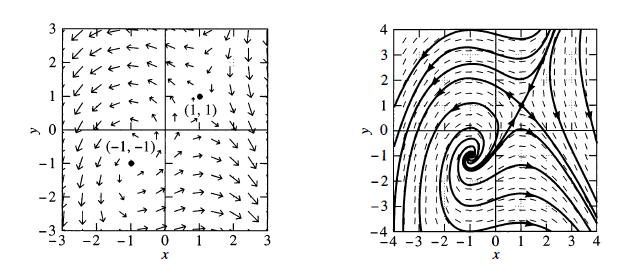
\includegraphics[width=15cm, height=6cm]{slope}
\end{center}
\captionof{figure}{En samling af linjeelementer(tv.) og et faseportæt(th.) til \eqref{DLS}. Figuren er taget fra \citep[s. 490]{EP}} \label{slope}
\hfill \break

\textnormal{På Figur \ref{slope} kan man se, hvordan løsningskurverne i faseportrættet følger linjeelementerne, og dermed også bevæger sig henholdsvis hen  imod eller væk fra ligevægtpunkterne.}

\end{Example}

\hfill \break
Vi karakteriserer ligevægtspunkter ud fra løsningskurvernes opførsel omkring dem. Givet et ligevægtspunkt $(x^*,y^*)$ i et autonomt system kaldes dette ligevægtspunkt således for en knude, såfremt følgende er gældene for løsningskurverne:
\begin{itemize}
    \item Enten går enhver løsningskurve mod ligevægtspunktet $(x^*,y^*)$ når $t \to + \infty$, eller også går enhver løsningskurve væk fra $(x^*,y^*)$ når $t \to + \infty$, og
    \item Enhver løsningskurve er tangent i $(x^*,y^*)$ til en lige linje igennem ligevægtspunktet.  
\end{itemize}
En knude kaldes en egentlig knude, hvis der ikke er et par af modsatliggende løsningskurver, der er tangent til den samme lige linje gennem $(x^*,y^*)$ og kaldes for en uegentlig knude, hvis dette ikke er tilfældet. Dette er illustreret i figur \ref{noder}.
\begin{figure} [H]
    \centering
    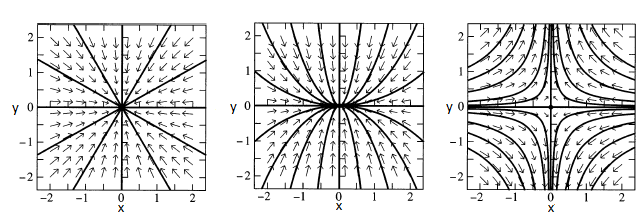
\includegraphics[scale=0.8]{Images/noder.png}
    \caption{En egentlig knude (tv.),en uegentlig knude (m) og et saddelpunkt (th.). Figuren er taget fra \citep[s. 491-492]{EP}}
    \label{noder}
\end{figure}

De to ligevægtspunkter til venstre i figur \ref{noder} kaldes også for dræn, da alle løsningskurverne går ind mod ligevægtspunktet. Hvis alle løsningskurverne går væk fra ligevægtspunktet, kaldes punktet en kilde.

Ligevægtspunktet yderst til højre i figur \ref{noder} kaldes et saddelpunkt. Et saddelpunkt er karakteriseret ved, at mindst en løsningskurve går mod $(x^*,y^*)$, at mindst en løsningskurve bevæger sig væk fra $(x^*,y^*)$ og, at de løsningskurver, der bevæger sig væk fra punktet, er ubegrænsede.
\\
En mere overordnet metode til beskrivelse af løsningskurvernes opførsel omkring et ligevægtspunkt, er ved brug af begrebet stabilitet.

\begin{definition}[Stabilitet af ligevægtspunkt]
Lad $\dot{y}(t)=\vec{f}(\vec{y(t)})$
være et autonomt differentialligningssystem, $\vec{y^*}=(y^*_{1},y^*_{2}, \cdots ,y^*_{n})$ et ligevægtspunkt og $\vec {y_0}=(y_{0,1},y_{0,2}, \cdots ,y_{0,n})$ et begyndelsespunkt. Ligevægtspunktet siges at være stabilt, såfremt der for ethvert $\varepsilon >0$ eksisterer et $\delta >0$ så følgende gælder:
$$|\vec y_0 - \vec {y^*}|< \delta \Rightarrow |\vec y(t) - \vec {y^*}| < \varepsilon, \\ \forall t > 0$$
\end{definition}
Et ligevægtspunkt kaldes ustabilt, hvis det ikke er stabilt.
Udover at være stabilt kan et ligevægtspunkt også være asymptotisk stabilt, hvilket vil sige, at det udover at være stabilt, også har egenskaben at alle løsningskurver tilstrækkelig tæt på ligevægtspunktet, vil bevæge sig ind mod ligevægtpunktet.

\begin{definition}[Asymptotisk stabilitet af ligevægtspunkt]
Lad 
$\dot{y}(t) = \vec{f}(\vec{y}(t))$
være et autonomt differentialligningssystem, $\vec {y^*}=(y_1^*,y_2^* \cdots ,y_n^*)$ et ligevægtspunkt og $\vec y_0=(y_{0,1},y_{0,2} \cdots ,y_{0,n})$ et begyndelsespunkt. Ligevægtspunktet siges at være asymptotisk stabilt, såfremt der eksisterer et $\delta >0$, så følgende gælder:
$$|\vec y_0 - \vec {y^*}|< \delta \Rightarrow \lim_{t\to\infty} \vec y(t)= \vec {y^*}$$
\end{definition}
Det ses således, at knuderne i figur \ref{noder} også kan beskrives som asymptotisk stabile ligevægtspunkter, mens saddelpunktet er ustabilt. \\
Et center er defineret ved, at alle løsningskurverne former lukkede kurver omkring centeret. Dette er et eksempel på et stabilt punkt, som ikke er asymptotisk stabilt, mens en spiral kan være enten asymptotisk stabil eller ustabil. Disse to tilfælde er illustreret i figur \ref{center}.

\begin{figure} [H]
    \centering
    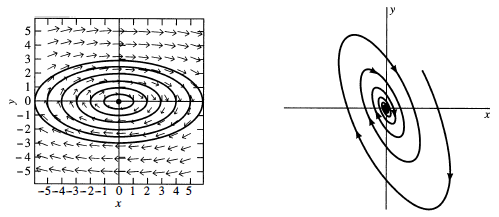
\includegraphics{Images/center.png}
    \caption{Et center (tv.) og en spiral (th.). Figuren er taget fra \citep[s. 493-495]{EP}}
    \label{center}
\end{figure}

\section{Stabilitets-analyse af system}
Dette afsnit samt underafsnit er baseret på \citep[afsnit 7.3]{EP} \\
Givet et autonomt system af differentialligninger,
\begin{equation}
\label{stab1}
    \begin{aligned}
    &\frac{dx}{dt}=F(x(t),y(t)),\\ 
    &\frac{dy}{dt}=G(x(t),y(t))
    \end{aligned}
\end{equation}
vil vi i dette afsnit undersøge, hvordan løsningerne opfører sig i nærheden af et isoleret ligevægtspunkt $(x^*,y^*)$. At et ligevægtspunkt er isoleret vil sige, at der i en omegn af ligevægtspunktet ikke eksisterer andre ligevægtspunkter. Det antages, at funktionerne $F$ og $G$ er kontinuerte og differentiable i en omegn af ligevægtspunktet.
Det kan antages uden tab af generalitet, at $x^*=y^*=0$. Dette kan med fordel antages, da vi
kun er interesseret i at sige noget om løsningskurvernes opførsel omkring ligevægtspunktet. Vi kan således omskrive systemet ved at sætte $u(t)=x(t)-x^*$ og $v(t)=y(t)-y^*$. Dermed bliver

\begin{equation*}
    \begin{aligned}
    &\frac{du}{dt}=\frac{dx}{dt}-\frac{dx^*}{dt}=\frac{dx}{dt}\\ 
    &\frac{dv}{dt}=\frac{dy}{dt}-\frac{dy^*}{dt}=\frac{dy}{dt},
    \end{aligned}
\end{equation*}

da $\frac{dx^*}{dt},\frac{dy^*}{dt}=0$. Systemet er dermed ækvivalent med det nye system:

\begin{equation}
\label{stab2}
    \begin{aligned}
    &\frac{du}{dt}=f(u(t),v(t)),\\ 
    &\frac{dv}{dt}=g(u(t),v(t))
    \end{aligned}
\end{equation}
hvor
\begin{equation*}
\begin{aligned}
&f(u,v)=F(u+x^*,v+y^*),\\ 
    &g(u,v)=G(u+x^*,v+y^*)
\end{aligned}
\end{equation*}
i den forstand at afbildningen, $(x(t),y(t)) \mapsto (u(t),v(t))$, definerer en bijektion af den ene løsningsmængde på den anden. Løsningskurverne for systemet $(\ref{stab1})$ er dermed lig løsningskurverne for $(\ref{stab2})$ efter koordinatskiftet $(u,v)\rightarrow(u+x^*,v+y^*)$. De to faseportrætter er altså identiske omkring de to ligevægtspunkter $(x^*,y^*)$ og $(0,0)$, som vist i figur (\ref{grafer}).
\begin{figure}[H]
    \centering
    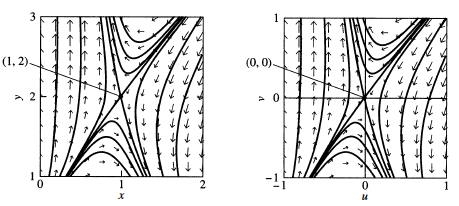
\includegraphics[scale=0.9]{grafer.png}
    \caption{System med ligevægtspunkt i $(1,2)$ i $x,y$-koordinatsystemet (th.) og det ækvivalente system i $u,v$-koordinatsystemet med ligevægtspunkt i $(0,0)$. Figuren er taget fra \citep[s. 501]{EP}}
    \label{grafer}
\end{figure}

\subsection{Linearisering}
Taylors formel for funktioner af to variable indebærer, at hvis funktionen $F(x,y)$ er kontinuert og differentiabel omkring punktet, $(x^*,y^*)$, så er jævnfør \citep[s. 501]{EP}:
\begin{equation*}
F(u+x^*,v+y^*)=F(x^*,y^*)+F_x(x^*,y^*)u+F_y(x^*,y^*)v+r(u,v),
\end{equation*}

hvor restledet $r(u,v)$ opfylder:
\begin{equation}
 \lim_{(u,v)\to (0,0)} \frac{r(u,v)}{\sqrt{u^2+v^2}}=0  
 \label{restled}
\end{equation}

Anvendes Taylors formel på funktionerne i det omskrevne system (\ref{stab2}), får vi funktionerne:

\begin{equation*}
    \begin{aligned}
    &F(u+x^*,v+y^*)=F(x^*,y^*)+F_x(x^*,y^*)u+F_y(x^*,y^*)v+r(u,v),\\ 
    &G(u+x^*,v+y^*)=G(x^*,y^*)+G_x(x^*,y^*)u+G_y(x^*,y^*)v+s(u,v),
    \end{aligned}
\end{equation*}
hvor $r(u,v)$ og $s(u,v)$  er restleddene. \\
Antag at, $(x^*,y^*)$, er et isoleret ligevægtspunkt. Så er,  $F(x^*,y^*)=G(x^*,y^*)=0$, og vi får:
\begin{equation*}
    \begin{aligned}
    &\frac{du}{dt}=F_x(x^*,y^*)u+F_y(x^*,y^*)v+r(u,v),\\ 
    &\frac{dv}{dt}=G_x(x^*,y^*)u+G_y(x^*,y^*)v+s(u,v)
    \end{aligned}
\end{equation*}

Da begge restled $r(u,v)$ og $s(u,v)$ opfylder ligning (\ref{restled}), vil vi altså, når $(u,v)$ er tæt på ligevægtspunktet $(0,0)$, få en tilnærmelse af det lineære system, som kan løses:

\begin{equation*}
    \begin{aligned}
    &\frac{du}{dt}=F_x(x^*,y^*)u+F_y(x^*,y^*)v,\\ 
    &\frac{dv}{dt}=G_x(x^*,y^*)u+G_y(x^*,y^*)v
    \end{aligned}
\end{equation*}
Dette lineariserede system vil således være en approksimation af det givne ikke-lineære system omkring ligevægtspunktet.
Det ses, at koefficienterne for $u$ og $v$ i det lineariserede system er henholdsvis $F_x(x^*,y^*),G_x(x^*,y^*)$ og $F_y(x^*,y^*),G_y(x^*,y^*)$. \\
Lineariseringen er altså givet ved:

\begin{equation*}
    \begin{aligned}
    &\frac{d\vec{u}}{dt}=\textbf{J}\vec{u}
    \end{aligned}
\end{equation*}
Hvor $\vec{u}=[u \ v]^T$ og $\textbf{J}$ er Jacobi-matricen for vektorfunktionen $(F,G)$ evalueret i ligevægtspunktet $(x^*,y^*)$. En Jacobi-matrix defineres ved:

\begin{definition}[Jacobi-matrix]
Lad $$\vec{f}: \mathbb{R}^n \to \mathbb{R}^m$$ være en funktion. \\ Da defineres en $m \times n$ matrix, $\textbf{J}$, på $\vec{f}$ til at være Jacobi-matricen til funktionen og skrives på formen:
$$\textbf{J}_{\vec{f}}(\vec{y}) = \frac{d\vec f}{d\vec{y}} =
\begin{bmatrix}
    \frac{\partial f_1}{\partial y_{1}} & \frac{\partial f_1}{\partial y_{2}} & \dots & \frac{\partial f_1}{\partial y_{n}} \\
    \frac{\partial f_2}{\partial y_{1}} & \frac{\partial f_2}{\partial y_{2}} & \dots & \frac{\partial f_2}{\partial y_{n}} \\
    \vdots & \vdots & \ddots & \vdots \\
    \frac{\partial f_m}{\partial y_{1}} & \frac{\partial f_m}{\partial y_{2}} & \dots & \frac{\partial f_m}{\partial y_{n}}
\end{bmatrix},$$
eller komponentvist:
$$\textbf{J}_{ij} = \frac{\partial f_i}{\partial y_j}$$

Jacobi-matricen er en lineær afbildning $\mathbb{R}^n \to \mathbb{R}^m$, der angiver en lineær approksimation af $\vec{f}$ til et $\vec{y}$.
\end{definition}

\subsection{Analyse af lineære systemer}\label{AnalLinSys}

Givet et lineært system af differentialligninger på formen,
$$\dot{y}(t) = A \vec{y}(t)$$
kan vi ved hjælp af egenværdierne for matricen $A$ analysere ligevægtspunkterne i systemet. \\ 
Givet et lineært system af differentialligninger i $\mathbb{R}^2$ findes egenværdierne, af koefficient matricen $A$, ved at løse den karakteristiske ligning:

\begin{equation}
 \det(A-\lambda I)= \begin{vmatrix}
a-\lambda & b \\
c & d -\lambda
\end{vmatrix}=(a-\lambda)(d-\lambda)-bc=0
\label{detA}
\end{equation}
Lad $(0,0)$ være et isoleret ligevægtspunkt, så vil $\det A$ være forskellig fra $0$, da ligevægtspunktet kun er isoleret, såfremt matricen $A$ er invertibel, og den homogene ligning dermed kun har den trivielle løsning $(0,0)$.\\
Dette betyder, at $\lambda=0$ ikke er en løsning i \eqref{detA}. Dermed er begge egenværdier for $A$ forskellige fra $0$.

De to egenværdier kan altså være:
\begin{itemize}
    \item Reelle og forskellige med samme fortegn
    \item Reelle og forskellige med forskelligt fortegn
    \item Reelle og ens
    \item Kompleks konjugerede med real-del forskellig fra 0
    \item  Rent imaginære
\end{itemize}

\subsubsection{Reelle og forskellige med samme fortegn}
I dette tilfælde har matricen $A$ to lineært uafhængige egenvektorer $\vec{v_1}$ og $\vec{v_2}$. Den fuldstændige løsning kan dermed skrives som:
$$\vec{y}(t)=c_1\vec{v_1}e^{\lambda_1 t}+c_2\vec{v_2}e^{\lambda_2 t}$$
Betragtes denne løsning i et $uv$-koordinatsystem med $\vec{v_1}$ og $\vec{v_2}$ som basisvektorer, som vist i figur \ref{uv-koordinatsystem}, vil en løsningskurve, som opfylder begyndelsesbetingelserne $u(0)=u_0$ og $v(0)=v_0$ kunne beskrives ved:
\begin{equation*}
    u(t)=u_0e^{\lambda_1 t} \ \  v(t)=v_0e^{\lambda_2 t}
\end{equation*}
\begin{figure}[H]
    \centering
    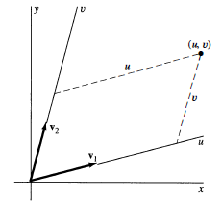
\includegraphics[scale=0.9]{uv-koordinatsystem.png}
    \caption{$u,v$-koordinatsystemet bestemt ved egenvektorerne $\vec{v_1}$ og $\vec{v_2}$ \citep[s. 503]{EP}}
    \label{uv-koordinatsystem}
\end{figure}
Hvis $v_0=0$ eller $u_0=0$ vil løsningskurven ligge på henholdsvis $u$-aksen og $v$-aksen. Hvis $u_0,v_0 \neq 0$ kan den parametriske kurve skrives på formen $v=Cu^k$. Dette ses ved følgende udregning:
\begin{equation*}
    u(t)=u_0e^{\lambda_1 t} \Rightarrow \ln \left(\frac{u(t)}{u_0} \right)=\lambda_1 t \Rightarrow t= \frac{\ln \left(\frac{u(t)}{u_0} \right)}{\lambda_1}
\end{equation*}
Foregående udregning kan foretages, da $u(t)$ og $u_0$ altid har samme fortegn, da $e^{\lambda_1 t} > 0$.
\begin{equation*}
v(t)=v_0e^{\lambda_2 t}=v_0e^{\lambda_2 \frac{\ln \left(\frac{u(t)}{u_0} \right)}{\lambda_1}} =  v_0\left(\frac{u(t)}{u_0}\right)^{\frac{\lambda_2}{\lambda_1}}
\end{equation*}
Altså er $v=Cu^k$, hvor $C=\frac{v_0}{u_0^{(\lambda_2 / \lambda_1)}}$ og $k=\frac{\lambda_2}{\lambda_1} > 0$, da egenværdierne har samme fortegn. \\
Da $v=Cu^k$ er en potensfunktion, vil løsningskurven være  tangent med $v$-aksen i $(0,0)$ for $k>1$, og for $0<k<1$ er den tangent med $u$-aksen. $(0,0)$ er derfor en uegentlig knude. Hvis egenværdierne er positive, vil løsningskurverne bevæge sig væk fra ligevægtspunktet, når $t \to \infty$. $(0,0)$ er derfor en kilde i dette tilfælde. Det modsatte gør sig gældende, hvis begge egenværdier er negative, i hvilket tilfælde $(0,0)$ vil være et dræn.
\subsubsection{Reelle og forskellige med forskelligt fortegn}
Som i forrige tilfælde kan løsningskurverne bestemmes ved:
\begin{equation*}
    u(t)=u_0e^{\lambda_1 t} \ \  v(t)=v_0e^{\lambda_2 t}
\end{equation*}
Forskellen er nu bare at $\lambda_2<0<\lambda_1$. Løsningskurverne, hvor $u_0,v_0 \neq 0$, kan som før skrives på formen $v=Cu^k$, hvor forskellen er, at $k=\frac{\lambda_2}{\lambda_1}<0$. Løsningskurverne vil derfor være hyperbler, og ligevægtspunktet er dermed ustabilt.
\subsubsection{Reelle og ens}
I dette tilfælde afhænger opførslen af løsningskurverne omkring ligevægtspunktet af, om $A$-matricen har to lineært uafhængige egenvektorer. Hvis dette er tilfældet kan løsningskurverne som før beskrives ved $v=Cu^k$ i $uv$-koordinatsystemet, hvor $k=1$ i dette tilfælde. Vi får dermed $v=Cu$, og løsningskurverne ligger altså på en lige linje gennem origo. Ligevægtspunktet vil derfor være en egentlig knude. Hvis $\lambda>0$ er punktet en kilde, og hvis $\lambda<0$ er punktet et dræn. \\
Hvis $A$-matricen ikke har to lineært uafhængige egenvektorer, har systemet to lineært uafhængige løsninger:
\begin{equation*}
    \vec{y_1}(t)=\vec{v_1}e^{\lambda t} \ \textnormal{og} \ \vec{y_2}(t)=(\vec{v_1}t+\vec{v_2})e^{\lambda t}
\end{equation*}
Og dermed den fuldstændige løsning:
\begin{equation*}
    c_1\vec{y_1}(t)+c_2\vec{y_2}(t) = \\
    (c_1+c_2t)\vec{v_1}e^{\lambda t} +c_2\vec{v_2}e^{\lambda t}
\end{equation*}
Hvor $\lambda$ er systemets egenværdi med tilhørende egenvektore $\vec{v_1}$, og $\vec{v_2}$, som opfylder $(A-\lambda I)\vec{v_2}=\vec{v_1}$.
Som før kan løsningskurverne beskrives i et $uv$-koordinatsystem bestemt af $\vec{v_1}$ og $\vec{v_2}$. Løsningskurverne kan altså beskrives ved:
\begin{equation*}
    v(t)=v_0e^{\lambda t}, \ u(t)=(u_0+v_0t)e^{\lambda t}
\end{equation*}
Hvor $v_0=v(0)$ og $u_0=u(0)$. Hvis $v_0=0$ ligger løsningskurven på $u$-aksen. Ellers gælder følgende for løsningskurven:
\begin{equation*}
    \frac{dv}{du}=\frac{\frac{dv}{dt}}{\frac{du}{dt}}=\frac{\lambda v_0e^{\lambda t}}{v_0e^{\lambda t}+\lambda(u_0+v_0t)e^{\lambda t}}=\frac{\lambda v_0}{v_0+\lambda(u_0+v_0t)}
\end{equation*}
Det ses at $\frac{dv}{du} \to 0$ nåt $t \to \pm
\infty$. Altså er enhver løsningskurve tangent med $u$-aksen. $(0,0)$ er derfor en uegentlig knude. Den er en kilde, hvis $\lambda>0$ og et dræn, hvis $\lambda<0$.
\subsubsection{Kompleks konjugerede med real-del forskellig fra 0}
Hvis systemet har to komplekst konjugerede egenværdier $\lambda = p+qi$ og $\bar{\lambda}=p-qi$, (hvor $p,q \neq 0$) med tilhørende komplekst konjugerede egenvektorer $\vec{v}=\vec{a}+\vec{b}i$ og $\bar{\vec{v}}=\vec{a}-\vec{b}i$. Så har systemet to uafhængige løsninger:
\begin{equation*}
    \vec{y_1}(t)=e^{pt}(\vec{a}\cos(qt)-\vec{b}\sin(qt)) \ \textnormal{og} \ \vec{y_2}(t)=e^{pt}(\vec{b}\cos(qt)+\vec{a}\sin(qt))
\end{equation*}
Den fuldstændige løsning er altså givet ved:
\begin{equation*}
    \vec{y}(t)=c_1e^{pt}(\vec{a}\cos(qt)-\vec{b}\sin(qt))+c_2e^{pt}(\vec{b}\cos(qt)+\vec{a}\sin(qt))
\end{equation*}
Hvilket kan omskrives til:
\begin{equation*}
    \vec{y}=\begin{bmatrix}
        \vec{a} & \vec{b}
    \end{bmatrix} \begin{bmatrix}
        \cos(qt) & \sin(qt) \\
        -\sin(qt) & \cos(qt)
    \end{bmatrix} \begin{bmatrix}
        c_1e^{pt} \\
        c_2e^{pt}
    \end{bmatrix}
\end{equation*}
Hvis $p<0$ vil  $c_1e^{pt},c_2e^{pt} \to 0$ når $t \to +\infty$. Da vektoren $\begin{bmatrix}
        c_1e^{pt} \\
        c_2e^{pt}
    \end{bmatrix}$ ganges på en rotationsmatrix, er $(0,0)$ i dette tilfælde et spiral dræn. Hvis $p>0$, vil ligevægtspunktet være en spiral kilde. Dette skyldes, at vi får en cirkel, for $t$ gennemløbende $[0,\frac{2\pi}{q}]$, hvis $e^{pt}$ udelades fra formlen. 
\subsubsection{Rent imaginære}
Hvis systemet har kompleks konjugerede egenværdier $\lambda=qi$ og $\bar{\lambda}=-qi$ med tilhørende kompleks konjugerede egenvektorer $\vec{v}=\vec{a}+\vec{b}i$ og $\bar{\vec{v}}=\vec{a}-\vec{b}i$. Så har systemet samme løsning som i forrige afsnit, hvor $p=0$:
\begin{equation*}
    \vec{x}(t)=c_1(\vec{a}\cos(qt)-\vec{b}\sin(qt))+c_2(\vec{b}\cos(qt)+\vec{a}\sin(qt))
\end{equation*}
Som før kan dette omskrives til:
\begin{equation*}
    \vec{x}(t)=\begin{bmatrix}
        \vec{a} & \vec{b}
    \end{bmatrix} \begin{bmatrix}
        \cos(qt) & \sin(qt) \\
        -\sin(qt) & \cos(qt)
    \end{bmatrix} \begin{bmatrix}
        c_1\\
        c_2
    \end{bmatrix}
\end{equation*}
Vi kan omskrive udtrykket for $\vec{x}(t)$ ved først at lave to omskrivninger af udtrykkende $c_1\cos(qt)+c_2\sin(qt)$ og $-c_1\sin(qt)+c_2\cos(qt)$:
\begin{equation*}
    c_1\cos(qt)+c_2\sin(qt)=\begin{pmatrix}
        c_1 \\ c_2
    \end{pmatrix} \cdot \begin{pmatrix}
        \cos(qt) \\ \sin(qt) 
    \end{pmatrix}  = \sqrt{c_1^2+c_2^2}\begin{pmatrix}
        \frac{c_1}{\sqrt{c_1^2+c_2^2}}\\ \frac{c_2}{\sqrt{c_1^2+c_2^2}}
    \end{pmatrix} \cdot \begin{pmatrix}
        \cos(qt) \\ \sin(qt) 
    \end{pmatrix}
\end{equation*}
Da $\begin{pmatrix}
        \frac{c_1}{\sqrt{c_1^2+c_2^2}}\\ \frac{c_2}{\sqrt{c_1^2+c_2^2}}
    \end{pmatrix}$ er en enhedsvektor, kan vi omskrive til følgende:
\begin{equation*}
\sqrt{c_1^2+c_2^2}\begin{pmatrix}
        \frac{c_1}{\sqrt{c_1^2+c_2^2}}\\ \frac{c_2}{\sqrt{c_1^2+c_2^2}}
    \end{pmatrix} \cdot \begin{pmatrix}
        \cos(qt) \\ \sin(qt) 
    \end{pmatrix}=
     \sqrt{c_1^2+c_2^2}\begin{pmatrix}
        \cos(\alpha)\\ 
        \sin(\alpha)
    \end{pmatrix} \cdot \begin{pmatrix}
        \cos(qt) \\ \sin(qt) 
    \end{pmatrix}
\end{equation*}
Da $\vec{a} \cdot \vec{b}= ||\vec{a}|| \ ||\vec{b}||\cos(\theta)$, hvor $\theta$ er vinklen mellem de to vektorer, får vi: 
\begin{equation*}
    \sqrt{c_1^2+c_2^2}\begin{pmatrix}
        \cos(\alpha)\\ 
        \sin(\alpha)
    \end{pmatrix} \cdot \begin{pmatrix}
        \cos(qt) \\ \sin(qt) 
    \end{pmatrix}=\sqrt{c_1^2+c_2^2}\cos(qt-\alpha)
\end{equation*} 
På samme måde kan vi finde et udtryk for $-c_1\sin(qt)+c_2\cos(qt)$, men udregningerne vil ikke blive gennemgået igen. Vi får udtrykket:
\begin{equation*}
    -c_1\sin(qt)+c_2\cos(qt)= \sqrt{c_1^2+c_2^2}\sin(qt-\alpha)
\end{equation*}
Vi kan nu udtrykke $\vec{x}(t)$ som følger:
\begin{equation*}
    \vec{x}(t)=\sqrt{c_1^2+c_2^2}\cos(qt-\alpha)\vec{a}+\sqrt{c_1^2+c_2^2}\sin(qt-\alpha)\vec{b}
\end{equation*}
\\
Det ses altså, at i dette tilfælde vil løsningskurven være en ellipse med $(0,0)$ som centrum, da vektorerne $\vec{a}$ og $\vec{b}$ ikke har samme længde. Dermed er $(0,0)$ et stabilt centrum i dette tilfælde. \\

Ovenstående afsnit opsummeres i en tabel: 

\begin{table} [H]
\centering 
    \begin{tabular}{|l|l|l|}
    \hline
    \textbf{Egenværdier}                                    & \textbf{Type af ligevægtspunkt}            & \textbf{Stabilitet}          \\ \hline
    $\lambda_1 > \lambda_2 > 0$                     & Uegentlig kilde                   & Ustabilt            \\ \hline
    $\lambda_1 < \lambda_2 < 0$                     & Uegentlig dræn                    & Asymptotisk stabilt \\ \hline
    $\lambda_1 < 0 < \lambda_2$                     & Saddelpunkt                       & Ustabilt            \\ \hline
    $\lambda_1 = \lambda_2 > 0$                     & Egentlig eller uegentlig kilde    & Ustabilt            \\ \hline
    $\lambda_1 = \lambda_2 < 0$                     & Egentlig eller uegentlig dræn     & Asymptotisk stabilt \\ \hline
    $\lambda_1, \lambda_2 =p \pm qi, p > 0$         & Spiralkilde                       & Ustabilt            \\ \hline
    $\lambda_1, \lambda_2 =p \pm qi, p < 0$         & Spiraldræn                        & Asymptotisk stabilt \\ \hline
    $\lambda_1, \lambda_2 = \pm qi, q > 0$          & Centrum                           & Stabilt             \\ \hline
    \end{tabular}
\caption{Sammenhæng mellem egenværdier og ligevægtspunkter}\label{tab:egenvardi}
\end{table}

\textbf{Bemærk} at jævnfør \citep[s. 738]{FDEB}, vil tabellen for egenværdierne for et lineariseret system være den samme, dog med undtagelse af de tilfælde hvor egenværdierne er reelle og ens, eller rent imaginære. For tilfældet hvor egenværdierne er reelle og ens vil løsningskurverne ligeledes kunne danne spiralpunkt. I tilfældet hvor egenværdierne er rent imaginære vil ligevægtspunktet være et centrum eller spiralpunkt og være enten stabilt, ustabilt eller asymptotisk stabilt. For det lineariserede system, i form af Jacobi-matricen, vil det altså ikke være tilstrækkeligt at benytte egenværdierne til at beskrive ligevægtspunktet. I disse tilfælde vil der i projektet anvendes Lyapunov-funktioner for yderligere analyse af stabiliteten af ligevægtspunktet.




\section{Nulkliner}
Dette afsnit er baseret på Afsnit 9.1 i \citep{Hirsch} \\
Når vi skal analysere et ikke-lineært system som Lotka-Volterra modellen, er bestemmelsen af nulkliner et nyttigt redskab.

\begin{definition}[Nulkliner]
Lad 
\\
$$\dot{y} = \frac{d\vec{y}}{dt} = 
\begin{bmatrix}
\frac{dy_1}{dt} \\
\frac{dy_2}{dt}\\
\vdots \\
\frac{dy_n}{dt}
\end{bmatrix}
=
\begin{bmatrix}
f_1(t, y_1, y_2, \hdots, y_n)\\
f_2(t, y_1, y_2, \hdots, y_n)\\
\vdots \\
f_n(t, y_1, y_2, \hdots, y_n)
\end{bmatrix}$$
\\
være et differentialligningssystem. \\
$y_j$-nulklinen er mængden af punkter, hvor $\frac{dy_j}{dt}=0$ 
\end{definition}
Det ses, at de steder hvor alle nulklinerne skærer hinanden, er systemets ligevægtspunkter. \\
Har man fundet alle nulklinerne for et system i $\mathbb{R}^n$, deler disse nulkliner sædvanligvis $\mathbb{R}^n$ op i regioner, hvor $y_j$-komponenterne i vektorfeltet peger i enten positiv eller negativ retning. \\
Ser vi på et førsteordens differentialligningssystem bestående af to funktioner, kan vi nemmere illustrere nulklinernes anvendelse.
\begin{Example}\textnormal{Fra \citep{Hirsch}}\\
\textnormal{Givet differentialligningssystemet:}
\begin{align*}
    x'&=y-x^2 \\
    y'&=x-2
\end{align*}
\textnormal{$x$-nulklinen er parablen $y=x^2$ og $y$-nulklinen er den vertikale linje $x=2$. De to nulkliner skærer hinanden i punktet $(2,4)$. Nulklinerne deler $\mathbb{R}^2$ op i 4 regioner $A,B,C,D$ som vist i figur \ref{nulkliner}. Når først vi har fået delt $\mathbb{R}^2$ i regioner kan vektorfeltets generelle retning i hver af disse regioner nu bestemmes. Dette gøres ved at vælge et tilfældigt punkt i hver region, og udregne vektorfeltets retning i dette punkt. Da det kun er på nulklinerne at vektorfeltet er parallelt med enten første- eller andenaksen vil vinklerne for alle vektorer i hver region tilhøre et bestemt af følgende åbne intervaller: $(0-\frac{\pi}{2}),(\frac{\pi}{2},\pi),(\pi,-\frac{\pi}{2}),(-\frac{\pi}{2},0)$. Punktet $(1,2)$ ligger i region A i figur \ref{nulkliner}(a). I dette punkt har vektorfeltet retningen $(1,-2)$, hvilket betyder at vinklerne for alle vektorerne i denne region ligger i intervallet $(-\frac{\pi}{2},0)$.  }

\begin{figure} [H]
    \centering
    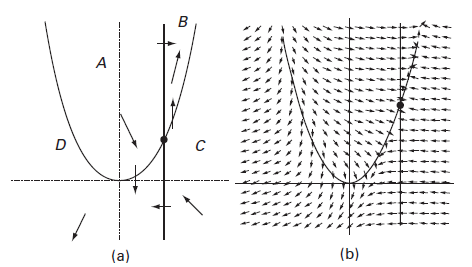
\includegraphics[scale=0.8]{Images/nulkliner.png}
    \caption{Nulklinerne og vektorfeltet for systemet}
    \label{nulkliner}
\end{figure}
\end{Example}




\section{Liapunov funktioner}



%\chapter*{...}

\begin{definition}[Punktfølge]
En punktfølge består af uendeligt mange nummererede elementer i $\mathbb{R}^2$:

\begin{equation}
    x^1, x^2, \hdots, x^k, \hdots
\end{equation}
\end{definition}

\begin{definition}[Konvergens punktfølge]
En punktfølge $\{x^k\}^\infty_{k=1}$ i $\mathbb{R}^n$ siges at være konvergent, hvis der eksisterer et punkt $x \in \mathbb{R}^n$ således, at 

\begin{equation}
    \lim_{k \to \infty} ||x-x^k|| = 0.
\end{equation}

I så fald kaldes $x$ for følgens grænsepunkt, grænsevektor, eller grænseværdi, vi siger, at punktfølgen konvergerer mod $x$, og vi skriver

\begin{equation}
    x^k \to x \ for \ k \to \infty \ eller \ \lim_{k \to \infty} x^k = x. 
\end{equation}

En punktfølge, der ikke er konvergent, siges at være divergent. 

\end{definition}

\begin{definition}[]
En punktfølge $\{x^k\}^\infty_{k=1}$ siges at være begrænset, hvis der eksisterer et positivt reelt tal $M$, så $||x^k|| \leq M$ for alle $k\in \mathbb{N}$. 
\end{definition}

\begin{mytheo}{}
h
\begin{enumerate}[label=(\alph*)]
    \item En punktfølge kan højst have et grænsepunkt. 
    \item Hvis en punktfølge er konvergent, er den begrænset. 
    \item Lad $\{x^k\}^\infty_{k=1}$ være en punktfølge $x$ et punkt i $\mathbb{R}^n$. Så gælder
    
    \begin{equation}
        x^k \to x \ for \ k \to \infty \Leftrightarrow x^k-x \to 0 \ for \ k \to \infty.
    \end{equation}
    
    \item Lad $\{x^k\}^\infty_{k=1}$ være en punktfølge. Så gælder
    
    \begin{equation}
        x^k \to 0 \ for \ k \to \infty \Leftrightarrow ||x^k|| \to 0 \ for \ k \to \infty.
    \end{equation}
    
\end{enumerate}

\end{mytheo}


\begin{mytheo}{Regneregler for grænseværdier}{dd}

\begin{enumerate}[label=(\alph*)]
    \item Hvis punktfølgen $\{x^k\}^\infty_{k=1}$ er konvergent, så er talfølgen $\{||x^k||\}^\infty_{k=1}$ konvergent, og 
    \begin{equation}
        \lim_{k \to \infty} ||x^k|| = || \lim_{k \to \infty} x^k||.
    \end{equation}
    
    \item Hvis punktfølgerne $\{x^k\}^\infty_{k=1}$ og $\{y^k\}^\infty_{k=1}$ er konvergente, så er punktfølgerne \\
    $\{x^k \pm y^k\}^\infty_{k=1}$ konvergente, og 
    
    \begin{equation}
        \lim_{k \to \infty} (x^k \pm y^k) =  \lim_{k \to \infty} x^k \pm \lim_{k \to \infty} y^k
    \end{equation}
    
    \item Hvis $\{a_k\}^\infty_{k=1}$ er en konvergent talfølge og $\{x^k\}^\infty_{k=1}$ er en konvergent punktfølge, så er punktfølgen $\{a_kx^k\}^\infty_{k=1}$ konvergent, og 
    
    \begin{equation}
        \lim_{k \to \infty} a_k x^k =  \lim_{k \to \infty} a_k \lim_{k \to \infty} x^k
    \end{equation}
    
    \item Hvis punktfølgerne $\{x^k\}^\infty_{k=1}$ og $\{y^k\}^\infty_{k=1}$ er konvergente, så er talfølgen $\{\langle x^k,y^k\rangle\}^\infty_{k=1}$ konvergent, og der gælder 
    
    \begin{equation}
         \lim_{k \to \infty} \langle x^k,y^k\rangle =   \langle \lim_{k \to \infty} x^k, \lim_{k \to \infty} y^k \rangle.
    \end{equation}
    
\end{enumerate}

\end{mytheo}
\section{Analyse af Lotka-Volterra's rovdyr-byttedyr model}
Vi benytter Laplacetransformation, hvis vi har begyndelsesværdier, da problemet kan reduceres til algebra (Se sidst i afsnittet for laplacetransformen af Lotka-Volterra):
\begin{Example}
\textnormal{Lad os betragte følgende system af ODEs med begyndelsesværdier, $x(0)=1$ og $y(0)=0$.}
\begin{align}
    2x' + y' - y &= t\\
    x' + y' &= t^2
\end{align}
\textnormal{Vi tager laplacetransfomationen af alt}
\begin{align*}
    2(s X(s) - x(0)) + sY(s) - y(0) - Y(s) &= \frac{1}{s^2}\\
    s X(s) - x(0) + sY(s) - y(0) &= \frac{2}{s^3}\\
    2sX(s) + (s-1)Y(s) &= 2 + \frac{1}{s^2}\\
    sX(s) + sY(s) &= 1 + \frac{2}{s^3}
\end{align*}
\textnormal{Det er klart, at $X(s)$ nemt kan fjernes. Så det gør vi}
\begin{align*}
    2sX(s) + (s-1)Y(s) &= 2 + \frac{1}{s^2}\\
    -2(sX(s) + sY(s) &= 1 + \frac{2}{s^3})\\
    (s-1-2s)Y(s) &= \frac{1}{s^2} - \frac{4}{s^3}\\
    (-s-1)Y(s) &= \frac{s-4}{s^3}\\
    Y(s) &= \frac{4-s}{s^3(s + 1)}
\end{align*}
\textnormal{Vi omskriver nu til flere brøker (Ved ikke hvad partial fractions hedder på dansk)}
$$ \frac{4-2}{s^3(s+1)} = \frac{A}{s} + \frac{B}{s^2} + \frac{C}{s^3} + \frac{D}{s+1}$$
\textnormal{Der ganges igennem med $s^3(s+1)$}
$$ 4 - s = A s^2(s+1) + Bs(s+1) + C(s+1) + Ds^3$$
\textnormal{Kigger nu på ligningen og indser, at}
\begin{align*}
    A + D &= 0\\
    A + B &= 0\\
    B + C &= -1\\
    C &= 4
\end{align*}
\textnormal{Da får vi: $B = -5$, $A = 5$, $D = -5$}
$$Y(s) = \frac{5}{s} -\frac{5}{s^2} + \frac{4}{s^3} - \frac{5}{s+1}$$
\textnormal{Da anvender vi $\mathcal{L}^{-1}$}
$$ y(t) = 5 - 5t + 2t^2 - 5e^{-t}$$
\textnormal{vi isolerer nu X(s) og tager $\mathcal{L}^{-1}$ i den laplacetransformerede ligning 3.2}
\begin{align*}
    s(X)s - 1 + sY(s) &= \frac{2}{s^3}\\
    X(s) &= \frac{1}{s} + \frac{s}{s^4} - Y(s)\\
    x(t) &= 1 + \frac{1}{3}t^3 - (5 - 5t + 2t^2 - 5e^{-t})\\
    x(t) &= -4 + 5t-2t^2 + \frac{1}{3}t^3 + 5e^{-t}
\end{align*}

\end{Example}


For vores tilfælde kan vi se følgende:

\begin{equation*}
    \dfrac{db}{dt}(t) = (H-Ir(t)) b(t), 
\end{equation*}

\begin{equation*}
    \dfrac{dr}{dt}(t) = (Jb(t)-K) r(t),
\end{equation*}

$$b' - (H - Ir)b = 0 $$
$$r' - (Jb - K)r = 0 $$
Ved at tage laplacetransformen fås:
$$sB(s) - b(0) - (\frac{H}{s} - \frac{I}{s}R(s))B(s) = 0$$
$$sR(s) - r(0) - (\frac{J}{s}B(s) - \frac{K}{s})R(s) = 0$$
Så vi skal bruge nogle begyndelsesværdier ellers er vi fanget :O

\subsection{Logistisk vækst af Lotka-Volterra's model}

Hvis vi ser på systemet:
\begin{align*}
    b' &= hb - ibr\\
    r' &= jbr - kr
\end{align*}
Dette skal omskrives til et problem med logistisk vækst med hensyn til byttedyrspopulationen, hvor vi ved, at følgende udtryk skal indgå:
$$b' = pb(1 -  \frac{b}{k}),$$
hvor $k$ er en konstant, der angiver, hvor meget føde, der er tilgængelig for byttedyrene, og $p$ er en proportionalitetskonstant.
\hfill \break
I Lotka-Volterra's model illustrerer første led i øverste ligning byttedyrets population ganget med en fødselsratekonstant. Dette ændres til følgende:
\begin{align*}
    b' & = pb(1 -  \frac{b}{k}) - ibr\\
    &\Updownarrow\\
    b' &= (p(1 - \frac{b}{k}) - ir)b
\end{align*}
Da har vi et nyt system med logistisk vækst:
\begin{align*}
    b' &= pb(1 - \frac{b}{k}) - ibr\\
    r' &= jbr - kr
\end{align*}


\chapter{Logistisk vækst af Lotka-Volterra's model}
I det tilfælde hvor byttedyrene, i Lotka-Volterra's model, har begrænset føde vil systemet bestå af differentialligninger med logistisk vækst. I det følgende vil logistisk vækst derfor blive forklaret.\\
\hfill \break

\section{Logistisk vækst}\label{lovaeg}
Hvis man forestiller sig at der ingen rovdyr er, da vil differentialligningen for byttedyr vokse eksponentielt, hvilket vil resultere i at antallet af byttedyrerne vil vokse uendeligt. Derfor tilføjes der en faktor for begrænset føde, så differentialligningen bliver på formen:

\begin{equation}\label{logvivp}
    \begin{cases}
    x'(t)&=ax(t)-bx(t)^2\\
    x(t_0)&=x_0
    \end{cases}
\end{equation}

Dette er en separabel differentialligning, og udfra dette kan vi tilføje en hjælpefunktion 
\begin{equation*}
    p(x)=ax-bx^2=ax\left(1-\frac{b}{a}x\right)
\end{equation*}
Ved faktorisering af $p(x)$ findes de værdier, hvor funktionen $x'(t)$ er lig $0$:
\begin{equation}
p(x)=0 \Leftrightarrow
    \begin{cases}
    &x_0 = 0,\\ 
    &x_0 = \frac{a}{b}
    \end{cases}
\end{equation}.

\begin{figure} [H]
    \centering
    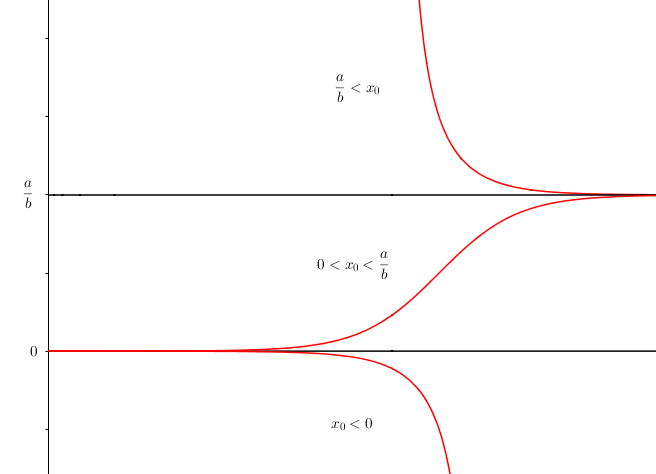
\includegraphics[scale=0.5]{Images/logi.png}
    \caption{Logistisk vækst}
    \label{logi}
\end{figure}

Ovenstånde figur illustrerer konklusionen af den kommende analyse for løsningskurver. Udfra den foregående faktorisering, vil der fremkomme fire mulige tilfælde for udseendet af løsningskurven til $t_0, x_0$:
\begin{enumerate}
    \item $x_0 = \frac{a}{b}, \ \textnormal{eller} \ x_0 = 0$ \\
    \item $0 < x_0 < \frac{a}{b}$\\
    \item $x_0 > \frac{a}{b}$ \\
    \item $x_0 < 0$ \\
\end{enumerate}
Tilfældene regnes nu igennem.

\subsubsection{Tilfælde 1}
Intuitivt ses det, at for tilfælde 1 vil tangenten være parallel med førsteaksen, og dermed vil løsningen gennem $(t_0, x_0)$ være konstant lig $x_0$. Grundet EES \citep{EES} er løsningen entydig. 
Altså har vi enten $x(t) \equiv \frac{a}{b}$ eller $x(t) \equiv 0$.\\
Vi giver her et argument for, at EES kan anvendes på det givne IVP \eqref{logvivp}.\\

\begin{enumerate}
    \item Funktionen $p(x)=ax-bx^2$ er defineret på hele $\mathbb{R}$ og afbilleder ind i $\mathbb{R}$. Dermed er $p \colon \mathbb{R}\times \mathbb{R}\to \mathbb{R}$.
    \item Hjælpefunktionen $p$ er kontinuert og differentiabel. Da eksisterer de partielle afledte, hvor $p'(x)=a-2bx$, som klart er kontinuert, da $p'(x)$ er et førstegradspolynomium.\\
    \item Det er trivielt opfyldt, da definitionsmængden er hele $\mathbb{R} \times \mathbb{R}$.\\ 
\end{enumerate}
Pér lemma \ref{th:LMD}, findes en løsning, $\phi(t)$, defineret på det maksimale definitionsinterval $]-\infty,\infty [$.

\subsubsection{Tilfælde 2}
Løsningskurven vil ligge i intervallet $\left] 0, \frac{a}{b} \right[$. Her vil den være være positiv og antage lokalt maksimum mellem $0$ og $\frac{a}{b}$.
Under følgende udregninger vil vi møde
\begin{equation*}
  \frac{1}{p(x)}=\frac{1}{ax-bx^2},
\end{equation*} 
hvor det er nødvendigt at finde dets stamfunktion. Her laves stambrøkdekomponering:

\begin{equation*}
    \frac{1}{ax(1-\frac{b}{a}x)}=\frac{A}{ax}+\frac{B}{1-\frac{b}{a}x}
\end{equation*}

For at finde værdierne, $A$ og $B$, sætter man på fælles brøkstreg:

\begin{equation*}
    \frac{A \left(1- \frac{b}{a}x \right)+Bax}{ax \left(1- \frac{b}{a}x \right)} =\frac{A + x \left( Ba-A \frac{b}{a} \right)}{ax \left(1-\frac{b}{a}x \right)}.
\end{equation*}

Udfra:
\begin{equation*}
\frac{1\cdot x^0+0\cdot x^1}{ax(1-\frac{b}{a}x)}
\end{equation*}

ses det, at $A=1$, og dermed er 
\begin{equation*}
    Ba - A \frac{b}{a} = 0 \Rightarrow B = \frac{1}{a} \cdot \frac{b}{a}.   
\end{equation*}

Da er 
\begin{align*}
    \frac{1}{p(x)} &= \frac{1}{ax}+\frac{\left( \frac{1}{a} \cdot \frac{b}{a} \right)}{1-\frac{b}{a}x} \\
    &= \frac{1}{ax \left( 1-\frac{b}{a}x \right)}
\end{align*}

Udfra foregående stambrøkskomponering kan vi udregne stamfunktionen, $H(x)$, til $\frac{1}{p(x)}$, jævnfør sætning \ref{th:LSD}:

\begin{align*}
    \int \frac{1}{ax}+\frac{ \frac{1}{a} \frac{b}{a}}{1-\frac{b}{a}x}dx
    &=\frac{1}{a}\ln|x|+\frac{\frac{1}{a}\frac{b}{a}}{-\frac{b}{a}}\ln \left|1-\frac{b}{a}x\right|\\
    &=\frac{1}{a}\ \ln|x|-\frac{1}{a}\ln \left|1-\frac{b}{a}x\right|
\end{align*}

Ved separation af $x'(t)$ i \eqref{logvivp} fås:
\begin{equation*}
    \frac{1}{(ax(t)-bx(t)^2)} x'(t)= 1   
\end{equation*}

Vi integrerer fra $t_0$ til $t$:
\begin{align*}
    \int^t_{t_0} \frac{1}{(ax(s)-bx(s)^2)} x'(s)ds&=\int^{t}_{t_0}1\ ds\\
    \left[ \frac{1}{a} \ln \left| \frac{x(s)}{1-\frac{b}{a}x(s)} \right| \right]^t_{t_0}&=[s]^t_{t_0}\\
    \frac{1}{a}\ln \left|\frac{x(t)}{1-\frac{b}{a}x(t)} \right|-\frac{1}{a}\ln \left| \frac{
    x_0}{1-\frac{b}{a}x_0} \right|&=t-t_0\\
    \ln \left| \frac{x(t)}{1-\frac{b}{a}x(t)}\right|-\ln \left|\frac{x_0}{1-\frac{b}{a}x_0}\right| &=a(t-t_0).
\end{align*}

Nu udredes, hvad $x(t)$ er, ved brug af logaritme regnereglerne:

\begin{equation*}
    \ln \left| \frac{x(t)}{x_0} \cdot \frac{1-\frac{b}{a}x_0}{1-\frac{b}{a}x(t)} \right| = a(t-t_0)
\end{equation*}

\begin{equation}\label{nur}
    \left|\frac{x(t)}{x_0}\right| \cdot \left| \frac{1-\frac{b}{a}x_0}{1-\frac{b}{a}x(t)} \right| 
    = e^{a(t-t_0)}
\end{equation}

For at fjerne de numeriske tegn ses der på, hvilken værdi de to brøker vil antage. Den første brøk vil blive positiv, da $\frac{a}{b}>x_0>0$, hvormed $x(t)>0$. Ses der på den anden brøk, vil også denne blive positiv, da $\frac{b}{a}x_0<\frac{b}{a}\frac{a}{b}=1$. \\
\hfill 
Da fjernes de numeriske tegn, og der isoleres for $x(t)$:

$$x(t) = \frac{x_0}{1 - \frac{b}{a}x_0} \left(1- \frac{b}{a}x(t) \right)e^{a(t-t_0)}$$

Nu sættes $K = \frac{x_0}{1 - \frac{b}{a}x_0}$:

\begin{align*}
x(t) &= K e^{(a(t-t_0))}-K \frac{b}{a}x(t) e^{a(t-t_0)} \\
\left(1+K \frac{b}{a} e^{a(t-t_0)}\right)x(t) &=K e^{a(t-t_0)} \\
x(t) &=\frac{K e^{a(t-t_0)}}{1+K \frac{b}{a} e^{a(t-t_0)}} = \frac{K e^{a(t-t_0)}}{K e^{a(t-t_0)}}\frac{1}{\frac{b}{a}+\frac{1}{Ke^{a(t-t_0)}}} \\
&= \frac{1}{\frac{b}{a}+(Ke^{a(t-t_0)})^{-1}} = \frac{1}{\frac{b}{a}+K^{-1}e^{-a(t-t_0)}} \\
&=\frac{1}{\frac{b}{a}+ \left( \frac{1-\frac{b}{a}x_0}{x_0} \right)e^{-a(t-t_0)}} \\
&=\frac{x_0}{ \left(1-\frac{b}{a}x_0 \right)e^{-a(t-t_0)}+ \frac{b}{a}x_0 }
\end{align*}

Da er $x(t)$ en løsning, som antager værdier i intervallet, $]0, \frac{a}{b}[.$

\subsubsection{Tilfælde 3}
Løsningskurven for dette tilfælde vil ligge i $\left] \frac{a}{b}, +\infty \right[$ og vil dermed være positiv.\\
\hfill \break
Dette tilfælde, samt tilfælde 4, vil følge en analog proces op til og med integrationen i \eqref{nur}.\\
\hfill \break

Det ønskes igen at fjerne de numeriske tegn. Det er givet, at $x_0 > \frac{a}{b}$, hvormed $x(t) > \frac{a}{b}$, og pér EES vil den første brøk være positiv. Den anden brøk vil også blive positiv, da $1-\frac{b}{a}x_0$ kun kan antage en negativ værdi, da $\frac{b}{a}x_0>1$, og det samme gælder for nævneren. Her kan vi isolere $x(t)$, ved samme fremgangsmåde som i tilfælde 2, og her vil man komme frem til samme $x(t)$:

\begin{equation}\label{logiloe1}
    x(t)= \frac{x_0}{ \left( \left(1- \frac{b}{a}x_0 \right)e^{-a(t-t_0)}+ \frac{b}{a}x_0 \right)}.
\end{equation}

Grundet, at $x_0>\frac{a}{b}$, kan nævneren i \eqref{logiloe1} antage værdien $0$. Det kan den idet, at $(1-\frac{b}{a}x_0)e^{-a(t-t_0)}<0$, og $\frac{b}{a}x_0>0$. Da findes der et $t_1$, hvor 

$$ \left(1- \frac{b}{a}x_0 \right)e^{-a(t_1-t_0)}+ \frac{b}{a}x_0 =0$$

Dette findes ved at isolere $t_1$ i ligningen. 

\begin{align*}
    e^{-a(t_1-t_0)}&=\frac{\frac{b}{a}x_0}{\left( \frac{b}{a}x_0 - 1 \right)}\\
    -a(t_1-t_0)&= \ln \frac{\frac{b}{a}x_0}{\left( \frac{b}{a}x_0 - 1 \right)}\\
    t_1&=t_0-\frac{1}{a}\ln\frac{\frac{b}{a}x_0}{\left(\frac{b}{a}x_0 - 1 \right)}
\end{align*}

Nu har vi fundet et udtryk for det $t_1$, hvor nævneren er $0$. For $x_0>\frac{a}{b}$, da er $x(t)$ defineret på $t>t_1$, fordi $x(t)$ divergerer mod $\infty^+$ for alle $t>t_1$. For alle $t<t_1$ vil $x(t)$ konvergere mod en given værdi, hvilket vil medføre et diskontinuitets hop. Det siges derfor, at der findes en lodret asymptote med ligningen,

\begin{equation*}
    t_1=t_0-\frac{1}{a}\ln\frac{\frac{b}{a}x_0}{\left(\frac{b}{a}x_0 - 1 \right)}
\end{equation*}


\subsubsection{Tilfælde 4}
Løsningskurven for dette tilfælde ligger i intervallet, $\left]- \infty , 0 \right[$, og vil dermed være negativ.\\
\hfill \break
For at fjerne de numeriske tegn kigger vi på funktionsværdien af $x$. Eftersom $x_0<0$, så er $x(t)<0$, dermed vil den første brøk blive positiv. Den anden brøk vil også blive positiv, da $1-\frac{b}{a}x_0$ kun kan antage en positiv værdi, da $-\frac{b}{a}x_0>0$, og det samme gælder for nævneren. Her kan vi isolere $x(t)$, ved samme fremgangsmåde som i tilfælde 2, og her vil man komme frem til samme $x(t)$:

\begin{equation}\label{logiloe2}
    x(t)= \frac{x_0}{ \left( \left(1- \frac{b}{a}x_0 \right)e^{-a(t-t_0)}+ \frac{b}{a}x_0 \right)}.
\end{equation}

Ligesom i tilfælde 3 kan nævneren i \eqref{logiloe2} antage værdien $0$. Her kigger vi på $x_0<0$, hvor $x(t)$ er defineret for $t<t_1$. Det er det samme som i tilfælde 3 bortset fra, at her vil $x(t)$ divergere mod $-\infty$ for alle $t<t_1$. 
\\ \hfill \break
Som en afsluttende bemærkning kan det nævnes at den ovenstående løsning i \ref{logiloe1} også er en løsning til differentialligningen:
\begin{equation}
    x'(t)=-ax(t)-bx(t)^2
\end{equation}
hvor konstanten $a$ i udtrykket for $x(t)$ blot er negativ. 
\section{Logistisk vækst af Lotka-Volterra's model}\label{lovaelovo}

Som sagt tilføjer vi en begrænset fødemængde til funktionen for byttedyrpopulationens vækst i Lotka-Volterra's model. Deruder over tilføjer vi også en kapacitetsbegrænsning til funktionen for rovdyrspopulationens vækst, hvilket giver et system på følgende form:

\begin{equation}\label{lovaeIVP}
\begin{aligned}
    b'(t) &=Ab(t)-Br(t)b(t)-Eb(t)^2\\
    r'(t) &=Db(t)r(t)-Cr(t)-Fr(t)^2,
\end{aligned}   
\end{equation}
med begyndelsesværdibetingelserne
\begin{equation}\label{IVPLovae}
    \begin{cases}
    b(t_0)&=b_0 \ , \ b_0\geq 0\\
    r(t_0)&=r_0 \ , \ r_0\geq 0
    \end{cases}
\end{equation}

Vi vil her igen indføre de to hjælpefunktioner $j$ og $l$.

\begin{equation}\label{hf1}
    j(b,r)=Ab-Brb-Eb^2
\end{equation}
\begin{equation}\label{hf2}
    l(b,r)=Dbr-Cr-Fr^2
\end{equation}
\hfill \break

Det vises nu, at modellen med logistisk vækst opfylder betingelserne i EESFS.

\begin{lemma}{Anvendelse af EESFS på logistisk vækst af Lotka-Volterra's model}{}
EESFS kan anvendes på logistisk vækst af Lotka-Volterra's model, som vist i systemet \eqref{lovaeIVP}, med begyndelsesværdibetingelserne \eqref{IVPLovae}.
\end{lemma}

\begin{proof}\\
    Vi tjekker, at de tre betingelser i EESFS er opfyldt.
    \hfill \break
    \begin{enumerate}
        \item Vektorfunktionen, $\vec{f}(\vec{b},\vec{r}) = (j(b,r),l(b,r))$, er defineret og kontinuert på hele $\mathbb{R}^3$, da $t$ ikke indgår eksplicit, og både $j$ og $l$ er definerede på hele $\mathbb{R}^2$. Vi har altså, at $\vec{f}\colon \mathbb{R}^3\to\mathbb{R}^2$.
        \item De partielle afledede eksisterer og er givet ved:
        \begin{equation*}
        \frac{\partial\vec{f}}{\partial \vec{y}}=
         \begin{bmatrix}
        \frac{\partial j}{\partial b} & \frac{\partial j}{\partial r}\vspace{1mm}\\
        \frac{\partial l}{\partial b} & \frac{\partial l}{\partial r}
        \end{bmatrix}
        =
        \begin{bmatrix}
        A-Br-2Eb & -Bb\\
        Dr & Db-C-2Fr
        \end{bmatrix}
        \end{equation*}
        Det ses, at alle de partielle afledede er førstegradspolynomier eller en sum af førstegradspolynomier, og dermed er de  $\frac{\partial\vec{f}}{\partial \vec{y}}$ kontinuerte. 
        \item Kravet til begyndelsesbetingelserne er trivielt opfyldt, da $\vec{f}$ er defineret på hele $\mathbb{R}^3$.
    \end{enumerate}
\end{proof}

For at finde nulklinerne for de to hjælpefunktioner $j$ og $l$, skal vi først omskrive vores funktioner, så vi kan anvende nulreglen: 

\begin{equation}\label{nulkliner1}
\begin{aligned}
    j(b,r)&=Ab - Brb - Eb^2     &   l(b,r)&=Dbr-Cr-Fr^2\\
    &=b(A - Br - Eb)     &   &=r(Db-C-Fr)\\
\end{aligned}    
\end{equation}
    Da er $j$-nulklinen givet ved $r$-aksen og linjen $r=\frac{A}{B}-\frac{E}{B}b$, og  $l$-nulklinen er givet ved $b$-aksen og linjen $b=\frac{C}{D}+\frac{F}{D}r$.\\ 

Systemets ligevægtspunkter er placeret, der hvor nulklinerne skærer hinanden, dermed sættes $j$-nulklinen og $l$-nulklinen lig hinanden, hvor der optræder fire  løsninger: 

\begin{align*}
    (b^*_1,r^*_1)&= (0,0), & (b^*_2,r^*_2)&= \left(0,-\frac{C}{F}\right), & (b^*_3,r^*_3)&= \left(\frac{A}{E},0\right), & (b^*_4,r^*_4)&= \left(\frac{AF+BC}{EF+BD},\frac{AD-EC}{EF+BD}\right)
\end{align*}
\hfill \break
Vi ønsker nu at betragte løsningskurvernes opførsel for startpunkter i første kvadrant. Det følgende er baseret på \citep[s. 257-259]{Svensk}.\hfill \break \\
Vi antager nu, at $EC>AD$ i dette tilfælde vil ligevægtspunktet $\left(\frac{AF+BC}{EF+BD},\frac{AD-EC}{EF+BD}\right)$ ligge i 4. kvadrant. 
Vi vil i det følgende vise, at hvis $b_0>0$ og $r_0>0$, så vil løsningskurverne for systemet ligge i første kvadrant. Vi ønsker, som i kapitel 5, at konstruere en løsning, der ligger på $b$-aksen henholdsvis $r$-aksen.\\ 
\hfill \break
Først vil vi konstruere en løsning, der ligger på $b$-aksen. Lad derfor $b_0 \in \mathbb{R}$ og $t_0 \in \mathbb{R}$ være givet. Hvis $r(t)\equiv 0$, så får vi fra ligning \eqref{IVPLovae}, at $b'(t)=Ab(t)-Eb(t)^2$. Det er en ligning på samme form som ligning \eqref{logvivp}. Dermed ses det af afsnit \ref{lovaeg}, at $b(t)= \frac{b_0}{ \left(1- \frac{E}{A}b_0 \right)e^{-A(t-t_0)}+ \frac{E}{A}b_0}$ er en løsning, som går gennem $(b_0,0)$ til tiden $t_0$, hvis $b_0>\frac{A}{E}$ eller $0<b_0<\frac{A}{E}$. Hvis $b_0=0$ eller $b_0=\frac{A}{E}$, så er $b(t)\equiv b_0$ en sådan løsning. I følge EESFS er disse løsninger entydige, hvorfor en løsningskurve ikke kan krydse den positive del af $b$-aksen.
\\ \hfill \break
 Lad nu $r_0\in \mathbb{R}$ og $t_0\in \mathbb{R}$ være givet. Hvis $b(t)\equiv 0$ så giver  ligning \eqref{IVPLovae}, at $r'(t)=-Cr(t)-Fr(t)^2$. Det ses, at $r(t)=\frac{r_0}{(1+\frac{F}{C}r_0)e^{C(t-t_0)}-\frac{F}{C}r_0}$ vil være en løsning med faseportræt på $r$-aksen, som går gennem $(0,r_0)$ til tiden $t_0$. Af samme grund som før, kan en vilkårlig løsning med begyndelsespunkt i 1. kvadrant ikke krydse $r$-aksen. Dermed kan en løsningskurve med begyndelsespunkt i 1. kvadrant ikke forlade denne.\\ 
 \hfill \break
Betragt nu nedenstående figur:

\begin{figure} [H]
    \centering
    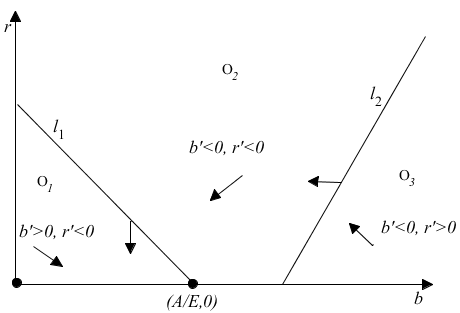
\includegraphics[scale=0.8]{Images/LoVae.png}
    \caption{Nullkliner \citep[s. 259]{Svensk}}
    \label{nulllovae}
\end{figure}

 Det ses, at nulklinerne deler det indre af 1. kvadrant op i 3 områder:
\begin{align*}
    O_1 &= \left\{(b,r) \in \mathbb{R}_+^2 \mid b \leq \frac{A}{E} , \ r \leq \frac{A}{B} - \frac{Eb}{B} \right\},\\
    O_2 &= \left\{(b,r) \in \mathbb{R}_+^2 \mid \frac{A}{E} - \frac{Br}{E} < b < \frac{C}{D} + \frac{Fr}{D} \right\},\\
    O_3 &= \left\{(b,r) \in \mathbb{R}_+^2 \mid b \geq \frac{C}{D} , \ r \leq -\frac{C}{F} + \frac{Db}{F}\right\}.
\end{align*}
Løsningskurverne igennem punkterne på $l_1$ vil have en tangent parallel med $r$-aksen, mens løsningskurverne igennem punkterne på $l_2$ vil have en tangent parallel med $b$-aksen.\\
I hvert af de tre områder, er $b'(t)$ og $r'(t)$ enten negativ eller positiv, som vist i figur \ref{nulllovae}. Vektorfeltets retning i hvert af de tre områder kan bestemmes på følgende måde. Vi indsætter konstanter i systemet \ref{lovaeIVP}, så uligheden $EC>AD$ er opfyldt. For eksempel:
\begin{equation*}
\begin{aligned}
    b'(t) &=\frac{1}{2}b(t)-\frac{1}{4}r(t)b(t)-\frac{1}{2}b(t)^2\\
    r'(t) &=\frac{1}{4}b(t)r(t)-\frac{1}{2}r(t)-\frac{1}{2}r(t)^2
\end{aligned}   
\end{equation*}
For at undersøge vektorfeltets retning i $O_1$ finder vi $b'(t)$ og $r'(t)$ i et punkt, som ligger i dette område. Dette punkt kunne for eksempel være $(1/4,1/4)$, og vi får: $b'(t)=\frac{5}{64}$ og $r'(t)=-\frac{9}{64}$. På samme måde findes vektorfeltets retning i de andre områder.\\ 
\hfill \break
De følgende argumenter er taget fra \citep[s. 258-259]{Svensk}. Lad os nu betragte løsningskurvernes opførsel i område $O_1$. På $l_1$ er $b'(t)=0$ og $r'(t)<0$, løsningskurverne vil derfor bevæge sig ind i det indre af $O_1$, hvor $b'(t)>0$ og $r'(t)<0$, og $b(t)$ er dermed en strengt voksende funktion, mens $r(t)$ er en strengt aftagende funktion i det indre af $O_1$. Da $b(t) \leq \frac{A}{E}$ er $b(t)$ altså opadtil begrænset i $O_1$ hvilket medfører, at der eksisterer et $\tilde{b} \geq 0$, så $\lim_{t \to \infty}b(t)=\tilde{b}$. I $O_1$ er $r(t)> 0$ og dermed nedadtil begrænset, hvilket medfører at der eksisterer et $\tilde{r} \geq 0$, så $\lim_{t \to \infty} r(t) = \tilde{r}$. 
\\  Løsningskurverne konvergerer altså mod et punkt, $(\tilde{b},\tilde{r})$, som må være et ligevægtspunkt for systemet ifølge følgende lemma:\\
\begin{lemma}{Grænseværdi for løsning \citep[s. 253]{Svensk}}{}
Lad $\vec{y}(t)$ være en løsning til et IVP, og lad IVP'ets maksimale definitionsinterval være $]a_1,\infty[$. Lad $\vec{y}(t)\to \hat{y}\in A$ for $t\to \infty$, hvor $A$ er defineret som i definition \ref{LoesningODE}. Så er $\hat{y}$ et ligevægtspunkt.
\end{lemma}
\begin{proof}\\
Lad $y_j(t)$ være den $j'$te koordinat i $\vec{y}(t)$. Da $\vec{y}(t)$ er en løsning, er $y_j(t)$ differentiabel på det åbne interval, $]t,t+1[ \ \subseteq \ ]a_1,\infty[$. Så følger det af middelværdisætningen, at
$$y_j(t+1)-y_j(t)= y_j'(\tau)=f_j(y_1(\tau),y_2(\tau),\hdots,y_n(\tau)),$$
 for et $\tau\in \ ]t,t+1[$, hvor $f_j$ er defineret som i definition \ref{autonom}. Når $t\to \infty$, går venstresiden mod $\hat{y}_j-\hat{y}_j=0$, og højresiden går mod $f_j(\hat{y})$. Dermed har vi, at $f_j(\hat{y})=0$ for alle $j$, og derfor er $\vec{f}(\hat{y})=0.$
\end{proof}\\ 
\hfill \break
Løsningskurverne i $O_1$ konvergerer altså mod et ligevægtspunkt.
Da $b(t)$ er strengt voksende i $O_1$, kan løsningskurverne ikke konvergere mod $(0,0)$, og den eneste mulighed er derfor $(\frac{A}{E},0)$.\\ 
\hfill \break
Vi betragter nu løsningskurverne med begyndelsespunkt i $O_2$. Det ses at $b'(t)< 0$ og $r'(t)<0$ i $O_2$, og både $b(t)$ og $r(t)$ er dermed aftagende funktioner. Grundet vektorfeltets retning kan en løsningskurve ikke bevæge sig ind i $O_3$, og den kan heller ikke skære akserne grundet EESFS. En løsningskurve, der forlader $O_2$, vil derfor gå ind i $O_1$, hvor vi ved, at den vil konvergere mod $(\frac{A}{E},0)$ for $t \to \infty$. Hvis løsningskurven forbliver i området $O_2$, ved vi, at $b(t)$ og $r(t)$ er aftagende og begrænsede funktioner. De har derfor en grænseværdi, og vi kan dermed anvende samme argumentation som før, for at vise at løsningskurverne konvergerer mod $(\frac{A}{E},0)$. \\ 
\hfill \break 
Til sidst betragtes løsningskurverne med begyndelsespunkt i $O_3$. På $l_2$ er $r'(t)=0$ og $b'(t)<0$. Derfor vil løsningskurverne bevæge sig ind i $O_2$. I det indre af $O_3$ er $r'(t)>0$ og $b'(t)<0$. Lad $(b_0,r_0)$ være et indre punkt i $O_3$ og lad $\Omega = \{(b,r) \in \mathbb{R}_+^2 | \frac{C}{D} \leq b \leq b_0, r \leq \frac{C}{F}+ \frac{Db}{F} \} $. Da $\Omega$ er en kompakt mængde, og $b'(t)$ er kontinuert, antager $b'(t)$ supremum på $\Omega$.
Sæt $S=\sup_{\Omega} b'(t)$, så er $b(t) \leq b_0 +tS$ i $\Omega$. Vi antager nu, at $b(t) \in \Omega  \ \forall t$. Da er $b(t) \geq \frac{C}{D}$. Men $\lim_{t \to \infty} b_0+tS= -\infty$, da $S<0$, hvilket medfører at $\lim_{t \to \infty} b(t)= -\infty$. Dette er en modstrid. Dermed eksisterer der et $t$, så $b(t)\leq \frac{C}{D}$. En løsningskurve, der starter i $O_3$, vil altså på et eller andet tidspunkt bevæge sig ind i $O_2$. Alle løsningskurver med et begyndelsespunkt i det indre af 1. kvadrant vil dermed konvergere mod $(\frac{A}{E},0)$.\\ 
\hfill \break 
I det ovenstående antog vi, at $a_2=\infty$ i det maksimale definitionsinterval $]a_1,a_2[$. Dette vil vi nu vise. Betragt nemlig figur \ref{nulllovae}. Det er klart, at $(b(t),r(t))\in [0,b_{max}]\times[0,y_{max}]$, som er en lukket og begrænset mængde. Antag nu, at $a_2\neq\infty$. Så er $(t,(b(t),r(t)))\in [0,a_2]\times[0,b_{max}]\times[0,y_{max}]$, som er en lukket og begrænset, og dermed kompakt, mængde. Derfor forlader den maksimale løsning denne mængde ifølge sætning \ref{forladkompakt}. Da $(b(t),r(t))\in [0,b_{max}]\times[0,y_{max}]$ for alle $t$, er den eneste mulighed, at $t$ forlader $[0,a_2]$. Det er en modstrid, og vi har altså at $a_2=\infty$. Det samme argument kan bruges for tilfældet, hvor $CE<AD$.
\\ \hfill \break
Vi antager nu, at $EC<AD$ i dette tilfælde vil ligevægtspunktet $(b_4^*,r_4^*)= \left(\frac{AF+BC}{EF+BD},\frac{AD-EC}{EF+BD}\right)$ ligge i 1. kvadrant. \\ \hfill \break
Som i tilfældet ovenfor kan vi bestemme vektorfeltets retning i de 4 områder; $O_1,O_2,O_3,O_4$, som er illustreret i figur (\ref{nulllovae2}).

\begin{figure} [H]
    \centering
    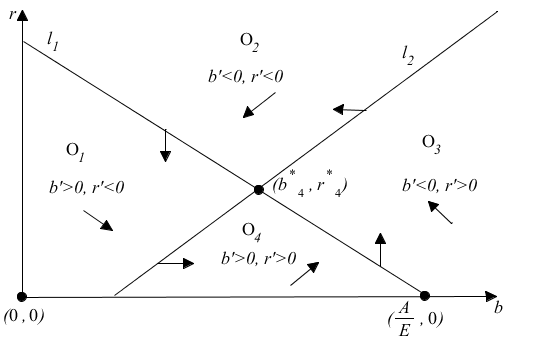
\includegraphics[scale=0.8]{Images/LoVae2.png}
    \caption{$(b_4^*,r_4^*)$ i 1. kvadrant.}
    \label{nulllovae2}
\end{figure}

Ved brug af de samme argumenter som i forrige tilfælde kan det vises at ligevægtspunktet $(b_4^*,r_4^*)$ er asymptotisk stabilt. \\ 
\hfill \break
Lad os først betragte løsningskurverne med begyndelsespunkt i $O_1$ og på $l_1$ for $r>r_4^*$. Hvis en sådan løsningskurve forlader området, $O_1$, vil den gå ind i $O_4$ på grund af vektorfeltets retning. Hvis den bliver i $O_1$, vil den konvergere mod $(b_4^*,r_4^*)$ med samme argument som før. Situationen er den samme i de andre områder. Enten konvergerer de mod $(b_4^*,r_4^*)$, eller de går ind i det næste område, jævnfør figur \ref{nulllovae2}. Dermed vil løsningskurverne med tiden bevæge sig ind mod ligevægtspunktet. Derfor er $(b_4^*,r_4^*)$ et asymptotisk stabilt ligevægtspunkt. 
\hfill \break

\section{Stabilitet af ligevægtspunkter i Lotka-Volterra med logistisk vækst}
Vi vender nu tilbage til systemets ligevægtspunkter og vil forsøge at beskrive dem ved hjælp af egenværdier.
Betragt Jacobi-matricen:
        \begin{equation}\label{jacobilovae}
        \textbf{J} =
        \frac{\partial\vec{f}}{\partial \vec{y}}=
         \begin{bmatrix}
        \frac{\partial j}{\partial b} & \frac{\partial j}{\partial r}\vspace{1mm}\\
        \frac{\partial l}{\partial b} & \frac{\partial l}{\partial r}
        \end{bmatrix}
        =
        \begin{bmatrix}
        A-Br-2Eb & -Bb\\
        Dr & Db-C-2Fr
        \end{bmatrix}
        \end{equation}
Hvis vi ser på ligevægtspunktet $(0,0)$ og indsætter dette i jacobi-matricen, fås:

        \[
        \textbf{J}_{\left(b^*_1,r^*_1 \right)} =
        \textbf{J}_{\left(0,0 \right)} =
        \begin{bmatrix}
        A & 0\\
        0 & -C
        \end{bmatrix}
        \]
Da er tilfældet det samme som for systemet uden logistisk vækst, og ligevægtspunktet er således et saddelpunkt. 
\hfill \break

Betragt nu Jacobi-matricen for $(b^*_2,r^*_2)$:
\begin{equation*}
    \textbf{J}_{\left(b^*_2,r^*_2 \right)} =
    \textbf{J}_{\left(0,-\frac{C}{F}\right)} =
        \begin{bmatrix}
        A + \frac{BC}{F} &  0\\
        -\frac{CD}{F} & C
        \end{bmatrix}
\end{equation*}
Vi indsætter denne matrix i vores ligning for at finde egenværdier:

$$
    \left(\textbf{J}_{\left(0,-\frac{C}{F}\right)}-\lambda I\right) =
        \begin{bmatrix}
        A + \frac{BC}{F} &  0\\
        -\frac{CD}{F} & C
        \end{bmatrix}-
    \begin{bmatrix}
    \lambda & 0\\
    0 & \lambda
    \end{bmatrix} =
        \begin{bmatrix}
        A + \frac{BC}{F} - \lambda &  0\\
        -\frac{CD}{F} & C - \lambda
        \end{bmatrix}
$$
Da findes $\det(\textbf{J}-\lambda I)$:

$$\left( A + \frac{BC}{F} - \lambda\right)(C - \lambda) = 0$$
Da er det klart, at egenværdierne for ligevægtspunktet $(0, -\frac{C}{F})$ er reelle og forskellige med samme fortegn, hvoraf det kan konkluderes, at ligevægtspunktet er en kilde og løsningskurverne vil bevæge sig væk fra ligevægtspunktet, hvorfor det er et ustabilt ligevægtspunkt, jævnfør \ref{tab:egenvardi}.
\hfill \break

Betragt nu Jacobi-matricen for $(b^*_3,r^*_3)$:
\begin{equation*}    
   \textbf{J}_{\left(b^*_3,r^*_3 \right)} =
    \textbf{J}_{\left(\frac{A}{E},0\right)} =
        \begin{bmatrix}
        -A &  \frac{AB}{E}\\
        0 & \frac{AD}{E}-C
        \end{bmatrix}
\end{equation*}
Vi indsætter denne matrix i vores ligning for at finde egenværdier:

$$
    \left(\textbf{J}_{\left(\frac{A}{E},0\right)}-\lambda I\right) =
        \begin{bmatrix}
        -A &  \frac{AB}{E}\\
        0 & \frac{AD}{E}-C
        \end{bmatrix}-
    \begin{bmatrix}
    \lambda & 0\\
    0 & \lambda
    \end{bmatrix} =
        \begin{bmatrix}
        -A - \lambda &  \frac{AB}{E}\\
        0 & \frac{AD}{E}-C-\lambda
        \end{bmatrix}
$$
Da findes $\det(\textbf{J}-\lambda I)$:

$$(-A - \lambda)\left(\frac{AD}{E}-C-\lambda\right) = 0$$

Egenværdierne er
\begin{align*}
    \lambda_1&=-A \\
    \lambda_2&=\frac{AD}{E}-C
\end{align*}

Det er nu klart, at egenværdierne for ligevægtspunktet $\left( \frac{A}{E} , 0 \right)$ er reelle. Egenværdierne for ligevægtspunktet vil enten være forskellige og med samme fortegn, eller forskellige med forskelligt fortegn alt efter hvilket led i $\lambda_2$, der er størst. 
I tilfældet, hvor $\frac{AD}{E} > C$, vil $\lambda_2 > 0$, og dermed er ligevægtspunktet et saddelpunkt og ustabilt. I tilfældet, hvor $\frac{AD}{E} < C$, vil $\lambda_2 < 0$, og dermed er ligevægtspunktet et dræn, hvormed løsningskurverne vil bevæge sig imod ligevægtspunktet, hvorfor det er asymptotisk stabilt, jævnfør tabel \ref{tab:egenvardi}. Dette stemmer overens med analysen i afsnit \ref{lovaelovo}. \hfill \break

%Jacobi-matricen for $(b^*_4,r^*_4)$ er en meget kompliceret beregning og vil derfor ikke blive undersøgt.% For simpelhedens skyld undersøges derfor tilfældet, hvor $F=0$. Derved er Jacobi-matricen:
% \begin{equation*}
%        \textbf{J} =
%        \begin{bmatrix}
%        A-Br-2Eb & -Bb\\
%        Dr & Db-C
%        \end{bmatrix}
%        \end{equation*}
%Ligevægtspunktet vil også ændres til $(b^*_4,r^*_4)=(\frac{BC}{BD}, \frac{AD-EC}{BD})$. Ved indsættelse i Jacobi-matricen fås derved:
%\begin{equation*}
%    \textbf{J}_{\left(b^*_4,r^*_4 \right)} =
%     \begin{bmatrix}
%        A-B\frac{AD-EC}{BD}-2E\frac{BC}{BD} &  -B\frac{BC}{BD}\\
%        D\frac{AD-EC}{BD} & D\frac{BC}{BD}-C
%        \end{bmatrix}
%    =\begin{bmatrix}
%        -\frac{EC}{D} & -\frac{BC}{D}\\
%        \frac{AD-CE}{B} & 0
%        \end{bmatrix}
%\end{equation*}
%Det karakteristiske polynomium til denne matrix er derved
%\begin{equation*}
%    \det(\textbf{J}_{\left(b^*_4,r^*_4 \right)}-\lambda I_4)= \lambda^2+\lambda\frac{EC}{D}+\frac{C(AD-CE)}{D}=0
%\end{equation*}
%   
%Diskriminanten dertil er
%\begin{align*}
%    &d=\left(\frac{EC}{D}\right)^2-4\left(AC-\frac{CE^2)}{D} \right)
%\end{align*}
% \hfill \break
%og egenværdierne er
%\begin{align*}
%   \lambda&=-\frac{EC}{2D} \pm \frac{1}{2}\sqrt{\left(\frac{EC}{D}\right)^2-4\left(AC-\frac{CE^2}{D} \right)}\\
%   &= -\frac{EC}{2D} \pm \sqrt{\left(\frac{EC}{2D}\right)^2-\left(AC-\frac{CE^2}{D} \right) } \\
%   &= -\frac{EC}{2D} \pm \sqrt{\left(\frac{EC}{2D}\right)^2-AC\cdot\left(\frac{EC}{D}\right)^2\cdot\frac{4D^2}{E^2C^2}-\frac{CE^2}{D}\cdot\left(\frac{EC}{D}\right)^2\cdot\frac{4D^2}{E^2C^2}}\\
%   &=\left(\frac{EC}{2D}\right)^2 \left(-1\pm \sqrt{1+\frac{4D}{E}-\frac{4AD^2}{E^2C}}\right)
%\end{align*}

%Dermed kan det fastslås, at egenværdierne er komplekst konjugerede værdier med negativ realdel, hvis
%\begin{align}
%    E<4D\left(\frac{AD}{EC}-1\right),
%\end{align}
%og dermed må ligevægtspunktet $(b^*_4,r^*_4)$ være asymptotisk stabilt for disse $E$, og løsningskurven vil bevæge sig i en spiral ind mod dette punkt.
%\hfill \break
%Dermed må det være muligt at finde en streng Lyapunov funktion i ligevægtspunktet.
%\hfill \break 

I det følgende antages det, at uligheden $AD > EC$ er opfyldt, og Jacobi-matricen for $(b^*_4,r^*_4)$ betragtes.
Først indser vi, at $(b^*_4,r^*_4)$ er et ligevægtspunkt, hvor $j$-nulklinen og $l$-nulklinen krydser. Da ligevægtspunktet ligger i det indre af 1. kvadrant, må der gælde, at $r > 0$ og $b > 0$, hvoraf $j$- og $l$-nulklinerne, pér \eqref{nulkliner1}, er givet ved:
\begin{align*}
    A - Br - Eb &=0\\
    Db -C -Fr &=0
\end{align*}
Da fås, jævnfør ligning \eqref{jacobilovae}:
 \begin{equation*}
    \textbf{J}_{(b_4^*, r_4^*)} = \textbf{J}_{(\frac{AF+BC}{EF+BD}, \frac{AD-EC}{EF+BD})} = \begin{bmatrix}
    -E\left( \frac{AF+BC}{EF+BD}\right) & -B\left( \frac{AF+BC}{EF+BD} \right) \\
    D \left(\frac{AD-EC}{EF+BD} \right) & -F \left( \frac{AD-EC}{EF+BD}\right)
        \end{bmatrix}.
\end{equation*}


For overskuelighedens skyld benyttes $(b_4^*,r_4^*)$ indledningsvist i det følgende. Først findes $\det(\textbf{J}_{(b_4^*,r_4^*)}-\lambda I)$:
\begin{align*}
   \det(\textbf{J}_{(b_4^*,r_4^*)}-\lambda I) &= \left( -Eb_4^* -\lambda \right) \left( -F r_4^*-\lambda\right)+ Dr_4^*Bb_4^* \\
   &=\lambda^2 + (Eb_4^* + F r_4^*)\lambda + (EF(b_4^*r_4^*) + DB(b_4^*r_4^*))
\end{align*}
Fra dette udledes, at $4(EF(b_4^*r_4^*) + DB(b_4^*r_4^*)) > ((Eb_4^* + F r_4^*)\lambda)^2$, hvis der skal eksistere komplekse rødder for den karakteristiske ligning, som også kan skrives som,
$$((ADF+AEF+BCE-CEF)\lambda)^2 < 4(A^2DF+ABCD-ACEF-BC^2E)$$






%\begin{align*}
%   \det(\textbf{J}_{(b_4^*,r_4^*)}-\lambda I) &= \left( -E\left( \frac{AF+BC}{EF+BD}\right)-\lambda \right) \left( -F \left( \frac{AD-EC}{EF+BD}\right)-\lambda\right)+ \frac{D(AD-CE)B(AF+BC)}{(BD+EF)^2} \\
%   &=\lambda^2 + \frac{(ADF+AEF+BCE-CEF)\lambda}{BD+EF}+\frac{A^2DF+ABCD-ACEF-BC^2E}{BD+EF}.
%\end{align*}
\textbf{Vi har ikke vist at rødderne til det karakteristiske polynomium er komplekse. I det følgende antager vi imidlertid, at det gælder.}
I den videre bearbejdelse af ligevægtspunktet, $\textbf{J}_{(b^*_4, r^*_4)}$, antages det, at det karakteristiske polynomium, som beskrevet ovenfor, har komplekse rødder. Der indføres nu følgende lemma, for at gøre analysen af egenværdier for $\textbf{J}_{(b^*_4, r^*_4)}$ mulig:
\begin{lemma}{Den komplekskonjugerede rodsætning}{egvdjacobi}
Hvis $\lambda^2 + a \lambda +b=0$, hvor $a, b \in \mathbb{R}$ har en kompleks rod, $\lambda_0$, så er $\bar{\lambda}_0$ også en rod.
\end{lemma}

\begin{proof}\\
Lad $\lambda_0 \in \mathbb{C}$ være en rod til $\lambda^2 +a \lambda +b = 0$, hvor $a, b \in \mathbb{R}$. Da fås ud fra $\lambda_0^2 +a \lambda_0 +b = 0$, at
$$(\bar{\lambda_0})^2 +a \bar{\lambda}_0 +b = \bar{0}=0,$$
hvormed $\bar{\lambda}_0$ også er en rod.
\end{proof}
\\ \hfill \break
\textbf{Bemærk:} Lemma \ref{th:egvdjacobi} fortæller, at når $\lambda_0 = \alpha + i \beta$ fås, så gælder følgende
\begin{align*}
    \lambda^2 +a\lambda +b &= (\lambda-(\alpha +i \beta))(\lambda - (\alpha - i \beta)) \\
    &= (\lambda - \alpha)^2 -(i \beta)^2 \\
    &= \lambda^2-2 \alpha \lambda + \alpha^2 + \beta^2.
\end{align*}
Hvormed
\begin{equation*}
\begin{cases}
    a &= -2 \alpha, \\
    b &= \alpha^2 + \beta^2.
\end{cases}
\end{equation*}
Dermed er det nok at kende fortegnet på $a$, for at bestemme fortegnet på realdelen af roden.\\ \hfill \break
Det ønskes kun at undersøge egenværdierne for ligevægtspunktet, når det eksisterer i det indre af 1. kvadrant, da løsningskurverne, i det tilfælde hvor ligevægtspunktet er i 4. kvadrant, vil ende i ligevægtspunktet $(b^*_3, r^*_3)$. Ligevægtpunktet, $(b^*_4, r^*_4)$, ligger i det indre af 1. kvadrant, når uligheden, $AD > CE$, er opfyldt. Ved brug af denne ulighed ses det, at
$$\frac{(ADF+AEF+BCE-CEF)}{BD+EF} > 0,$$
og dermed vil egenværdierne $\lambda_0$ og $\bar{\lambda}_0$ for
$\textbf{J}_{(b^*_4, r^*_4)}$ have negativ realdel. Derfor er ligevægtspunktet, $(b^*_4, r^*_4)$, et spiralpunkt.
\hfill \break

En anden metode der kan benyttes er en Lyapunov funktion. Følgende proposition undersøges. 
\begin{prop}{Eksistens af streng Lyapunov funktion i logistisk vækst af Lotka-volterra's model}{elovae}
$E_f(u, v) = \left( u-b^* \ln{\left( \frac{u+b^*}{b^*} \right)} \right) + \frac{B}{D} \left( v-r^* \ln{\left( \frac{v+r^*}{r^*} \right)} \right)$, hvor $u=b-b^*, v=r-r^*$, er en streng Lyapunov funktion til systemet \eqref{lovaeIVP}.
\end{prop}

\begin{proof}
Det efterprøves om Lyapunov funktionen er lig 0, ved ligevægtspunktet $(b_4^*,r_4^*)$
$$E(b^*, r^*) =  \left( 0-b^* \ln{(1)} \right) + \frac{B}{D} \left( 0-r^* \ln{(1)} \right)=0.$$
 
Det ses at, når $u=0=v$ er der tale om et ekstremumspunkt, da $\frac{\partial E}{\partial u}(0,0)=0$ og $\frac{\partial E}{\partial v} (0,0)=0$. Hesse matricen undersøges nu for $E$:. 
 \begin{align*}
     H&=\begin{bmatrix}
     \frac{ b^*}{(u+b^*)^2} & 0 \\
     0 & \frac{\frac{B}{D}\cdot r^*}{(v+r^*)^2}
     \end{bmatrix}\\
     \det (H)&= \frac{ b^*}{(u+b^*)^2} \cdot \frac{\frac{B}{D} r^*}{(v+r^*)^2} > 0 \ \text{for} \ b,r>0\\
     \textnormal{trace}(H)&= \frac{ b^*}{(u+b^*)^2} + \frac{\frac{B}{D} r^*}{(v+r^*)^2} > 0 \ \text{for} \ b,r>0\\
 \end{align*}
 
 Jævnfør sætning \ref{th:Hesse}, ligning \eqref{det10} og \eqref{trace} er punktet dermed lokalt minimum for $E$, og $E(u,v) > 0$ for $u \neq 0, v \neq 0$.
 \hfill \break
Det undersøges nu, om $E$ er streng Lyapunov funktion, $\dot{E}_f < 0$:
$$\dot{E}_f (b, r)=\frac{\partial E}{\partial u}j(b,r) + \frac{\partial E}{\partial v}l(b,r) =  \left( 1 - \frac{b^*}{u+b^*}\right) b (A-Eb-Br) + \frac{B}{D} \left( 1 - \frac{r^*}{v+r^*}\right) r (Db-Fr-C),$$
hvis $AD > EC \Rightarrow b^*, r^* > 0$, så er de skrå nulkliner
$$A-Eb^*-Br^* = 0$$
$$Db^*-Fr^*-C = 0.$$

Vi kan nu subtrahere 0 fra udtrykket: 
\begin{align*}
    A-Eb-Br &= A-Eb-Br-(A-Eb^*-Br^*) \\
    &=-E(b-b^*)-B(r-r^*) \\
    &=-Eu-Bv,
\end{align*}
og
\begin{align*}
    Db-Fr-C &= Db-Fr-C-(Db^*-Fr^*-C) \\
    &=D(b-b^*)-F(r-r^*) \\
    &=Du-Fv.
\end{align*}

Derfor
\begin{align*}
    \dot{E}_f(u, v) &= \left( u + b^* - \frac{b^*(u+b^*)}{u+b^*} (-Eu-Bv) \right) + \frac{B}{D} \left( v + r^* - \frac{r^*(v+r^*)}{v+r^*} (Du-Fv) \right) \\
    &= u(-Eu-Bv) + \frac{B}{D} v(Du-Fv) \\
    &= (-Eu^2-Bvu) + \frac{B}{D} (Duv-Fv^2) \\
    &= - Eu^2- \frac{B}{D}  Fv^2 -(\frac{B}{D} - B)uv
\end{align*}
Dette kan også skrives på matrix form:
\begin{align*} 
&= \dot{E}_f(u,v). \\
&= -  Eu^2- \frac{BFv^2}{D}-(\frac{B}{D} - B)uv \\
&= - \frac{1}{2} (2E u^2 + \frac{FB}{D} v^2 + 2 uv(B - \frac{B^2}{D})) \\
&= - \frac{1}{2} \begin{bmatrix}
2E u + v(B + B) & \frac{2EB}{D} v 
\end{bmatrix}
\begin{bmatrix}
u \\
v
\end{bmatrix}\\
&= - \frac{1}{2} \begin{bmatrix}
u & v
\end{bmatrix} 
\begin{bmatrix}
2E & 0 \\
0 & \frac{2FB}{D}
\end{bmatrix}
\begin{bmatrix}
u \\
v
\end{bmatrix} 
\end{align*}

Vi betegner nu $S:= \begin{bmatrix}
2E & 0\\
0 & \frac{2FB}{D}
\end{bmatrix}$. Vi ønsker nu at undersøge om $\vec{l}^T S \vec{l} > 0$. Altså undersøges om $S$ er positivt definit for en given vektor $\vec{l} \neq 0$.
Matricen $S$ er symmetrisk. For at være positivt definit skal egenværdierne for $S$ være positive. Dette betyder at determinanten og sporet skal være positive. 
Altså $$\det (S) > 0 \ \textnormal{og} \ \textnormal{trace} (S) > 0,$$ hvor $\textnormal{trace}(S)=\lambda_1 + \lambda_2$ og $\det(S)=\lambda_1\lambda_2$. Dermed: 
\begin{align*}
    \textnormal{trace(S)} &=2E + \frac{2FB}{D}> 0\\
    \det(S) &=\frac{4EFB}{D} >0 \\
\end{align*}

Dermed er $E(b,r)$ streng Lyapunov funktion i første kvadrant.

\end{proof}\\ \hfill \break
\chapter{Diskussion}
I det følgende vil de to modeller af rovdyr-byttedyr systemet, som præsenteret i rapporten, blive diskuteret.\\
\hfill \break
Indledningsvis ville Lotka-Volterra's rovdyr-byttedyr system undersøges uden nogen modifikation til dette. Jævnfør de 6 antagelser fra indledningen, så vil dette system afbillede en interaktion mellem byttedyr og rovdyr i et isoleret system, og det er imidlertid ikke realistisk at sådan et system eksisterer i virkeligheden. Derfor inkluderes en modifikation til systemet, hvor en kapacitetsbegrænsing indføres for både byttedyr og rovdyr. Således vil byttedyrene ikke have ubegrænset føde, hvormed man er et skridt tættere på at kunne afbillede en virkelig situation. \\
\hfill \break
I dette projekt betragtes tilfældet, hvor systemet er modificeret med logistisk vækst, når både rovdyr og byttedyr har en kapacitetsbegrænsing
Afhængigt af værdierne af konstanterne i systemet viser stabilitetsanalysen, at de to populationer vil konvergere imod et ligevægtspunkt $(b_3^*,r_3^*)$ ,  eller et ligevægtspunkt $(b_4^*,r_4^*)$ i 1. kvadrant.\\
\hfill \break
Den signifikante forskel på de to førnævnte ligevægtspunkter, består i, at for ligevægtspunktet $(b_3^*, r_3*)$, vil rovdyrene uddø over tid uafhængigt af startpopulationen, såfremt punktet ligger på den positive b-akse. Dermed er det vigtigt, at konstanterne i systemet er nøje valgt med udgangspunkt i de to populationer af byttedyr og rovdyr, man ønsker at undersøge. Der forekommer altså markante ændringer i forhold til det ikke-modificerede system, når man begrænser de to populationer. Ligevægtspunktet går fra stabilt i det ikke-modificerede til asymptotisk stabilt, hvor rovdyrene vil uddø.\\
\hfill \break
Sammenlignes den ikke-modificerede og den modificerede model i henhold til ligevægtspunktet $(b_4^*,r_4^*)$ i 1. kvadrant, ses der også en klar forskel. I dette tilfælde vil den modificerede model, hvor begge populationer er begrænsede, have et asymptotisk ligevægtspunkt. Dette betyder, at begge populationer vil konvergere imod ligevægtspunktet, når $t \to \infty$. De to populationerne vil således ikke indgå i en uendelig cyklus, hvor størrelsen af de to populationer konstant varierer, men vil derimod nå et punkt, hvor de to arters populationer er konstant, og ikke længere påvirkes af hinanden. De to populationer er altså i ligevægt. \\
\hfill \break
%Betragtes situationen, hvor det udelukkende er byttedyrene, der er begrænset i det modificerede system, så vil $f=0$. Det bemærkes, at dette system er et specialtilfælde af systemet i \eqref{lovaeIVP}, hvorfor systemet indebærer denne begrænsning af rovdyrene, så der ikke udelukkende ses på et specialtilfælde.
\chapter{Konklusion}
Denne rapport vil afslutningsvist indeholde en konklusion af problemformuleringen, som lyder:\\
\hfill \break
Hvordan bruges et system af differentialligninger til at modellere et byttedyr-rovdyr system, og hvilken indflydelse har det på systemet, hvis væksten af henholdsvis byttedyrene og rovdyrene er begrænset?\\
\hfill \break
Det er klart, at et system af differentialligninger er anvendeligt i den situation, hvor man står med en ligning, der er afhængig af løsningen til en anden ligning. Det vil sige, at differentialligningssystemer er anvendelige, når man har to ubekendte funktionsværdier, som er indbyrdes afhængige. Et problem af en sådan udformning, gør det imidlertid besværligt, at finde en eksakt løsning, men det giver mulighed for en kvalitativ analyse med udgangspunkt i det opstillede system.\\
\hfill \break
I det modificerede system ses der en klar forskel fra det ikke-modificerede system. Den markante ændring, som følge af modifikationen, er, at der forekommer asymptotiske ligevægtspunkter, hvormed de to populationer vil konvergere imod disse, når $t \to \infty$. Dermed vil det modificerede system opnå ligevægt over tid, hvorimod det ikke-modificerede aldrig vil opnå ligevægt og består i en uendelig cyklus.\\
\hfill \break
Konklusionen er dermed, at en kapacitetsbegrænsning på en eller begge af populationerne vil indebære, at populationerne opnår ligevægt over tid.
%\chapter{Ekstra-stuff}

\subsection{Mikkel}

\subsection{Lipschitz-kontinuitet}
Lipcshitz-kontinuitet er første skridt i at bevise eksistens- og entydighedssætningen for løsninger til differentialligninger?
\begin{definition}[Lipschitz-kontinuitet]
Givet en funktion, $f: (t,\vec{x})\in R \subseteq \mathbb{R}^{m+1} \rightarrow f(t,\vec{x}) \in \mathbb{R}^m$, kaldes Lipschitz-kontinuert, hvis $\exists L \geq 0$, så:
$$|f(t,\vec{x_1})-f(t,\vec{x_2})|\leq L|\vec{x_1}-\vec{x_2}|$$
\end{definition}

\begin{Example}\textbf{Lipschitz-kontinuitet}\hfill \break
\textnormal{Hvis vi lader $\mathbb{R}^2$ være det réelle plan og betragter funktionen $f(t,x)=t^5+4x$, så kan vi undersøge om $f$ er Lipschitz-kontinuert på $\mathbb{R}^2$:} \hfill \break
$$|f(t,x_1)-f(t,x_2)|=|(t^5+4x_1)-(t^5+4x_2)|=|4x_1-4x_2|=4|x_1-x_2|$$ \hfill \break
\textnormal{Det ses nu, at funktionen opfylder en Lipschitz betingelse på $\mathbb{R}^2$ med $L=4$.}
\end{Example}
\begin{lemma}{}{}
Lad $D$ være et lukket rektangel $R=(a,b)\times(c,d)$ eller en uendelig strimmel $S=(a,b)\times(-\infty,\infty)$ på planet $\mathbb{R}^2$. $f$ er Lipschitz-kontinuert på $R$ eller $S$ hvis:

\begin{enumerate}
    \item $f:D \rightarrow \mathbb{R}$
    \item $\frac{\partial f}{\partial y}$ eksisterer og er kontinuert
    \item Der eksisterer en konstant $K\geq 0$ sådan, at $|\frac{\partial f}{\partial y}(t,y)|\leq K$
\end{enumerate}

Dermed er $K=L$
\end{lemma}
\begin{proof} \hfill \break
Ved brug af fundamental calculus gælder, at for alle $(t,y_1),(t,y_2) \in D$ er
\begin{align}
 f(t,y_1)-f(t,y_2)=\int_{y_2}^{y_1}\frac{\partial f}{\partial y} dy \notag
\end{align}
og derved
\begin{align}
 |f(t,y_1)-f(t,y_2)|&=|\int_{y_2}^{y_1}\frac{\partial f}{\partial y} dy| \notag \\
&\leq |\int_{y_2}^{y_1}|\frac{\partial f}{\partial y}| dy| \notag\\
&\leq |\int_{y_2}^{y_1}K| \notag \\
&=K|y_1-y_2| \notag
\end{align}
hvilket giver $K=L$ ifølge definitionen af Lipschitz-kontinuitet. \qedhere
\end{proof}
\hfill \break

\begin{Example}\hfill \break
\textnormal{Betragt funktionen $f(t,y)=t^5+\tan^{-1}(y)$. Hvis vi benytter Lemma 2.3.1 får vi:} \hfill \break
\begin{align}
\frac{\partial f}{\partial y}=\frac{1}{1+y^2} \notag
\end{align}
\textnormal{Det ses hurtigt, at brøken $\frac{1}{1+y^2}$ altid vil være mindre end eller lig med 1 for alle $(t,y)\in \mathbb{R}^2$, altså:}
\begin{align}
 \frac{1}{1+y^2}\leq 1, \forall(t,y) \in \mathbb{R}^2 \notag
\end{align}
\textnormal{Dermed ses, at $L=1$, og $f$ er Lipschitz-kontinuert på $\mathbb{R}^2$.}
\end{Example}

\subsection{Banachs fixpunktssætning}

\begin{definition}[Metrisk rum]
Et metrisk rum er et ordnet par $(M,d)$, hvor $M$ er en mængde og $d$ er en metrik $d:M\times M \rightarrow \mathbb{R}_+$, $d(x,y)=|x-y|$, hvorom der gælder for ethvert $x,y,z \in M$: 
\begin{enumerate}
    \item $d(x,y)=0 \Leftrightarrow x=y$ 
    \item $d(x,y)=d(y,x)$
    \item $d(x,z)\leq d(x,y)+d(y,z)$
\end{enumerate}
$d$ kaldes også for afstandsfunktionen.
\end{definition}

\begin{definition}[Cauchyfølger i Metriske rum]
En talfølge $\{x_n\}$ i et metrisk rum $(M,d)$ siges at være Cauchyfølge, hvis der for enhver positiv tolerencegrad $\varepsilon >0$ eksisterer $N \in \mathbb{N}$, så der for alle $m,n \geq N$, $m,n \in \mathbb{N}$ gælder, at: 
$$|x_n-x_m|<\varepsilon$$
\end{definition}

\begin{definition}[Fuldstændigt metrisk rum]
Et metrisk rum $(M,d)$ siges at være fuldstændigt, hvis alle Cauchyfølger i $M$ har en grænse, der også er i $M$. Altså hvis alle Cauchyfølger i $M$ konvergerer i $M$.
\end{definition}

\begin{definition}[Kontraktion og Fixpunkt]
Lad $(M,d)$ være et metrisk rum. En afbildning $F:M\rightarrow M$ kaldes en kontraktion, hvis der eksisterer en Lipschitz-konstant $0 \leq L < 1$, sådan at:
$$|F(x_1)-F(x_2)|\leq L|x_1-x_2|$$
Et punkt $x \in M$ er et fixpunkt for $F$, hvis $F(x)=x$ 
\end{definition}

\begin{mytheo}{Banachs fixpunktssætning}
LLad $(X,d)$ være et fuldstændigt metrisk rum og $F:X\rightarrow X$ være en kontraktion. Så har $F$ et unikt fixpunkt.
\end{mytheo}

\begin{proof}
Først viser vi unikheden af fixpunktet. Antag at der eksisterer $a,b \in M$, så $F(a)=a$ og $F(b)=b$, så antyder Definition 2.12, at \hfill \break
$$0\leq d(a,b)=d(F(a),F(b))\leq Ld(a,b), (1-L)|y_1-y_2|\leq 0$$
hvilket betyder at $d(a,b)=0$ og at $a=b$ \hfill \break
\hfill \break
Vi konstruerer nu sådan et fixpunkt. Betragt talfølgen ${y_n}$, hvor $y_1$ er arbitrær og $y_n:=F(y_{n-1})$ for ethvert $n\geq 2$. Vi ønsker nu at vise to ting:\hfill \break
 ($i$) Talfølgen er Cauchyfølge i M og dermed konvergerer mod et $y_\infty$, da vi antog at $M$ var fuldstændigt metrisk rum.\hfill  \break
($ii$) $y_\infty$ er et fixpunkt for $F$. \hfill \break
Vi starter med ($i$). For enhver tolerancegrad $\epsilon > 0$ vil vi konstruere et $N > 0$ sådan at for alle $p\geq q \geq N$ har vi $d(y_q,y_p)<\epsilon$. Dette kan også skrives \hfill \break
\begin{align}
d(y_q,y_{q+k})<\epsilon,  \forall k \geq 0, \forall q \geq N
\end{align}
Hvis $k \geq 1$ antyder trekantsuligheden, at \hfill \break
\begin{align}
d(y_q,y_{q+k}) &\leq d(y_{q},y_{q+1})+d(y_{q+1},y_{q+k}) \notag\\
&\leq d(y_q,y_{q+1})+d(y_{q+1},y_{q+2})+d(y_{q+2},y_{q+k}) \notag\\
&\leq \sum\limits_{r=0}^{k-1} d(y_{q+r},y_{q+r+1})
\end{align}
For ethvert $n\geq 1$ har vi \hfill \break
$$d(y_n,y_{n+1})=d(F(y_{n-1}),F(y_n)) \leq Ld(y_{n-1},y_n) \leq \hdots \leq L^{n-1}d(y_1,y_2), \forall n \geq 1$$
Dermed er $d(y_{q+r},y_{q+r+1}) \leq L^{n-1}d(y_1,y_2)$ for alle $q \geq 1$ og $r\geq 0$. Dette og (2.4) giver, at \hfill \break
$$d(y_q,y_{q+k}) \leq L d(y_1,y_2)(1+\hdots+L^{k-1}) \leq \frac{L^{q-1}}{1-L}d(y_1,y_2), \forall k \geq 1$$
ved at bruge $(1-L)(1+L^2+\hdots+L^{k-1})=1+L^2+\hdots +L^{k-1}-L-L^2-\hdots -L^k= 1-L^k \leq 1$. \hfill \break
Da $0 \leq L < 1$ må $\lim_{q\rightarrow\infty} L^q=0$ og (2.3) må gælde. Det kan dermed konkluderes, at der eksisterer $y_\infty \in X$ sådan at \hfill \break
$$\lim_{n \to \infty} d(y_n,y_\infty)=0$$
Dermed må $\{y_n\}$ være Cauchyfølge i $M$. \hfill \break

Nu bevises ($ii$). For ethvert $n \geq 1$ gælder:
$$d(F(y_\infty),y_\infty)\leq d(F(y_\infty),F(y_n))+d(F(y_n),y_\infty)$$
Da $d(F(y_\infty),F(y_n))\rightarrow 0$ og $\lim_{n \to \infty} d(F(y_n),y_\infty) = \lim_{n \to \infty} d(y_{n+1},y_\infty)=0$, så må $d(F(y_\infty),y_\infty)=0$ og dermed $F(y_\infty)=y_\infty$. Så $y_\infty$ er unikt fixpunkt for $F$.
\end{proof}

\subsection{Bevis af Picard-Lindelöf sætningen}

\begin{definition}[Normeret vektorrum og Banachrum]
Hvis et vektorrum $V$ over et legeme $\mathbb{F}$ har normen af alle vektorer i $V$ defineret ved funktionen $||\cdot||:V\to \mathbb{R}_+$, kaldes det ordnede par $(V,||\cdot||)$ et normeret vektorrum.
Hvis alle Cauchyfølger af vektorer $\{\vec{v}_n\}$ i $V$ konvergerer mod en anden vektor $\vec{v}_\infty$ i $V$, kaldes det normerede vektorrum et fuldstændigt normeret vektorrum eller et Banachrum.
\end{definition}

\begin{proof}
Det var beviset.
\end{proof}

\subsection{Jacobi-matricer}

For at kunne beskrive ikke-lineære systemer omkring et ligevægtspunkt, indføres følgende

\begin{definition}[Jacobi-matrix]
Lad $$\textbf{f}: \mathbb{R}^n \to \mathbb{R}^m$$ være en funktion der afbilleder en vektor, $$\vec{x} \in \mathbb{R}^n$$ over i $$\textbf{f}(\vec{x}) \in \mathbb{R}^m \text{.}$$ \\ Da defineres en $m \times n$ matrix, $\textbf{J}$, på $\textbf{f}$ til at være den Jacobianske matrix til funktionen og skrives på formen:
$$\textbf{J}_f(\vec{x}) = \frac{d\textbf{f}}{d\vec{x}} =
\begin{bmatrix}
    \frac{\partial \textbf{f}_1}{\partial \vec{x_{1}}} & \frac{\partial \textbf{f}_1}{\partial \vec{x_{2}}} & \dots & \frac{\partial \textbf{f}_1}{\partial \vec{x_{n}}} \\
    \frac{\partial \textbf{f}_2}{\partial \vec{x_{1}}} & \frac{\partial \textbf{f}_2}{\partial \vec{x_{2}}} & \dots & \frac{\partial \textbf{f}_2}{\partial \vec{x_{n}}} \\
    \vdots & \vdots & \ddots & \vdots \\
    \frac{\partial \textbf{f}_m}{\partial \vec{x_{1}}} & \frac{\partial \textbf{f}_m}{\partial \vec{x_{2}}} & \dots & \frac{\partial \textbf{f}_m}{\partial \vec{x_{n}}}
\end{bmatrix},$$
eller komponentvist:
$$\textbf{J}_{ij} = \frac{\partial \textbf{f}_i}{\partial \vec{x}_j}$$

Den Jacobianske matrix er en lineær afbildning $\mathbb{R}^n \to \mathbb{R}^m$, der angiver en lineær approksimation af $\textbf{f}$ til et $\vec{x}$.
\end{definition}

\begin{definition}[]
Lad $\textbf{f}$ være en funktion og $a \in \mathbb{R}^n$ være et punkt. Er $\textbf{f}$ differentiabel i $a$, er dens afledte givet ved $\textbf{J}_f({a})$. I dette tilfælde siges den lineære afbildning givet den Jacobianske-matrix at være den bedste lineære approksimation af $\textbf{f}$ til $a$.

\hfill \break
Denne lineære approksimation skrives:

$$\textbf{f}(x)=\textbf{f}(a)+ \textbf{J}_f({a})(x-a)+ o(\left. \Vert \left. x-a \right. \Vert \right.),$$ 
for $x \to a$.

\end{definition}

\begin{definition}[Hyperbolsk ligevægtspunkt]
%asfAFASF
\end{definition}

\begin{Example}

$$\textbf{F(x)} =
\begin{bmatrix}
x_1 x_3^2 -e^{x_1 x_2} \\
x_2 - \frac{1}{x_3} \\
x_1 x_2 x_3
\end{bmatrix} \Rightarrow
J_{f}(x) =
\begin{bmatrix}
    x_3^2 - x_2 e^{x_1 x_2} & -x_1 e^{x_1 x_2} & 2x_1 x_3 \\
    0 & 1 & \frac{1}{x_3^2}\\
    x_2 x_3 & x_1 x_3 & x_1 x_2
\end{bmatrix}$$

\end{Example}



\chapter*{Grænseværdi}

\begin{definition}[Punktfølge]
En punktfølge består af uendeligt mange nummererede elementer i $\mathbb{R}^2$:

\begin{equation}
    x^1, x^2, \hdots, x^k, \hdots
\end{equation}
\end{definition}

\begin{definition}[Konvergent punktfølge]
En punktfølge $\{x^k\}^\infty_{k=1}$ i $\mathbb{R}^n$ siges at være konvergent, hvis der eksisterer et punkt $x \in \mathbb{R}^n$ således, at 

\begin{equation}
    \lim_{k \to \infty} ||x-x^k|| = 0.
\end{equation}

I så fald kaldes $x$ for følgens grænsepunkt, grænsevektor, eller grænseværdi, vi siger, at punktfølgen konvergerer mod $x$, og vi skriver

\begin{equation}
    x^k \to x \ for \ k \to \infty \ eller \ \lim_{k \to \infty} x^k = x. 
\end{equation}

En punktfølge, der ikke er konvergent, siges at være divergent. 

\end{definition}

\begin{definition}[]
En punktfølge $\{x^k\}^\infty_{k=1}$ siges at være begrænset, hvis der eksisterer et positivt reelt tal $M$, så $||x^k|| \leq M$ for alle $k\in \mathbb{N}$. 
\end{definition}

\begin{mytheo}{}
h
\begin{enumerate}[label=(\alph*)]
    \item En punktfølge kan højst have et grænsepunkt. 
    \item Hvis en punktfølge er konvergent, er den begrænset. 
    \item Lad $\{x^k\}^\infty_{k=1}$ være en punktfølge $x$ et punkt i $\mathbb{R}^n$. Så gælder
    
    \begin{equation}
        x^k \to x \ for \ k \to \infty \Leftrightarrow x^k-x \to 0 \ for \ k \to \infty.
    \end{equation}
    
    \item Lad $\{x^k\}^\infty_{k=1}$ være en punktfølge. Så gælder
    
    \begin{equation}
        x^k \to 0 \ for \ k \to \infty \Leftrightarrow ||x^k|| \to 0 \ for \ k \to \infty.
    \end{equation}
    
\end{enumerate}

\end{mytheo}


\begin{mytheo}{Regneregler for grænseværdier}{dd}

\begin{enumerate}[label=(\alph*)]
    \item Hvis punktfølgen $\{x^k\}^\infty_{k=1}$ er konvergent, så er talfølgen $\{||x^k||\}^\infty_{k=1}$ konvergent, og 
    \begin{equation}
        \lim_{k \to \infty} ||x^k|| = || \lim_{k \to \infty} x^k||.
    \end{equation}
    
    \item Hvis punktfølgerne $\{x^k\}^\infty_{k=1}$ og $\{y^k\}^\infty_{k=1}$ er konvergente, så er punktfølgerne \\
    $\{x^k \pm y^k\}^\infty_{k=1}$ konvergente, og 
    
    \begin{equation}
        \lim_{k \to \infty} (x^k \pm y^k) =  \lim_{k \to \infty} x^k \pm \lim_{k \to \infty} y^k
    \end{equation}
    
    \item Hvis $\{a_k\}^\infty_{k=1}$ er en konvergent talfølge og $\{x^k\}^\infty_{k=1}$ er en konvergent punktfølge, så er punktfølgen $\{a_kx^k\}^\infty_{k=1}$ konvergent, og 
    
    \begin{equation}
        \lim_{k \to \infty} a_k x^k =  \lim_{k \to \infty} a_k \lim_{k \to \infty} x^k
    \end{equation}
    
    \item Hvis punktfølgerne $\{x^k\}^\infty_{k=1}$ og $\{y^k\}^\infty_{k=1}$ er konvergente, så er talfølgen $\{\langle x^k,y^k\rangle\}^\infty_{k=1}$ konvergent, og der gælder 
    
    \begin{equation}
         \lim_{k \to \infty} \langle x^k,y^k\rangle =   \langle \lim_{k \to \infty} x^k, \lim_{k \to \infty} y^k \rangle.
    \end{equation}
    
\end{enumerate}

\end{mytheo}

%TO-DO:
%Definer at Jacobi-matricens determinant samt egenværdier angiver typen af ligevægtspunkt.
%Eventuelt definer Egenværdier og egenvektorer.

\section{Diagonaliserbare matricer}

\begin{mytheo}{Diagonalisering ved egenværdier og egenvektorer}{Diagegvd}
Hvis egenværdierne $\lambda_1, \lambda_2, \hdots, \lambda_n$, i en $n\times n$ matrix $A$, er reelle og forskellige, så vil enhver mængde af egenvektorer \{$\vec v_1, \vec v_2, \hdots, \vec v_n$\}, hørende til $\lambda_1, \lambda_2, \hdots, \lambda_n$, have følgende egenskaber:
\hfill \break
\begin{enumerate}
    \item \{$\vec v_1, \vec v_2, \hdots, \vec v_n$\} former en basis for $\mathbb{R}^n$
    \item Matricen $P = (\vec v_1, \vec v_2, \hdots, \vec v_n)$ er invertibel
    \item $P^{-1}AP = \textnormal{diag}[\lambda_1, \hdots, \lambda_n]$
\end{enumerate}

\end{mytheo}

\begin{koro}{}{}
Under hypoteserne givet i \ref{th:Diagegvd}, vil løsningen til det lineære system være givet ved funktion $y(t)$, som defineret ved (brødtekst ovenfor)
\end{koro}

\section{Operatorer}

\begin{definition}[Konvergens af lineære operatorer]
En følge af lineære operatorer $T_k \in L(\mathbb{R}^n)$ konvergerer mod en anden lineær operator $T \in L(\mathbb{R}^n)$, når $k \to \infty$
$$\lim_{k\to\infty} T_k = T,$$
Hvis der $\forall \varepsilon > 0 \exists N \in \mathbb{N}: k \geq N \to ||T - T_k|| < \varepsilon$
\end{definition}

\begin{lemma}{}{}
Lad $S,T \in L(\mathbb{R}^n)$ og $x \in \mathbb{R}^n$, så gælder følgende:
\begin{enumerate}
    \item $|T(y)| \leq ||T|| |y|$
    \item $||TS|| \leq ||T|| ||S||$
    \item $||T^k|| \leq ||T||^k$ for $k = 0,1,2, \hdots$
\end{enumerate}
\end{lemma}

\begin{thebibliography}{10}
\bibitem{JAB} % bog %
J. Friis et al.: 
\textit{An Introduction to Complex Numbers and Differential Equations}. \\
Pearson Education Limited, Harlow, Custom Book Edition, 2009.

\bibitem{2ordhom} % website %
James Stewart:
\textit{Second-Order Linear Differential Equations} \\
Besøgt den 13/9 2016\\
\texttt{http://www.stewartcalculus.com/data/CALCULUS\%20Concepts\%20and\%20Contexts/\\upfiles/3c3-2ndOrderLinearEqns\_Stu.pdf}

\bibitem{EP}
C. Henry Edwards and David E. Penney: 
\textit{Elementary Differential Equations sixth edition}. \\
Pearson Education Inc.

\bibitem{Hirsch}
Morris W. Hirsch, Stephen Smale and Robert L. Devaney: 
\textit{Differential equations, dynamical systems, and an introduction to chaos}. \\
2013 Elsevier Inc.

\bibitem{wikiLV} % website %
\textit{Lotka-Volterra equations} \\
Besøgt den 20/10 2016\\
\texttt{https://en.wikipedia.org/wiki/Lotka-Volterra\_equations}
\end{thebibliography}
\end{document}